% Created 2019-04-22 lun 08:42
% Intended LaTeX compiler: pdflatex
\documentclass[11pt]{article}
\usepackage[utf8]{inputenc}
\usepackage[T1]{fontenc}
\usepackage{graphicx}
\usepackage{grffile}
\usepackage{longtable}
\usepackage{wrapfig}
\usepackage{rotating}
\usepackage[normalem]{ulem}
\usepackage{amsmath}
\usepackage{textcomp}
\usepackage{amssymb}
\usepackage{capt-of}
\usepackage{hyperref}
\author{joaquin}
\date{\today}
\title{}
\hypersetup{
 pdfauthor={joaquin},
 pdftitle={},
 pdfkeywords={},
 pdfsubject={},
 pdfcreator={Emacs 26.1 (Org mode 9.1.9)}, 
 pdflang={English}}
\begin{document}

\tableofcontents



\section{Download data}
\label{sec:org8fef7bd}

\begin{verbatim}
library("tidyverse")
library("RCurl")
library("readr")
baseUrl <- "https://s3.amazonaws.com/nyc-tlc/trip+data/yellow_tripdata_"
requiredMonths <- c("2017-03", "2017-06", "2017-12")
fullUrls <- map(requiredMonths, function(x) paste(baseUrl, x, ".csv", sep=""))
data <- fullUrls  %>%
    map(
        function(x) x %>% read_csv %>% 
                    mutate(
                        rideTime = as.numeric(
                            tpep_dropoff_datetime - tpep_pickup_datetime) / 120) %>%
                    filter(rideTime > 0) %>%
                    filter(rideTime < 24) %>%
                    filter(fare_amount >= 2.5) %>%
                    filter(tip_amount > 0) %>%
                    filter(tip_amount < 100) %>%
                    filter(extra > 0))

data %>% reduce(function(x, y) rbind(x, y)) %>% saveRDS("taxiData.rds")
# data %>% saveRDS("taxiData.rds")
\end{verbatim}



\section{Exploratory data analysis}
\label{sec:org9d97f93}

In this section I will analyze the data set, and explain the core
features and trends in the data.

\subsection{cleaning data}
\label{sec:org096b925}
There are some strange things in the data. These strange cases will be removed.
It would be \emph{more correct} to leave them as missing values and make some mean
imputations, but given that
\begin{itemize}
\item I am running this in my machine with 8 gigs of ram,
\item we have sufficient data anyways:
\end{itemize}
I belive it is wiser to throw away these kind of obvservations where numbers just dont
make sense.

In the next code snippet we will study these fascinating strange cases

\begin{verbatim}
library("tidyverse")
library("RCurl")
library("ggplot2")

data <- readRDS("taxiData.rds")

data1 <- data[[1]] %>%
    mutate(rideTime = as.numeric(tpep_dropoff_datetime - tpep_pickup_datetime) / 120) %>%
    filter(rideTime > 0) %>%
    filter(rideTime < 24) %>%
    filter(fare_amount >= 2.5) %>%
    filter(tip_amount > 0) %>%
    filter(tip_amount < 100) %>%
    filter(extra > 0)


data1 %>% summary %>% print

data1 %>% saveRDS("taxiDataClean.rds")

## OUTCOMENTED CHECKS AND EVALUATIONS OF DATA.
# checking cases were dropoff earlier than pickup
#data1 %>% filter(rideTime < 0)

# checking cases were negative fare amount
## data1 %>% filter(fare_amount < 0) %>% select(fare_amount) %>% summary
## data1 %>% select(fare_amount) %>% summary
## data1$months <- data1$tpep_dropoff_datetime %>% map(year)
## plotNoFareData = data1 %>% filter(fare_amount < 0)
## plotNoFareData %>% summary
## ggplot(data = plotNoFareData, aes(x = fare_amount)) + geom_histogram()
## ggplot(data = plotNoFareData, aes(x = tip_amount)) + geom_histogram()

# checking cases with negative tip_amount
## ggplot(data = data1, aes(x = tip_amount)) + geom_histogram(bins = 100)
## data1 %>% filter(tip_amount <= 0) %>% summary

# checking cases with negative extra
## data1 %>% filter(extra < 0) %>% summary
\end{verbatim}
I will probably comment out all the checks, so you can see that i have put the effort
and studied the situation so i can understand whats going on. but here i write my
thought process.

To begin with, there are two cases were the pickup time is later than the dropoff time
this makes no sense, obvservations are out.

There is another case were the fares are negative, again, how can this be? there is usually
a minimum charge in taxis. We need to look up \href{https://www1.nyc.gov/site/tlc/passengers/taxi-fare.page}{here} what
is the initial charge on new york taxis: \$2.50 at the time of writing.
\href{https://nymag.com/nymetro/urban/features/taxi/n\_20286/}{this pice of news} states that the \$2.50 inital chanrge was stablished in 2005, so we can
apply this filter to all our required data!

Furhtermore, all these cases have negative taxes, as well as negative tips. From a business
sense, we do not want our customers to give negative tips. One last noticeable point here
is that all \emph{trip\_distance} entries here are less than a mile, but there was a 718 hour long
ride! these cases are strange and few, we throw them away.

After all this cleaning, data looks much better, but we still have negatives in \emph{tip\_amount},
\emph{extra} and \emph{tolls\_amount}.

Looking at \emph{tip\_amount}, we also see that there are lots of \$0 tips. These do not look good
for several reasons:
\begin{itemize}
\item as far as I am concerned, tipping is \emph{kinda} required in the US
\item we want our customers to tip, so maybe we need to forego these obvservatios, as they only
reduce the mean tip, and including them would yield lower predictions.
\end{itemize}
So, for our first model, I am going to throw away \$0 or lower tips from the data. Time
allowing, I might do another run including them. But after these removal we only have
strange negatives in \emph{extra}, and there are not that many cases.


\subsection{more feature extraction}
\label{sec:org9b92787}
When dealing with dates, there is a chance that there are differnces in our data
at different time slots. We would not expect the same behavior from people
monday at 8 am than saturday at 7 pm. thus it might be interesting to compute
a couple of time variables, like weekday or hour.

It would be also interesting to look at the tip over fare ratio, see how much
relative to the total fare people are tipping. 

\begin{verbatim}
library("tidyverse")
library("ggplot2")
library("lubridate")

data <- readRDS("taxiData.rds")

hourToPeriod <- function(integer) {
    if (integer >= 0 & integer < 6) "early morning"
    else if (integer >= 6 & integer < 12) "morning"
    else if (integer >= 12 & integer < 19) "afternoon"
    else if (integer >= 19 & integer <= 23) "night"
    else "None"
}

data <- data %>% mutate(month = month(tpep_pickup_datetime),
                weekDay = weekdays(tpep_pickup_datetime),
                hour = hour(tpep_pickup_datetime)) %>%
    mutate(dayPeriod = hour %>% sapply(hourToPeriod, simplify = TRUE) %>% unlist) %>%
    mutate(relativeTip = tip_amount / fare_amount)

data %>% saveRDS("taxiDataFeatures.rds")
## data %>% select(relativeTip) %>% summary
## data %>% filter(relativeTip > 1) %>% select(relativeTip) %>% nrow
## data %>% filter(relativeTip > 1) %>% select(fare_amount, tip_amount, relativeTip) %>% summary


\end{verbatim}

After computing the tip to fare ratio, seems like we still need to do some extra cleaning.
some people are tipping more than they are paying for the ride. this needs extra consideration.


\subsubsection{what is going on with tips greater than the fare amount?}
\label{sec:org675b2ff}
\begin{verbatim}
library("tidyverse")
library("ggplot2")
library("lubridate")

data <- readRDS("taxiDataFeatures.rds") %>%
    select(tip_amount, fare_amount, relativeTip)

data <- data %>% mutate(generous = relativeTip %>%
                            sapply(function(x) {
                                if (x > 1) "generous"
                                else "standard"
                            }))

plotsFolder <- "plots"

logTipHist <- ggplot(data = data, aes(x = log(tip_amount))) +
    geom_histogram(bins = 100)

ggsave(paste(plotsFolder, "logTipHist.jpg", sep = "/"), logTipHist)

logTipGenerousHist <- ggplot(data = data, aes(x = log(tip_amount),
                                              fill=generous)) +
    geom_histogram(bins = 100, alpha = 0.2, position = "identity")

ggsave(paste(plotsFolder, "logTipGenerousHist.jpg", sep = "/"), logTipGenerousHist)

logTipGenerousHist <- ggplot(data = data, aes(x = log(tip_amount), y = stat(density),
                                              fill=generous)) +
    geom_histogram(bins = 100, alpha = 0.2, position = "identity")

ggsave(paste(plotsFolder, "logTipGenerousFrequencyHist.jpg", sep = "/"), logTipGenerousHist)

# data %>% transmute(logTipAmount = log(tip_amount)) %>% summary
\end{verbatim}
First thing we want to take a look at is the tip distribution, we will look
at it in the log scale, as it will approximate a normal distribution.

\begin{figure}[htbp]
\centering
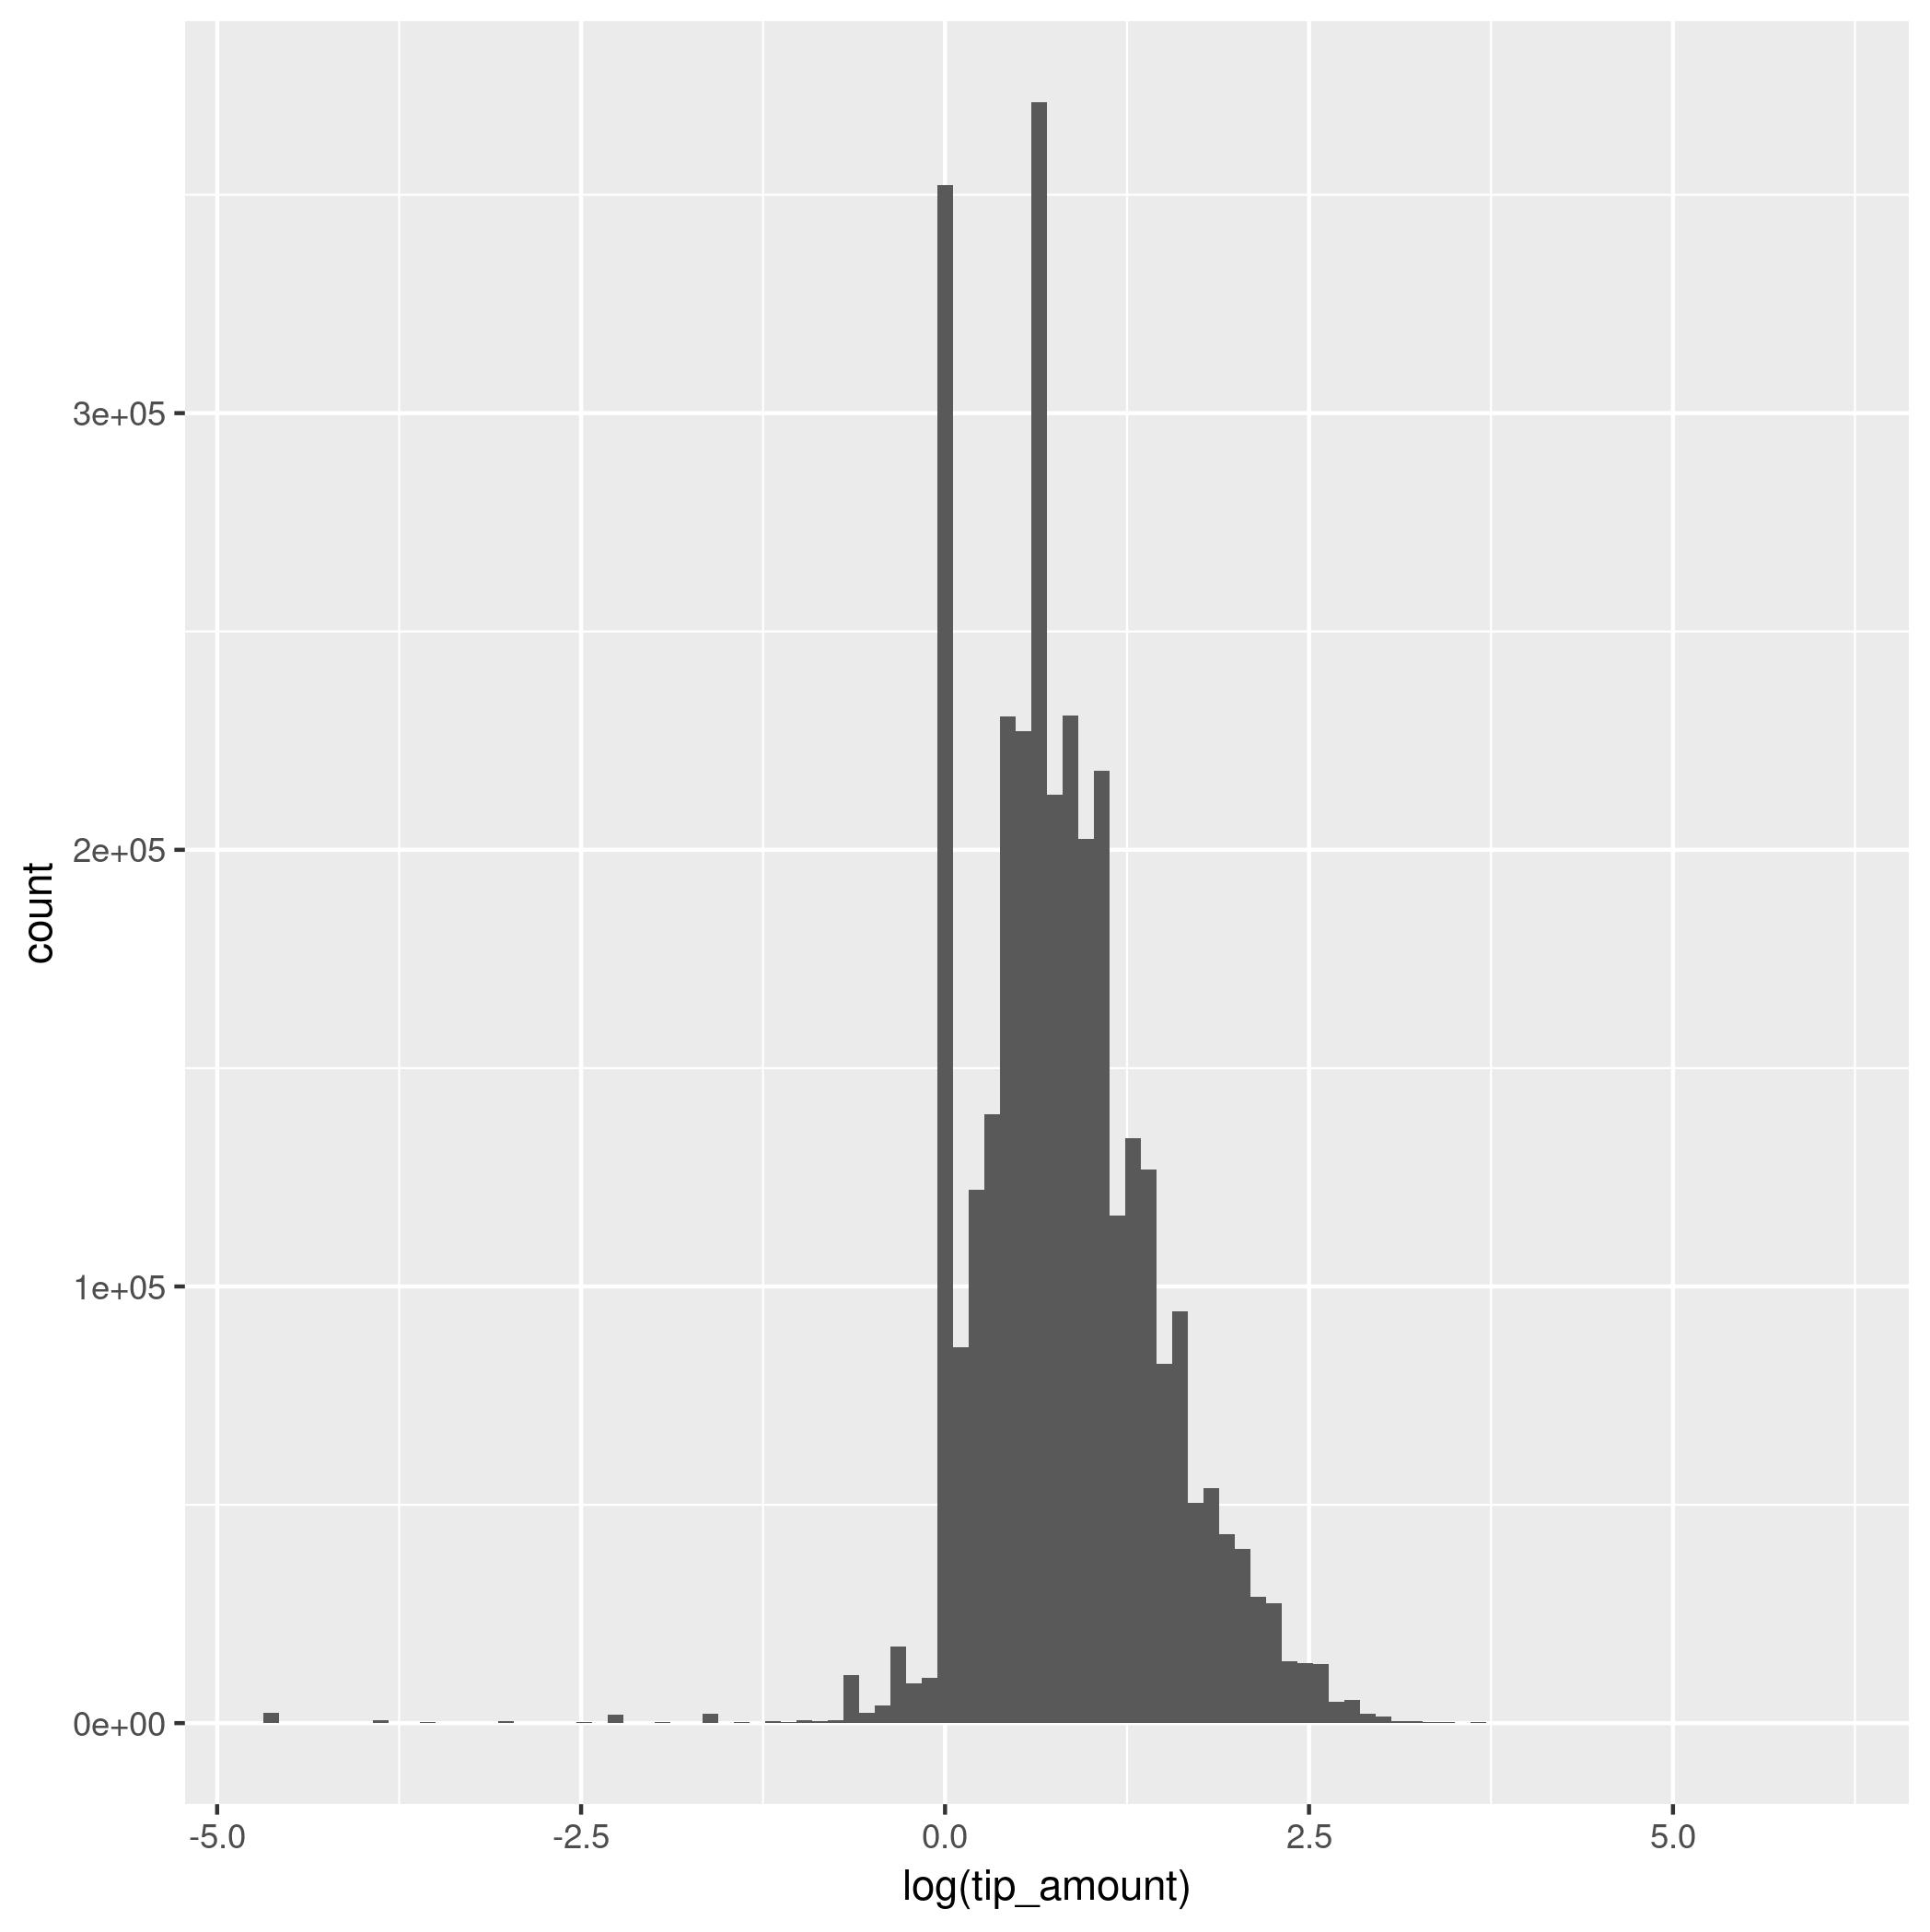
\includegraphics[width=.9\linewidth]{./plots/logTipHist.jpg}
\caption{\label{fig:orga1fd2ea}
Log-tip histogram}
\end{figure}

Approximation of a normal might be over stated, but it does not look to bad.
strong peaks at 0 (tip of \$1) and below 1.5, roughly arround the mean,
(tip of about \$2) make perfect sense. There is a long tail on the negative
side, these are people that are tipping too little. Probably they need to
be treated too.

Next, we look at the same distribution, but color coding if the tip was
larger than the actual fare in red (generous tip), and blue otherwise
(standard tip).

\begin{figure}[htbp]
\centering
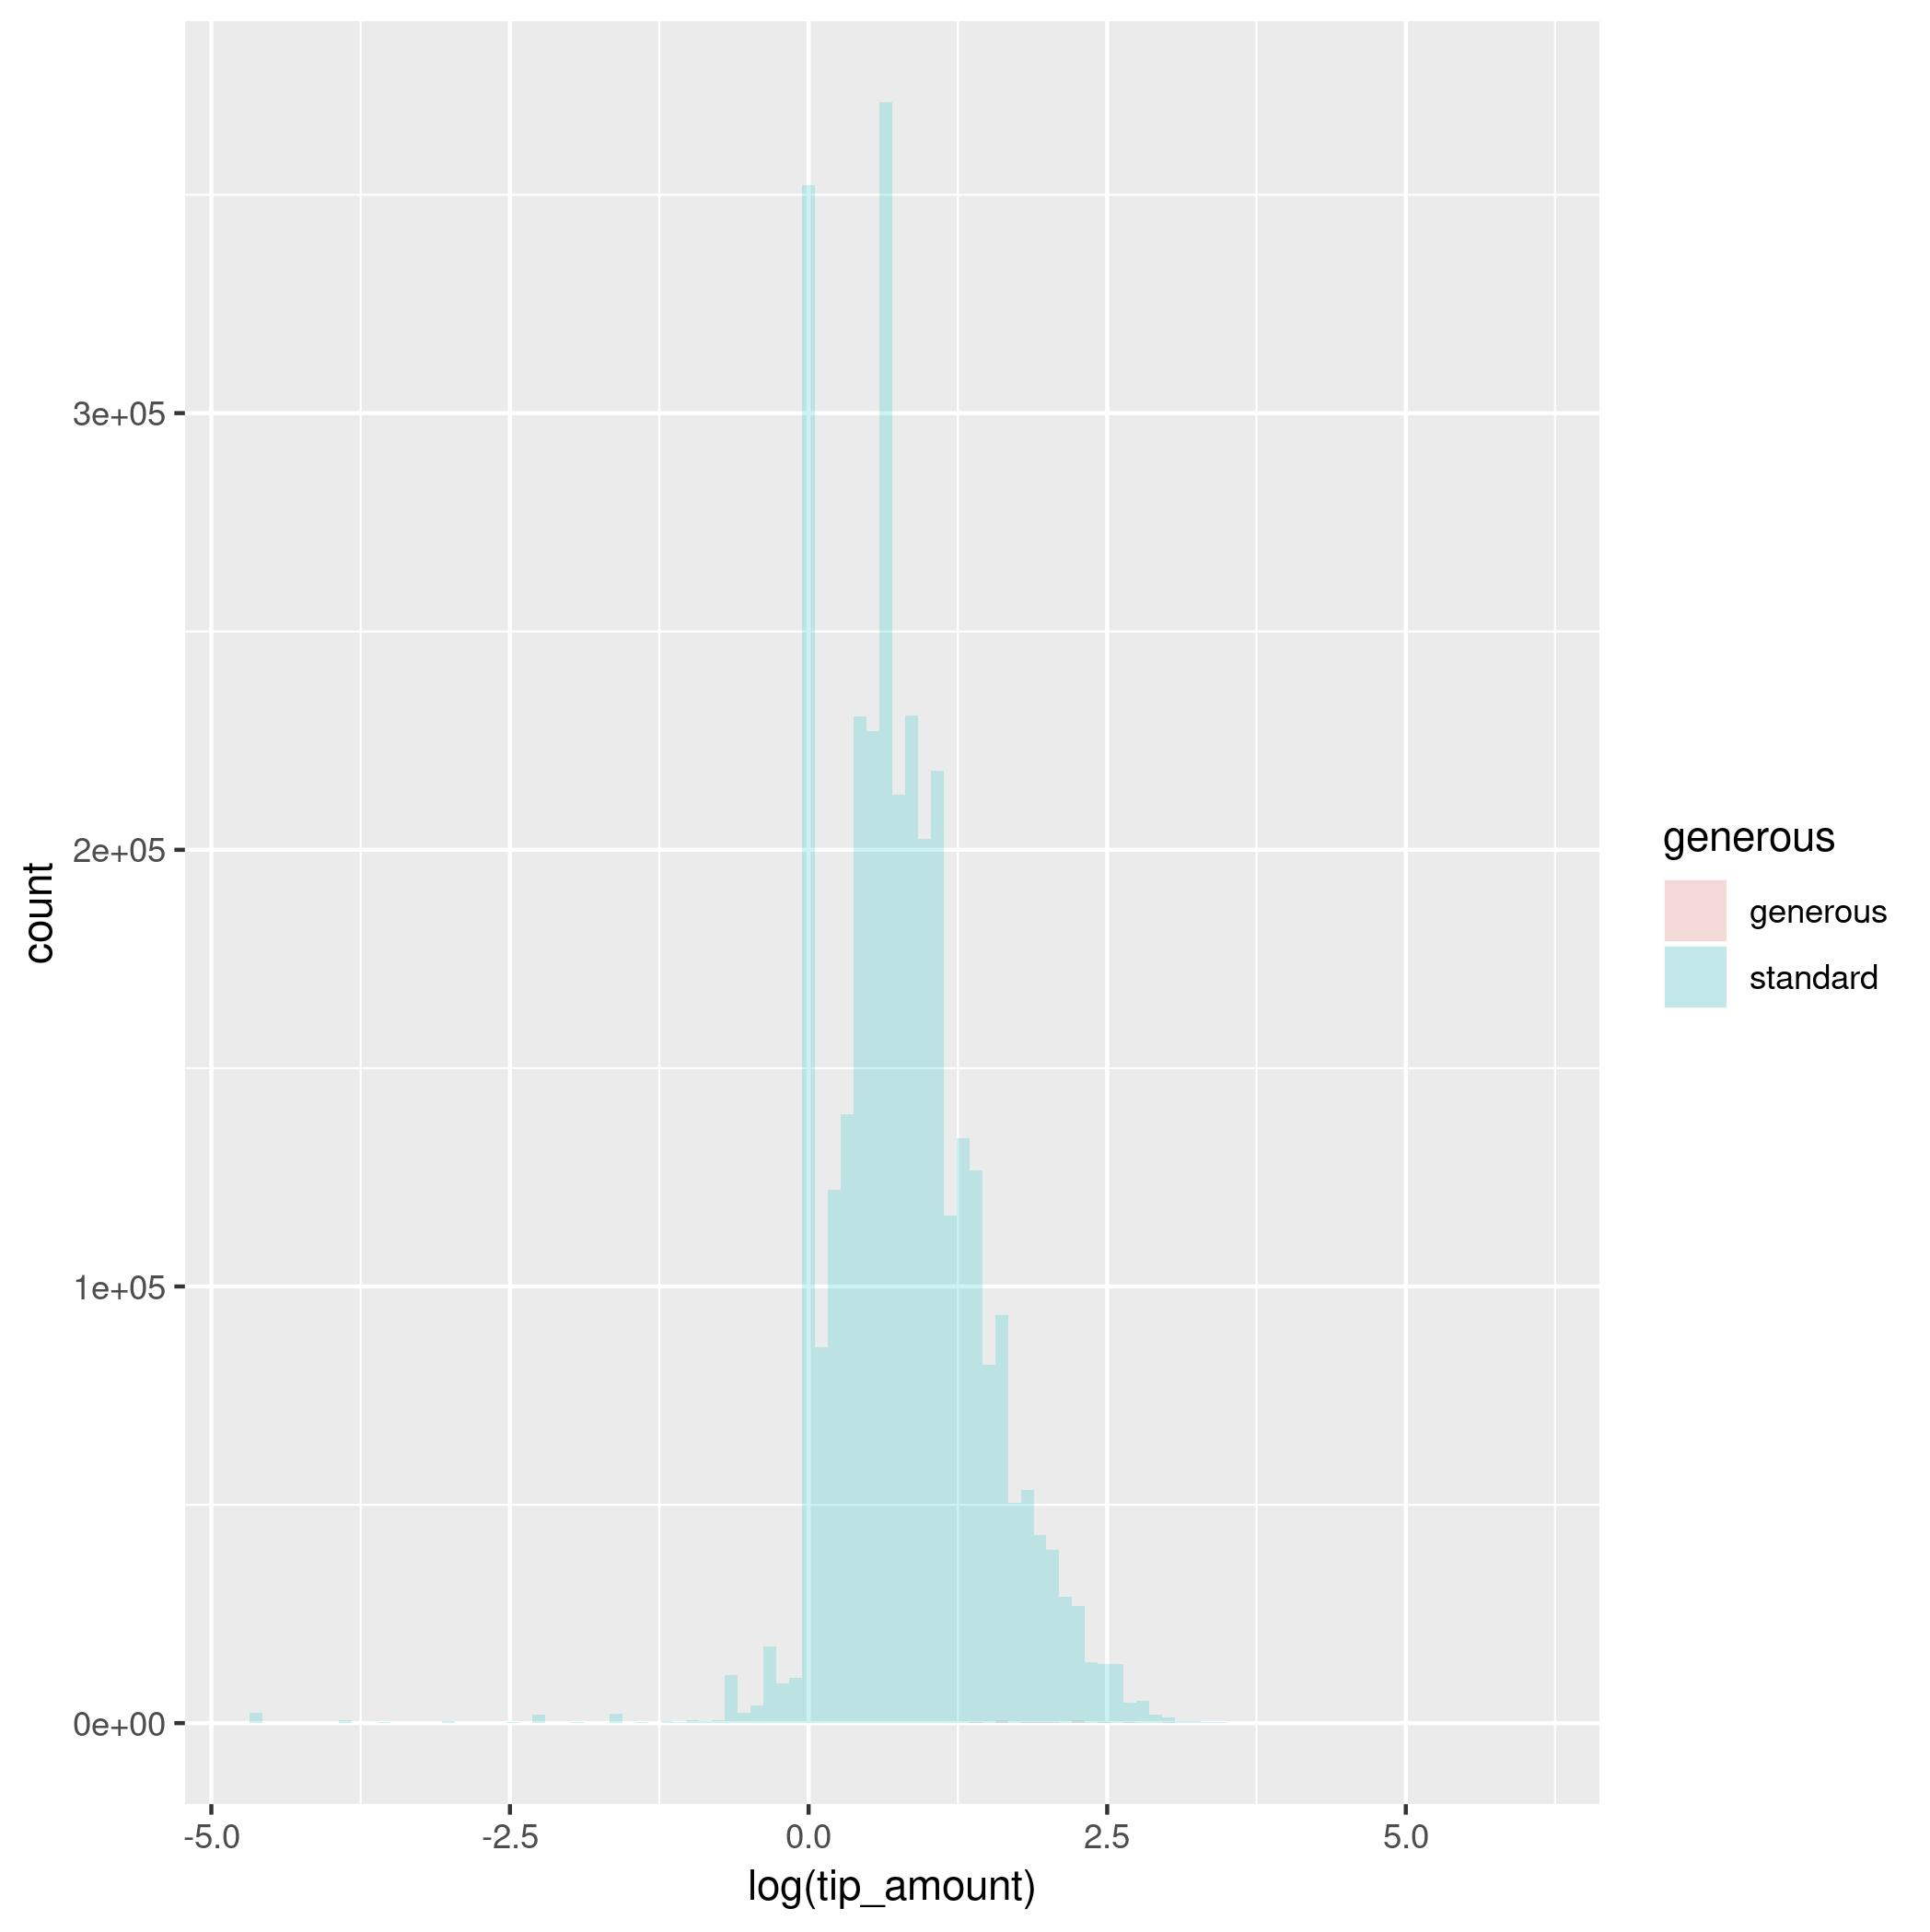
\includegraphics[width=.9\linewidth]{./plots/logTipGenerousHist.jpg}
\caption{\label{fig:org4b7957e}
Log-tip histogram by class of tip}
\end{figure}

We see no noticiable behaviour on this scale, which means that generous tips are
rather rare. So we probably need to look at the densities rahter than counts.

\begin{figure}[htbp]
\centering
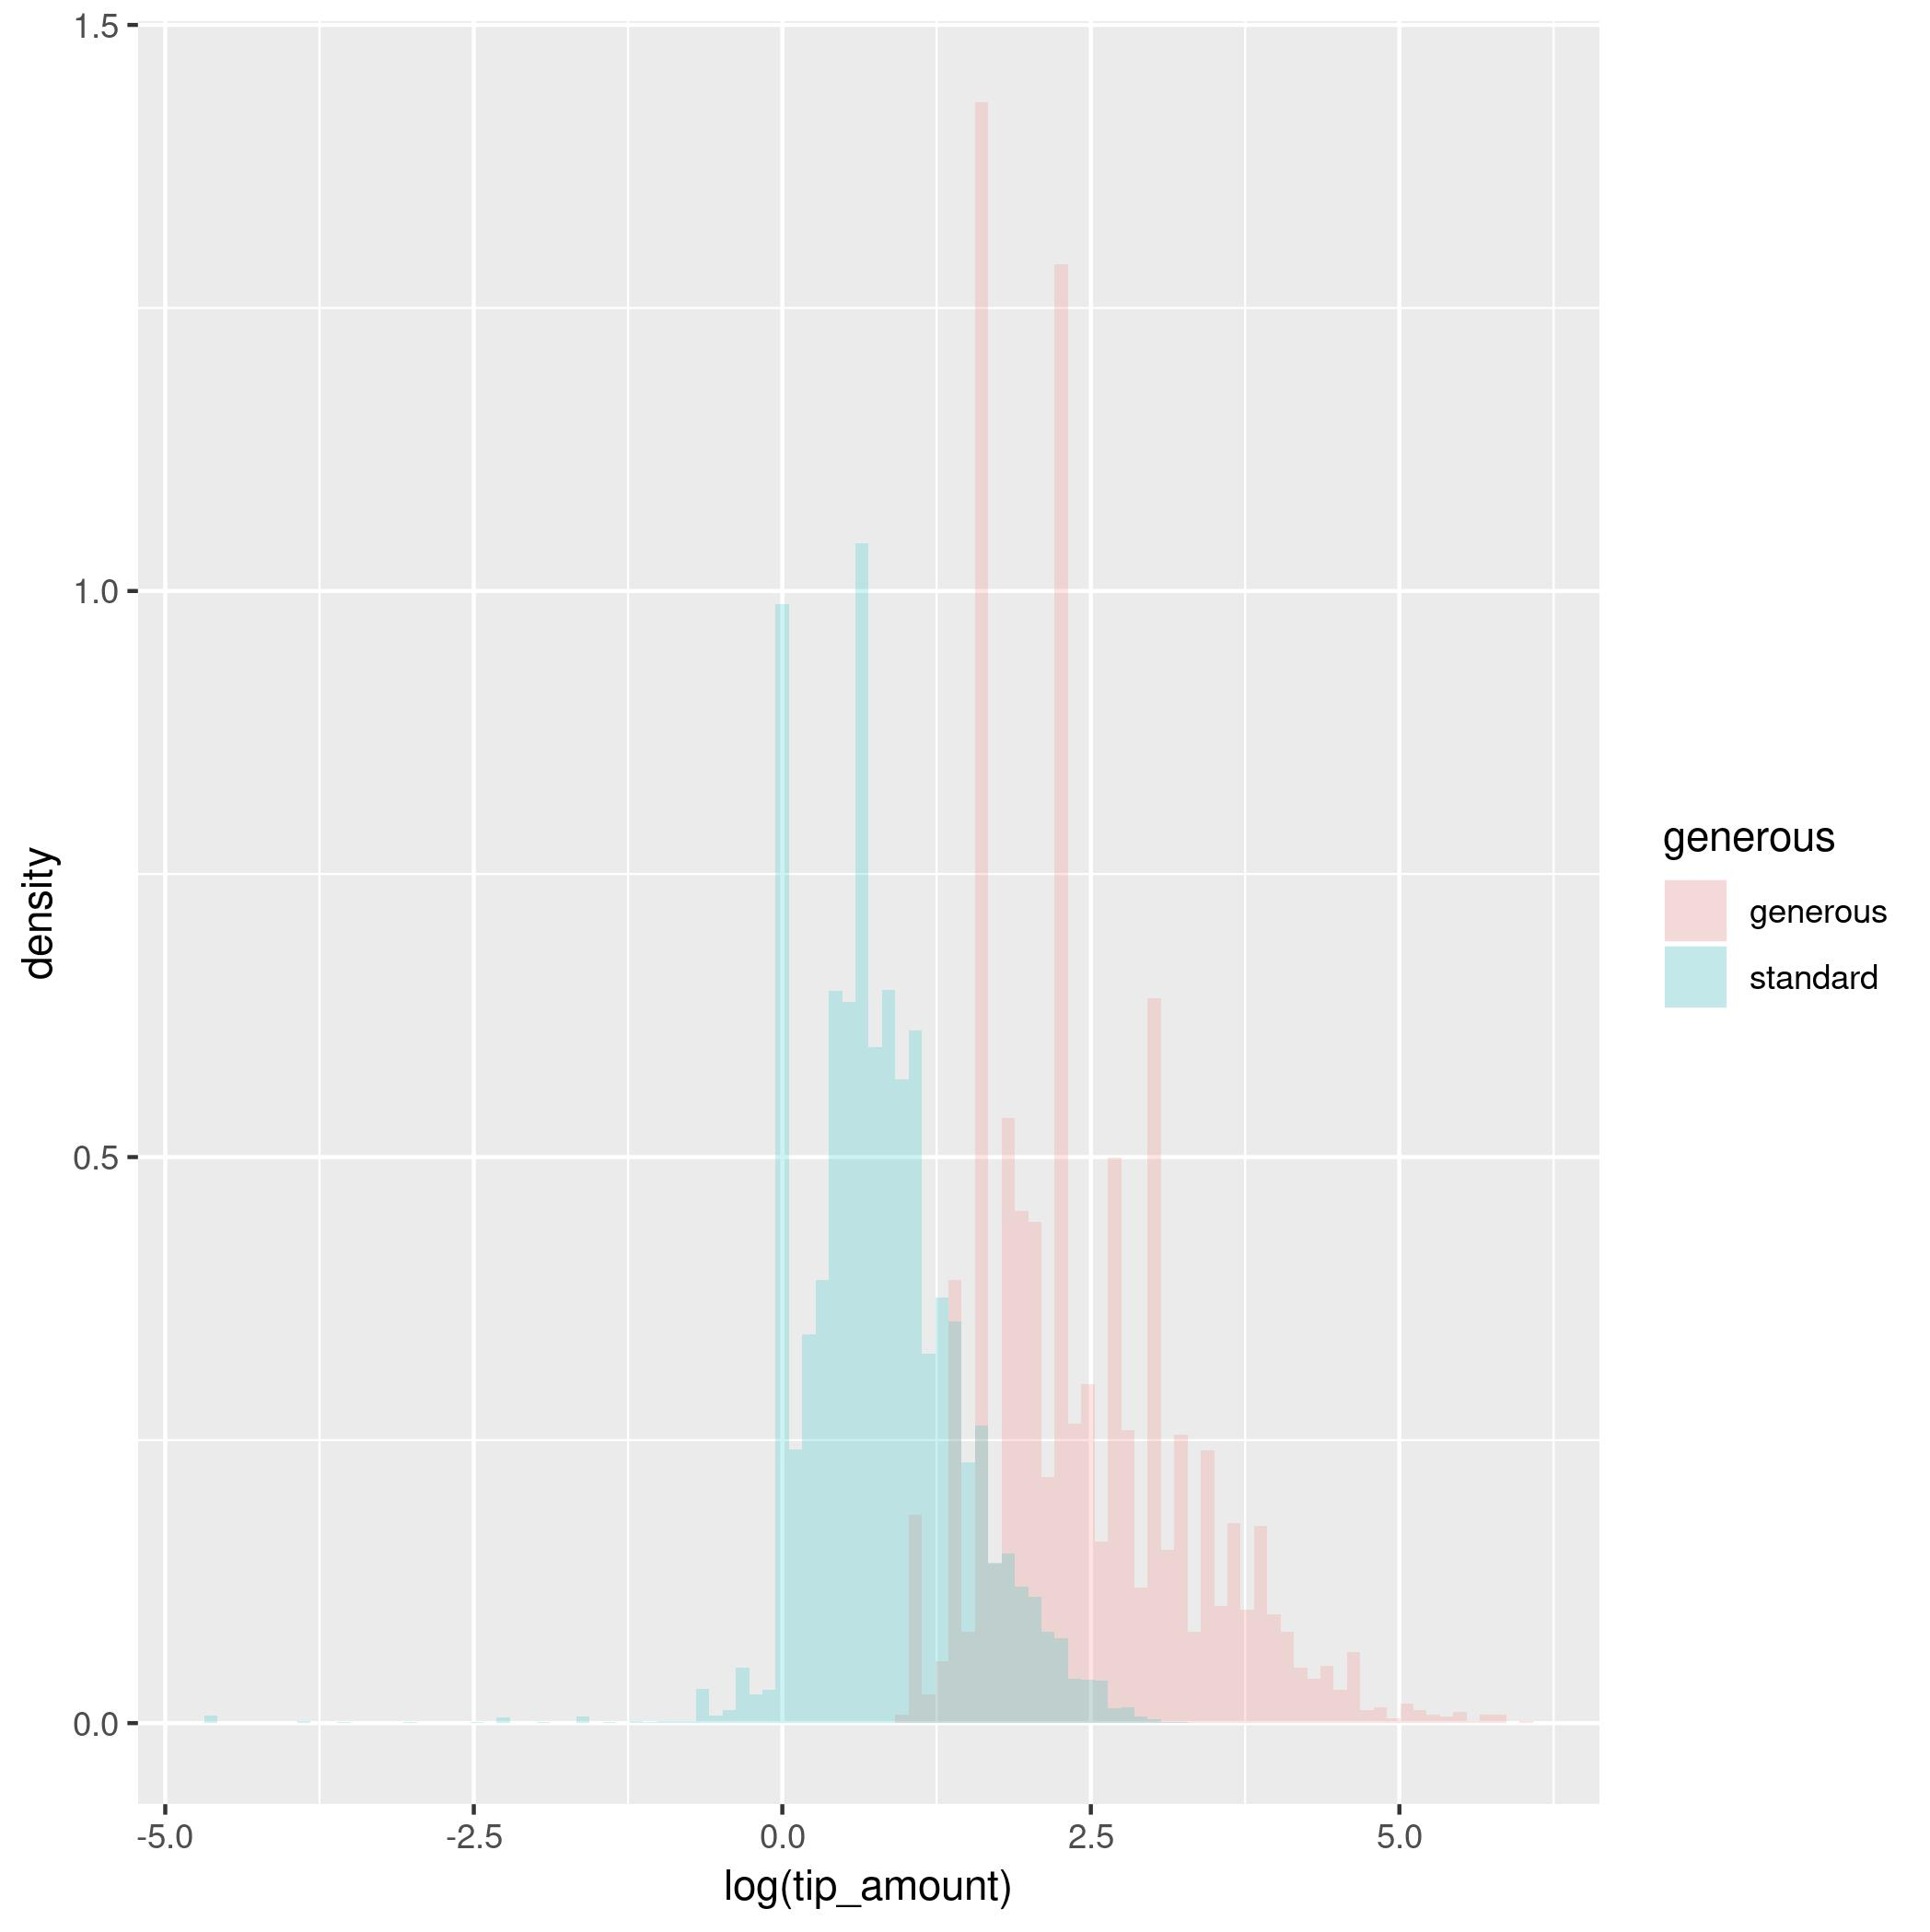
\includegraphics[width=.9\linewidth]{./plots/logTipGenerousFrequencyHist.jpg}
\caption{\label{fig:org91a8b09}
Log-tip density histogram by class of tip}
\end{figure}

This looks interesting, the blue distribution looks similar to the first plot,
but generous tips have a higher mean and standard distribution than standard
tips.

In order to have a better understanding of the data, and figure out what to do
with these obvservations, we will compare them with the fee amount.

\begin{verbatim}
library("tidyverse")
library("ggplot2")
library("lubridate")

data <- readRDS("taxiDataFeatures.rds") %>%
    select(tip_amount, fare_amount, relativeTip)

data <- data %>% mutate(generous = relativeTip %>%
                            sapply(function(x) {
                                if (x > 1) "generous"
                                else "standard"
                            }))

plotsFolder <- "plots"
fareTipPlot <- ggplot(data = data, aes(x = fare_amount, y = tip_amount,
                                       color = generous)) +
    geom_point()

ggsave(paste(plotsFolder, "fareTipPlot.jpg", sep = "/"),  fareTipPlot)


logFareTipPlot <- ggplot(data = data, aes(x = log(fare_amount), y = log(tip_amount),
                                       color = generous)) +
    geom_point()

ggsave(paste(plotsFolder, "logFareTipPlot.jpg", sep = "/"),  logFareTipPlot)

fareTipStandardPlot <- ggplot(data = data %>% filter(generous == "standard"),
                      aes(x = log(fare_amount), y = log(tip_amount))) +
    geom_point()

ggsave(paste(plotsFolder, "logFareTipStandardPlot.jpg", sep = "/"),  fareTipStandardPlot)

fareTip100Plot <- ggplot(data = data %>% filter(tip_amount < 100),
                      aes(x = log(fare_amount), y = log(tip_amount))) +
    geom_point()

ggsave(paste(plotsFolder, "logFareTip100Plot.jpg", sep = "/"),  fareTip100Plot)
\end{verbatim}
\begin{figure}[htbp]
\centering
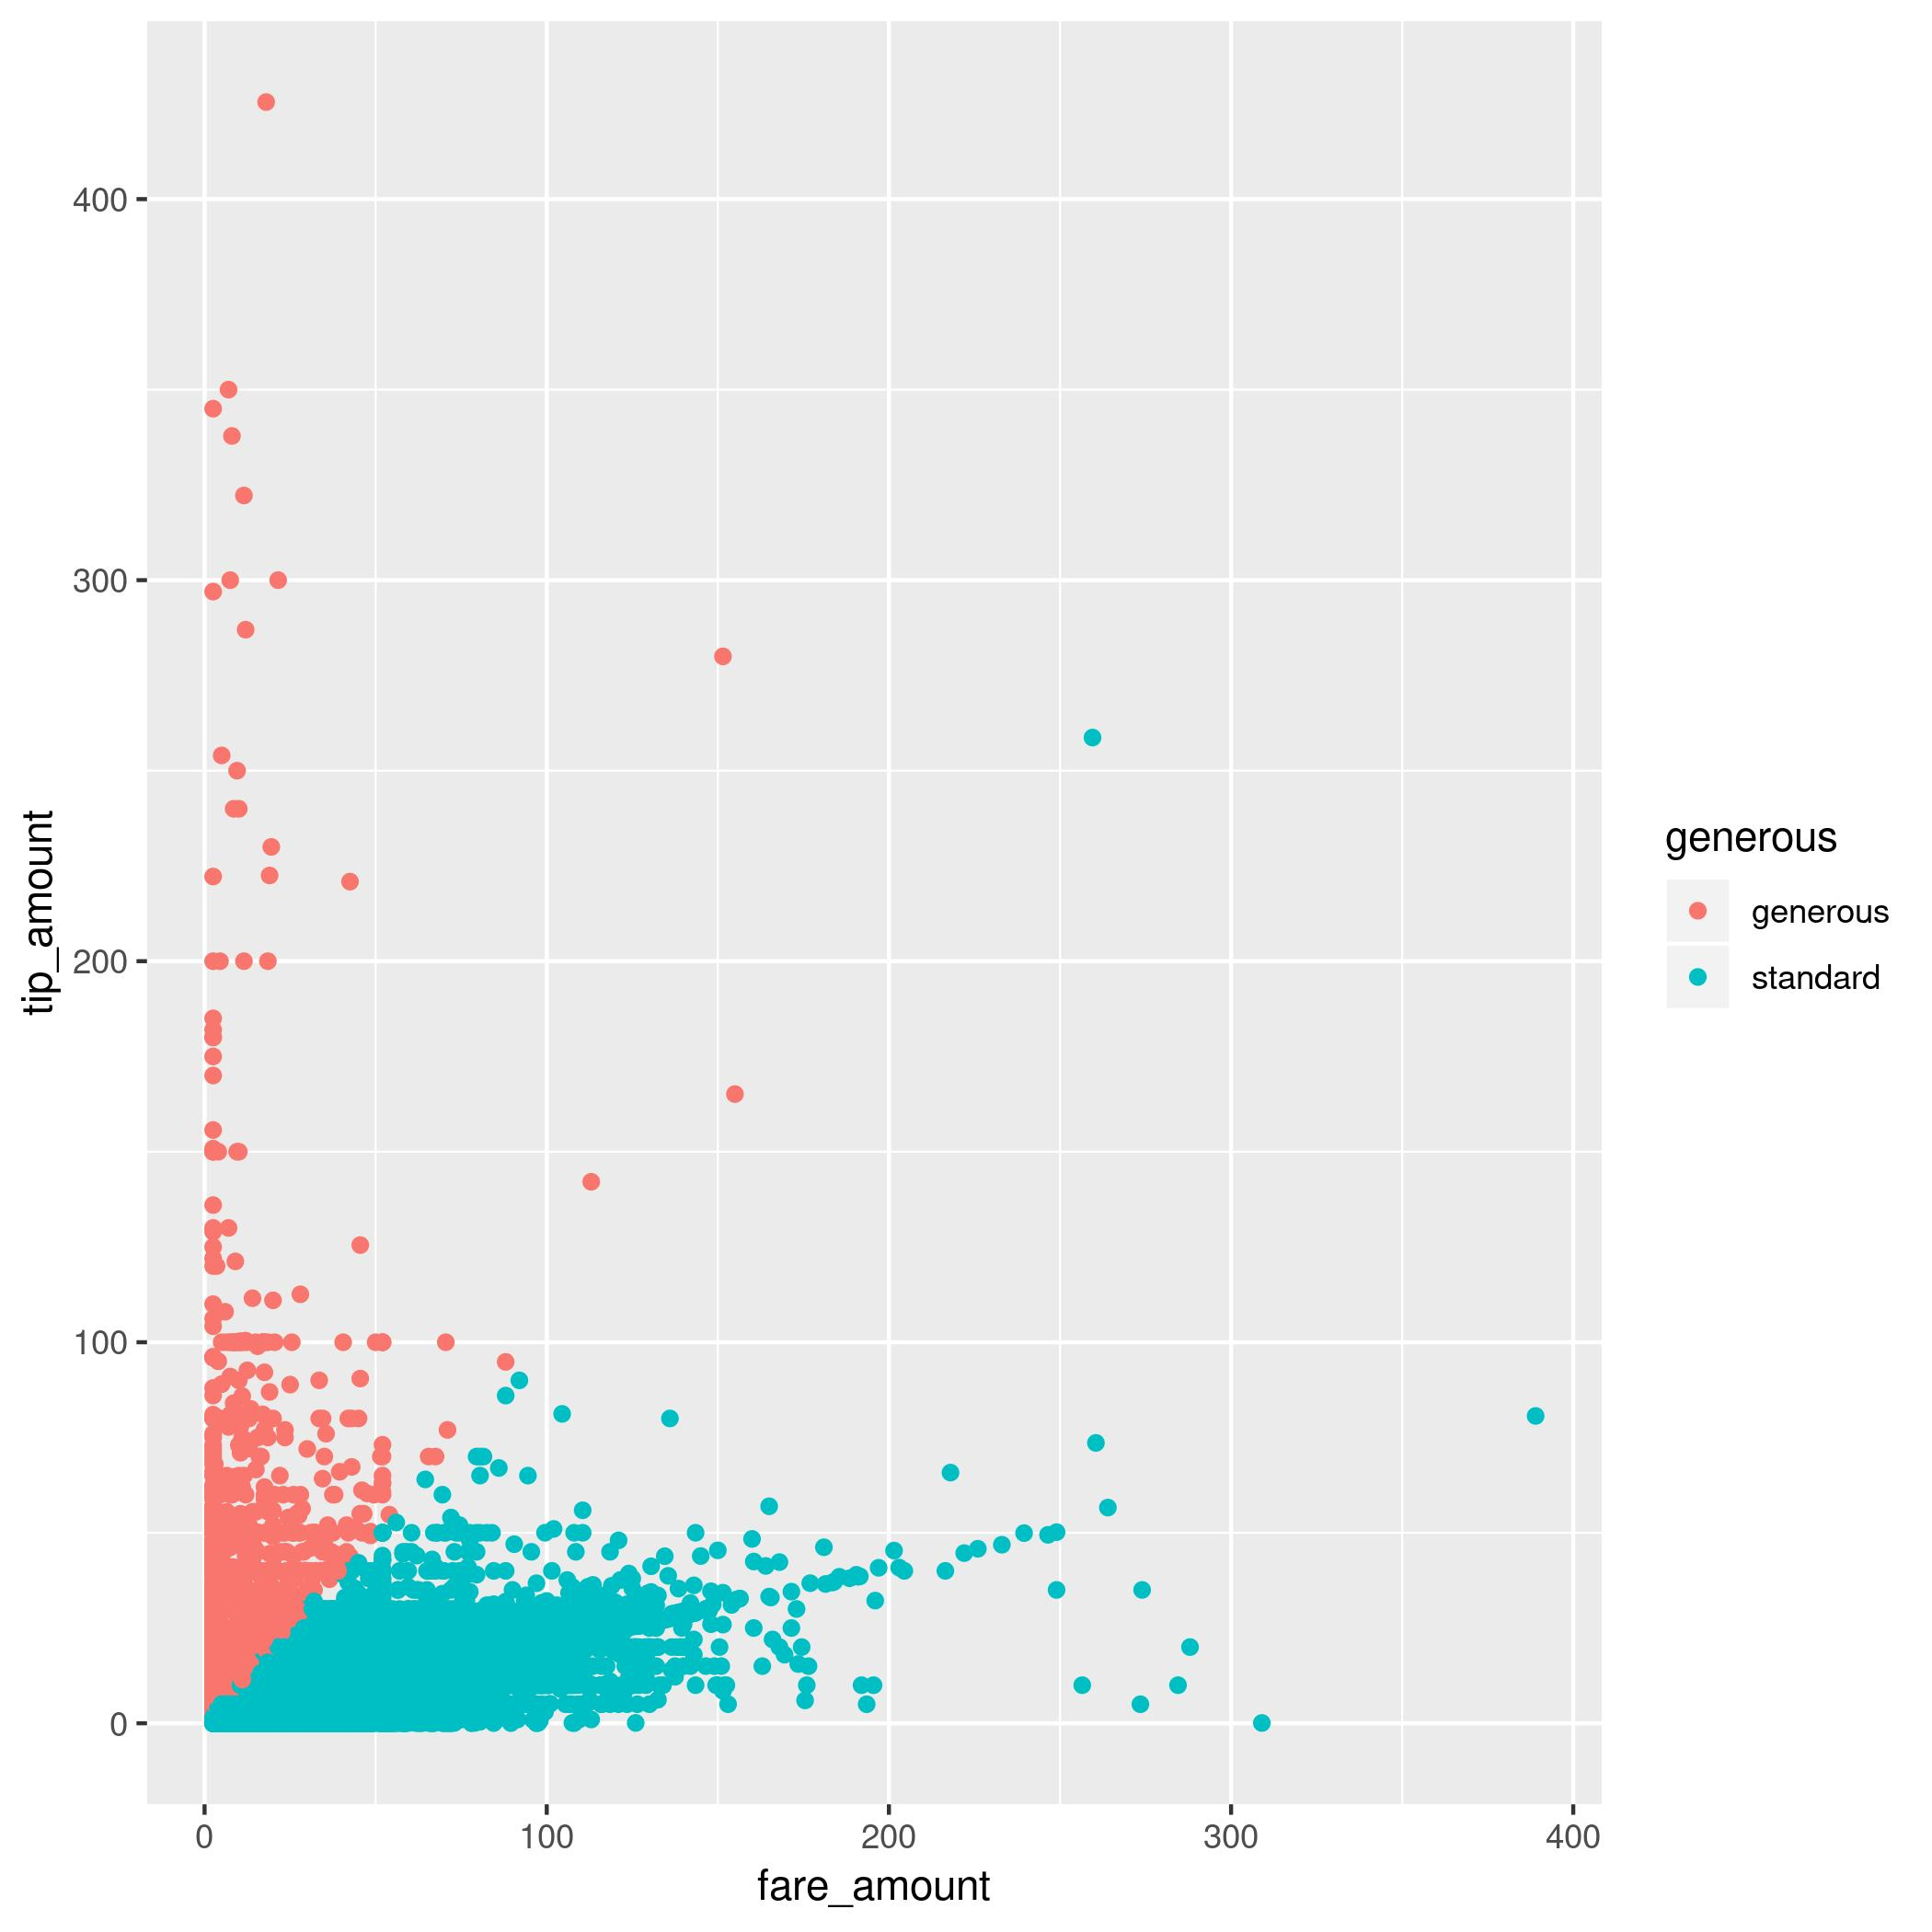
\includegraphics[width=.9\linewidth]{./plots/fareTipPlot.jpg}
\caption{\label{fig:org3d65f2e}
fare vs tip scatterplot}
\end{figure}

In this plot we can notice that tips of over \$100 tend to be clustered
under \$50 fares. Filtering out tips over \$100 might be a good compromise
solution to clean the \emph{tip\_amount} variable. Filtering tips of over \$200
might be a better choice, but once again, i am taking into consideration
hardware restrictions.

\begin{figure}[htbp]
\centering
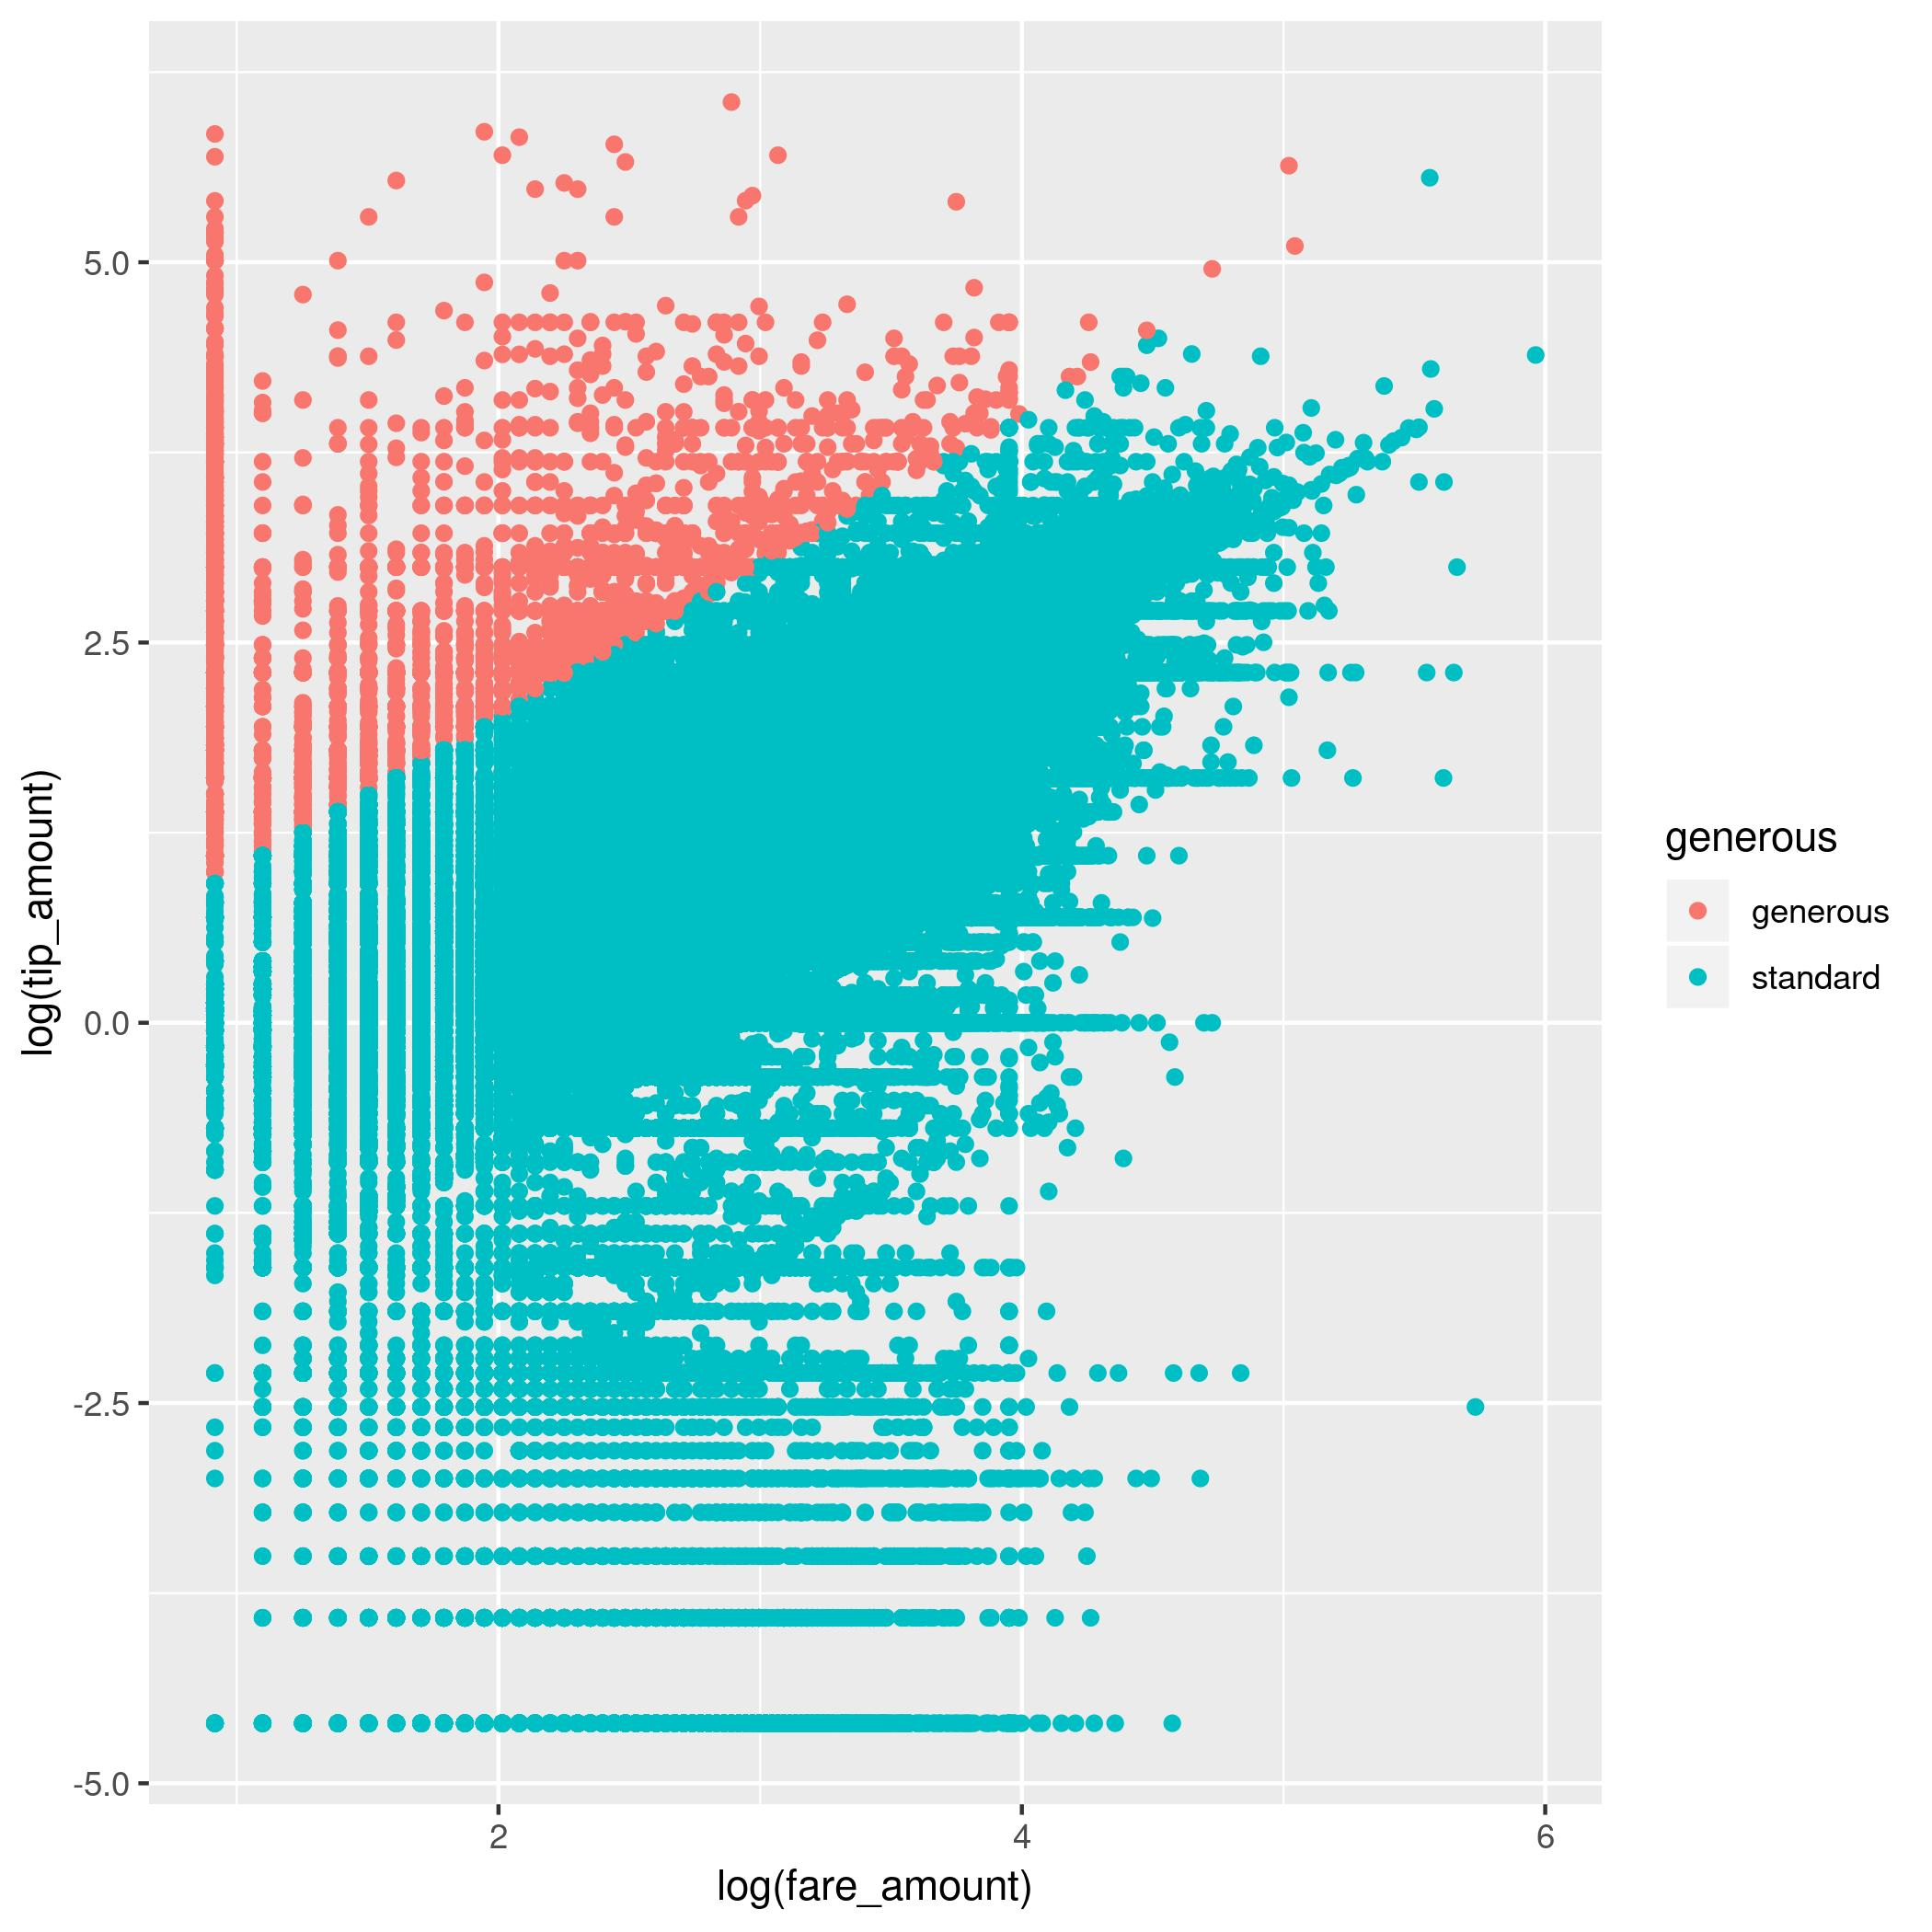
\includegraphics[width=.9\linewidth]{./plots/logFareTipPlot.jpg}
\caption{\label{fig:orgd288986}
log-fare vs log-tip scatterplot}
\end{figure}

In the log scale, there is a clearer positive correlation betweem the two
variables.

The next two plots display the scatterplot of log tip vs log fares under two
filter approaches: 1) removing all tips greater than the fares, 2) removing
tips over \$100. The latter approach seems more sensible, as it mantains better
the original distribution of the data. but maybe this is a none issue. 

\begin{figure}[htbp]
\centering
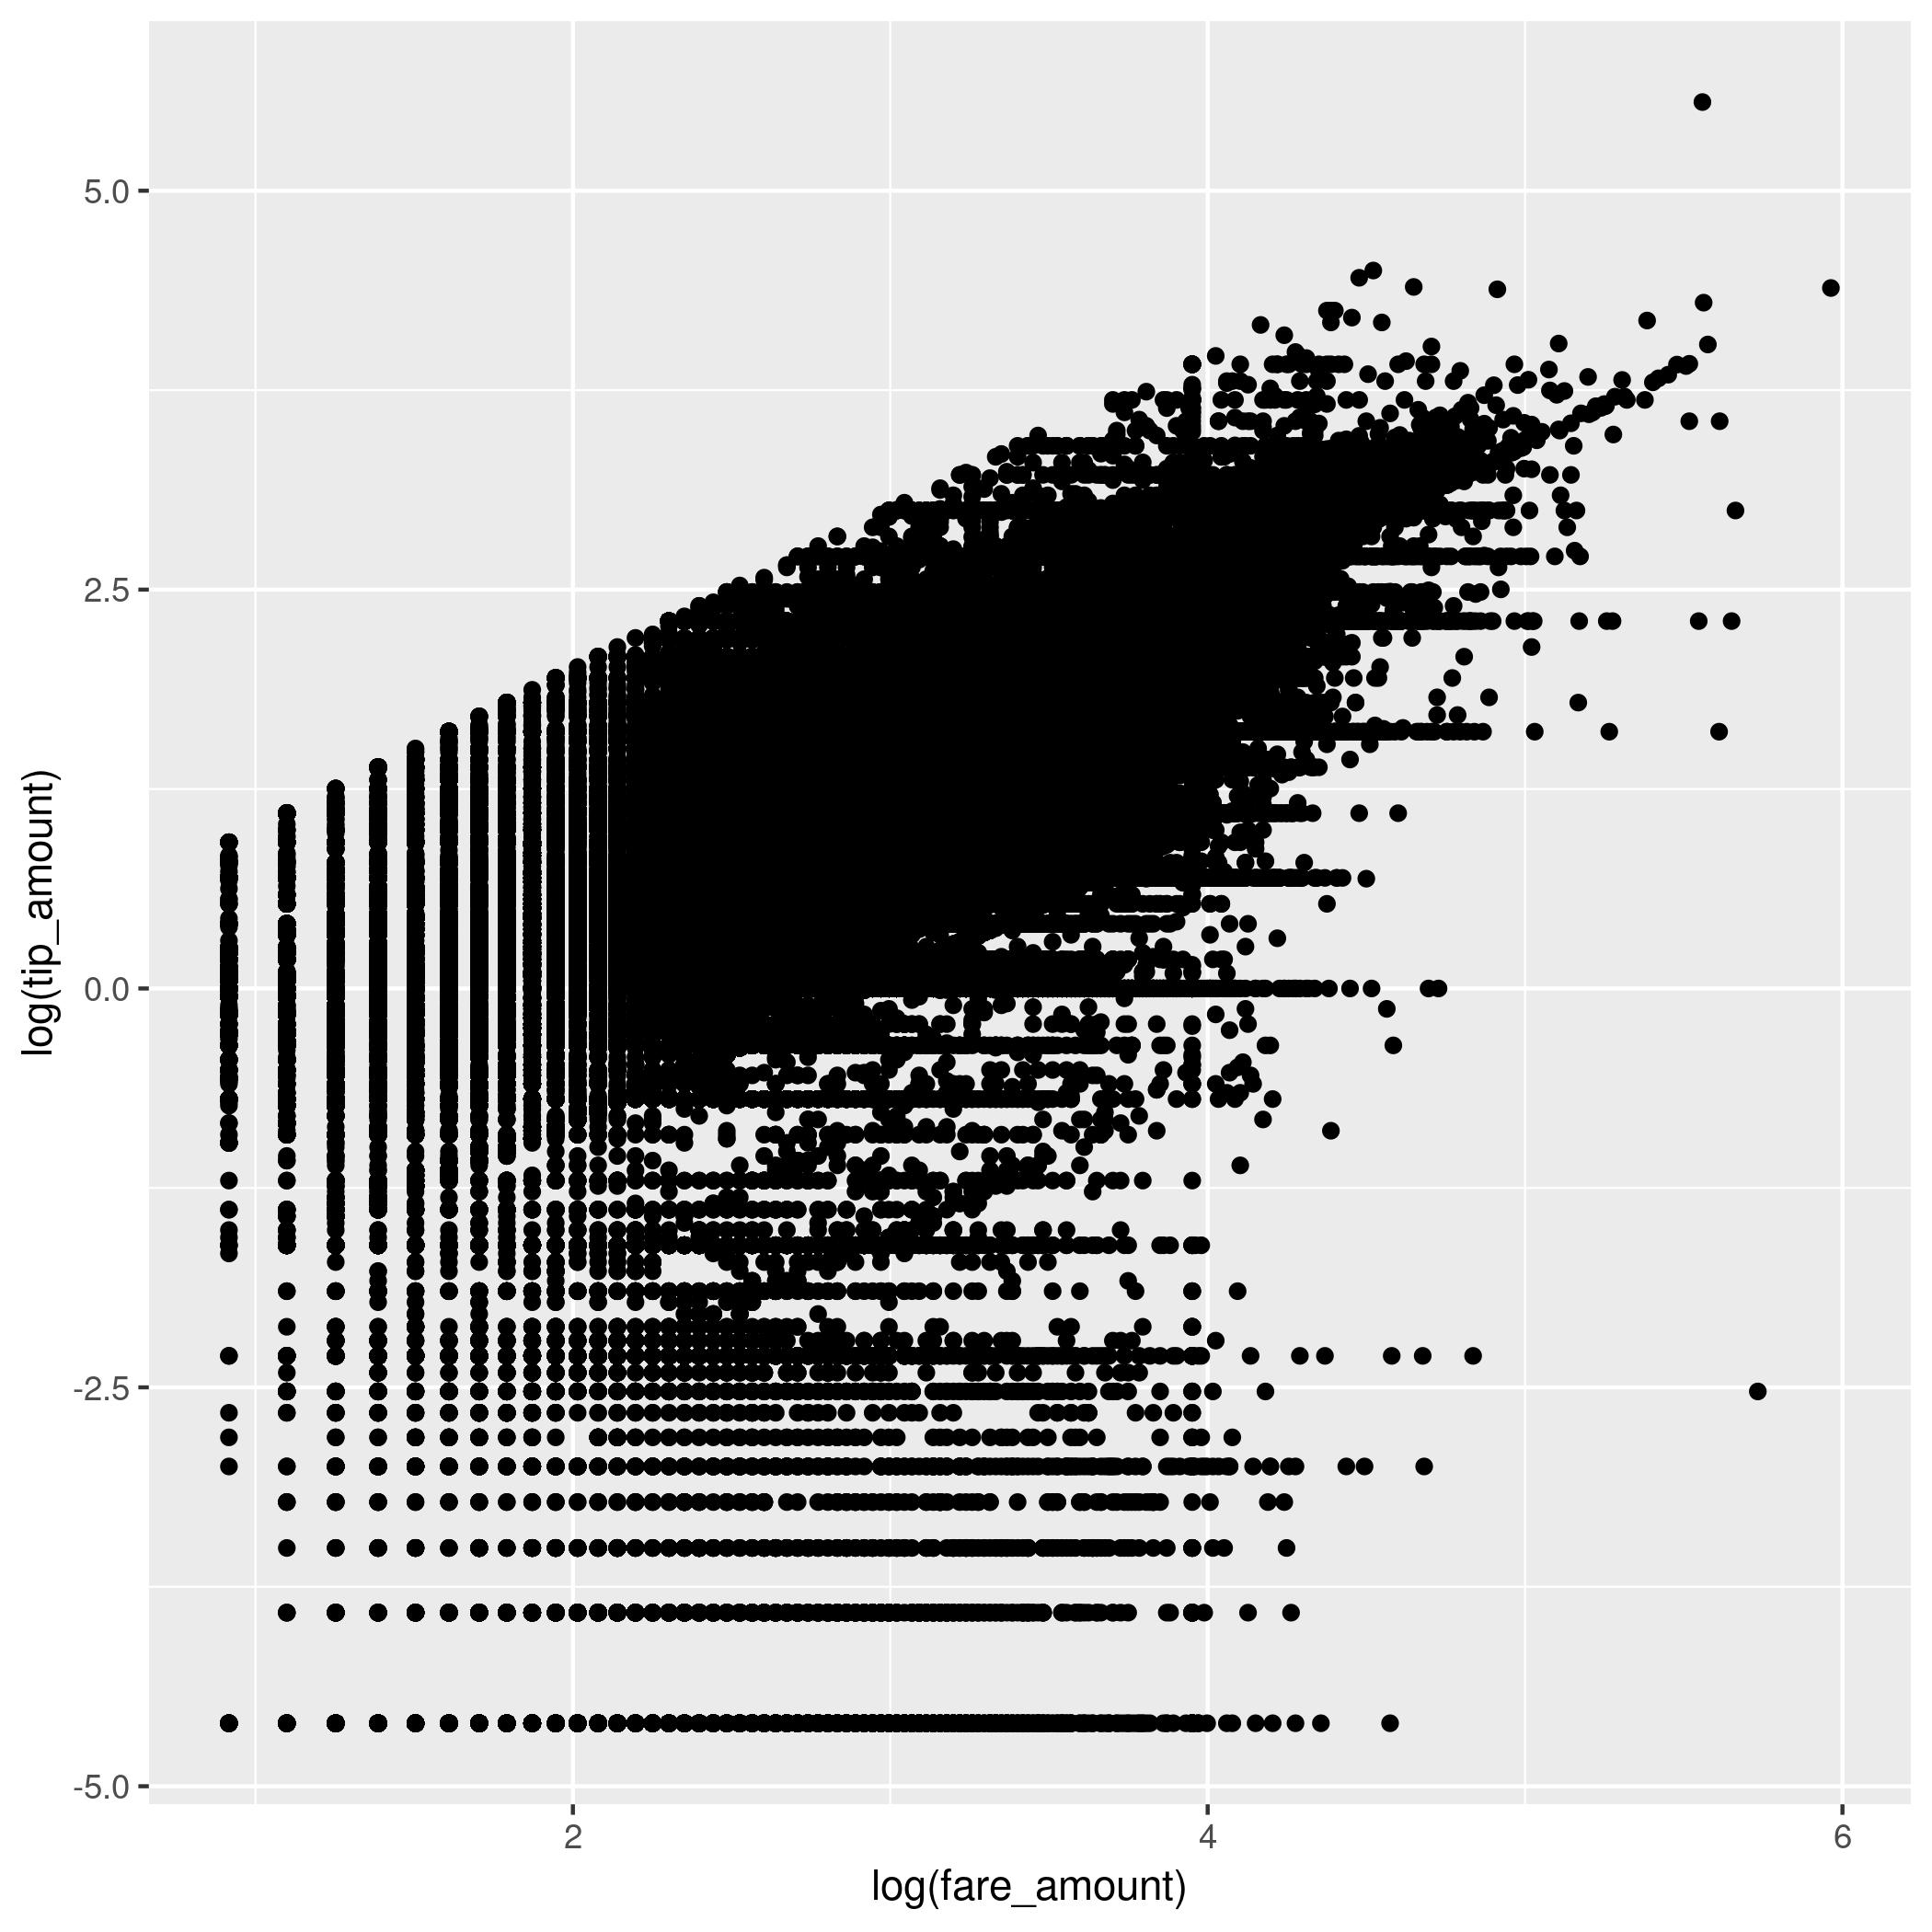
\includegraphics[width=.9\linewidth]{./plots/logFareTipStandardPlot.jpg}
\caption{\label{fig:org8b1c348}
Log-tip density histogram by class of tip}
\end{figure}

\begin{figure}[htbp]
\centering
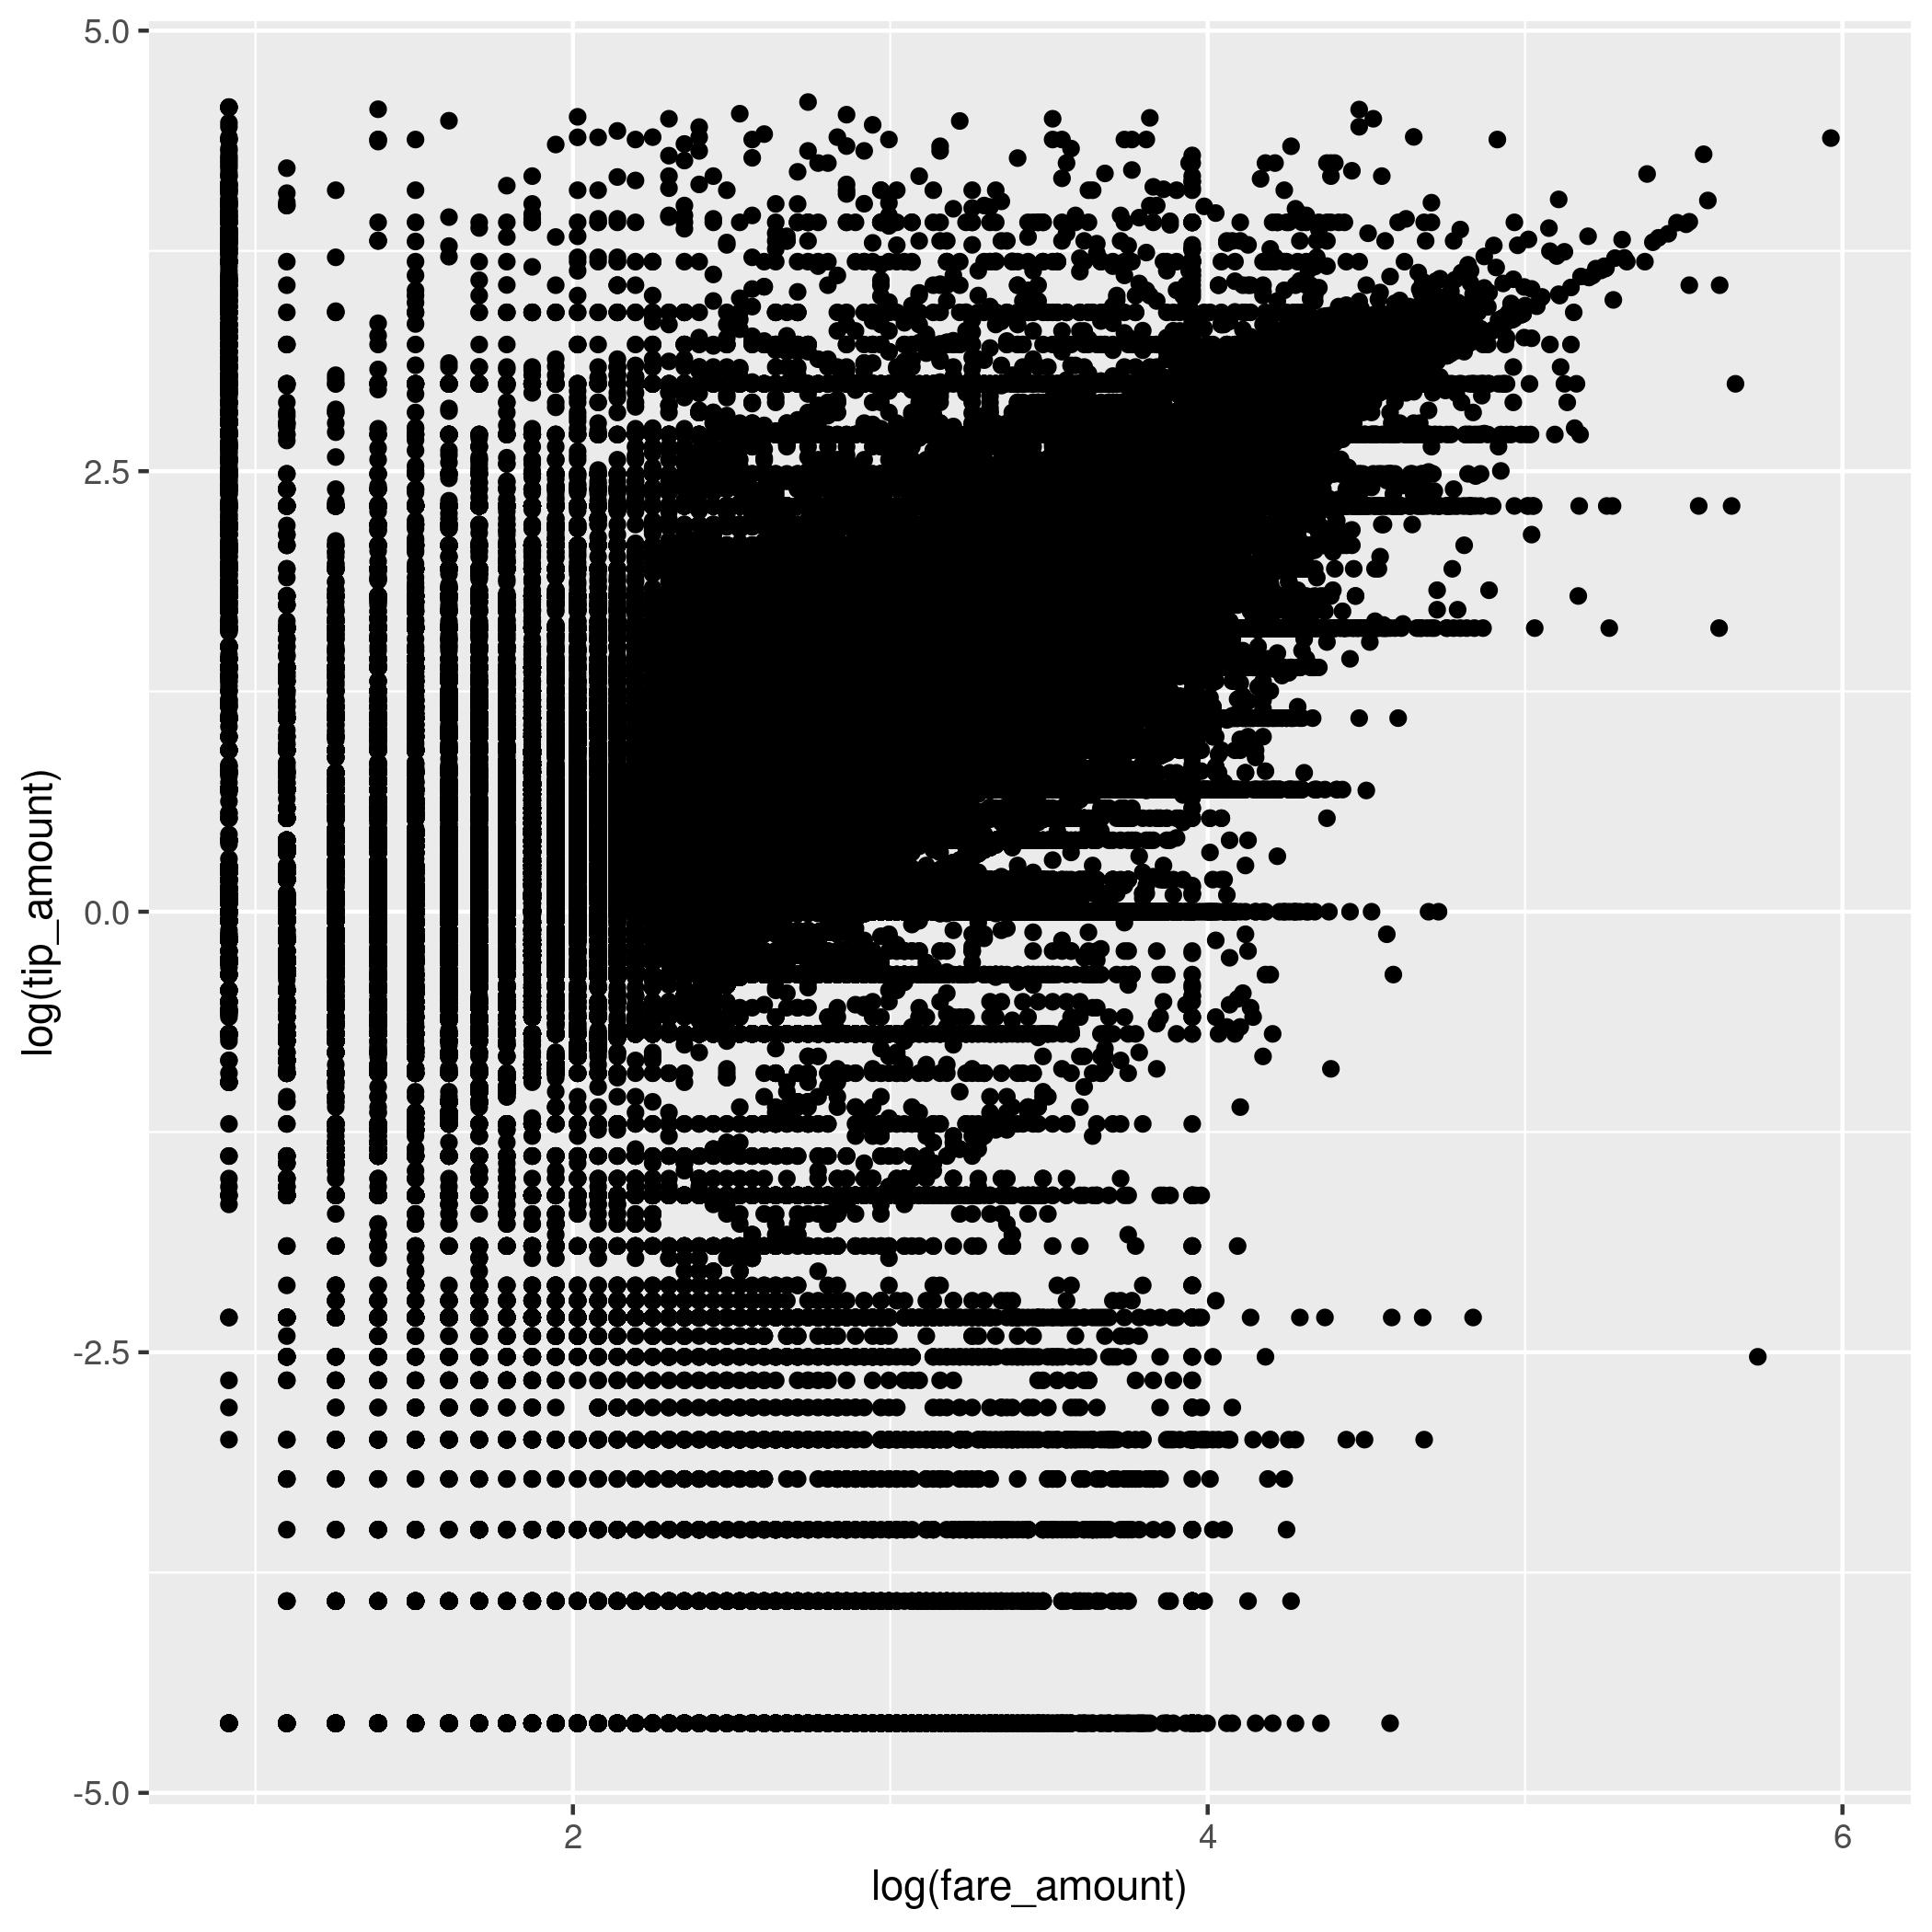
\includegraphics[width=.9\linewidth]{./plots/logFareTip100Plot.jpg}
\caption{\label{fig:org161d101}
Log-tip density histogram by class of tip}
\end{figure}


\subsection{visualizations}
\label{sec:org9944dbd}
\begin{verbatim}
library("tidyverse")
library("ggplot2")

workDays <- c("jueves", "miércoles", "viernes", "lunes", "martes")
weekEnd <- c("domingo", "sábado")
plotsFolder <- "plots"
data <- readRDS("taxiDataFeatures.rds") %>%
    filter(tip_amount < 100) %>% 
    mutate(generous = relativeTip %>%
               sapply(function(x) {
                   if (x > 1) "generous"
                   else "standard"
               })) %>%
    mutate(weekEnd = weekDay %>%
           sapply(function(x)
                  if (x %in% workDays) "workDay"
                  else if (x %in% weekEnd) "weekEnd"
                  else "badDay")) %>%
    mutate(tollPaid = tolls_amount %>%
               sapply(function(x)
                      if (x == 0) "noToll"
                      else if(x > 0) "tollPaid"
                      else "badToll"))
## data %>% saveRDS("taxiDataFinal.rds")
data %>% colnames
passengerTipBox <- ggplot(data = data,
       aes(x = as.factor(passenger_count), y = log(tip_amount),
           group = passenger_count)) +
    geom_boxplot()
ggsave(paste(plotsFolder, "passengerTipBox.jpg", sep = "/"),  passengerTipBox)

## weekendTipHist <- ggplot(data = data, aes(log(tip_amount), fill = weekEnd)) +
##     geom_histogram(bins = 100, position = "identity", alpha = 0.2)
## ggsave(paste(plotsFolder, "weekendTipHist.jpg", sep = "/"),  weekendTipHist)

weekendTipDensityHist <- ggplot(data = data, aes(x = log(tip_amount),
                                                 y = stat(density), fill = weekEnd)) +
    geom_histogram(bins = 100, position = "identity", alpha = 0.2)
ggsave(paste(plotsFolder, "weekendTipDensityHist.jpg", sep = "/"),  weekendTipDensityHist)

## dayPeriodTipHist <- ggplot(data = data, aes(log(tip_amount), fill = dayPeriod)) +
##     geom_histogram(bins = 100, position = "identity", alpha = 0.2)
## dayPeriodTipHist
## ggsave(paste(plotsFolder, "dayPeriodTipHist.jpg", sep = "/"),  weekendTipHistp)

dayPeriodTipDensityHist <- ggplot(data = data, aes(x = log(tip_amount),
                                                   y = stat(density), fill = dayPeriod)) +
    geom_histogram(bins = 100, position = "identity", alpha = 0.2)
ggsave(paste(plotsFolder, "dayPeriodTipDensityHist.jpg", sep = "/"),  dayPeriodTipDensityHist)

paymentTipDensityHist <- ggplot(data = data, aes(x = log(tip_amount),
                        y = stat(density), fill = as.factor(payment_type))) +
    geom_histogram(bins = 100, position = "identity", alpha = 0.2)
ggsave(paste(plotsFolder, "paymentTipDensityHist.jpg", sep = "/"),  paymentTipDensityHist)

storeCodeTipDensityHist <- ggplot(data = data, aes(x = log(tip_amount),
                        y = stat(density), fill = as.factor(store_and_fwd_flag))) +
    geom_histogram(bins = 100, position = "identity", alpha = 0.2)
ggsave(paste(plotsFolder, "storeCodeTipDensityHist.jpg", sep = "/"), storeCodeTipDensityHist)

rateCodeTipDensityHist <- ggplot(data = data, aes(x = log(tip_amount),
                        y = stat(density), fill = as.factor(RatecodeID))) +
    geom_histogram(bins = 100, position = "identity", alpha = 0.2)
ggsave(paste(plotsFolder, "rateCodeTipDensityHist.jpg", sep = "/"), rateCodeTipDensityHist)

logTripDistanceHist <- ggplot(data = data, aes(log(trip_distance))) +
    geom_histogram(bins = 100)
ggsave(paste(plotsFolder, "logTripDistanceHist.jpg", sep = "/"), logTripDistanceHist)

distanceTipPlot <- ggplot(data = data,
                          aes(x = log(trip_distance), y = log(tip_amount))) +
    geom_point()
ggsave(paste(plotsFolder, "distanceTipPlot.jpg", sep = "/"), distanceTipPlot)

tollsTipPlot <- ggplot(data = data,
                       aes(x = tolls_amount, y = log(tip_amount))) + geom_point()
ggsave(paste(plotsFolder, "tollsTipPlot.jpg", sep = "/"), tollsTipPlot)

tollsTipDensityHist <- ggplot(data = data,
                              aes(x = log(tip_amount), y = stat(density),
                                  fill = as.factor(tollPaid))) +
    geom_histogram(bins = 100, position = "identity", alpha = 0.2)
ggsave(paste(plotsFolder, "tollsTipDensityHist.jpg", sep = "/"), tollsTipDensityHist)

rideTimeHist <- ggplot(data = data, aes(log(rideTime))) + geom_histogram(bins = 100)
ggsave(paste(plotsFolder, "rideTimeHist.jpg", sep = "/"), rideTimeHist)
rideTipPlot <- ggplot(data = data, aes(x = log(rideTime),
                                       y = log(tip_amount))) + geom_point()
ggsave(paste(plotsFolder, "rideTipPlot.jpg", sep = "/"), rideTipPlot)

\end{verbatim}

The following plot showcases the distribution of tips by the passenger
count, tip's distribution does not change much across this variable,
other than the upper tail being slightly shorter when 2 or more passengers.
\begin{figure}[htbp]
\centering
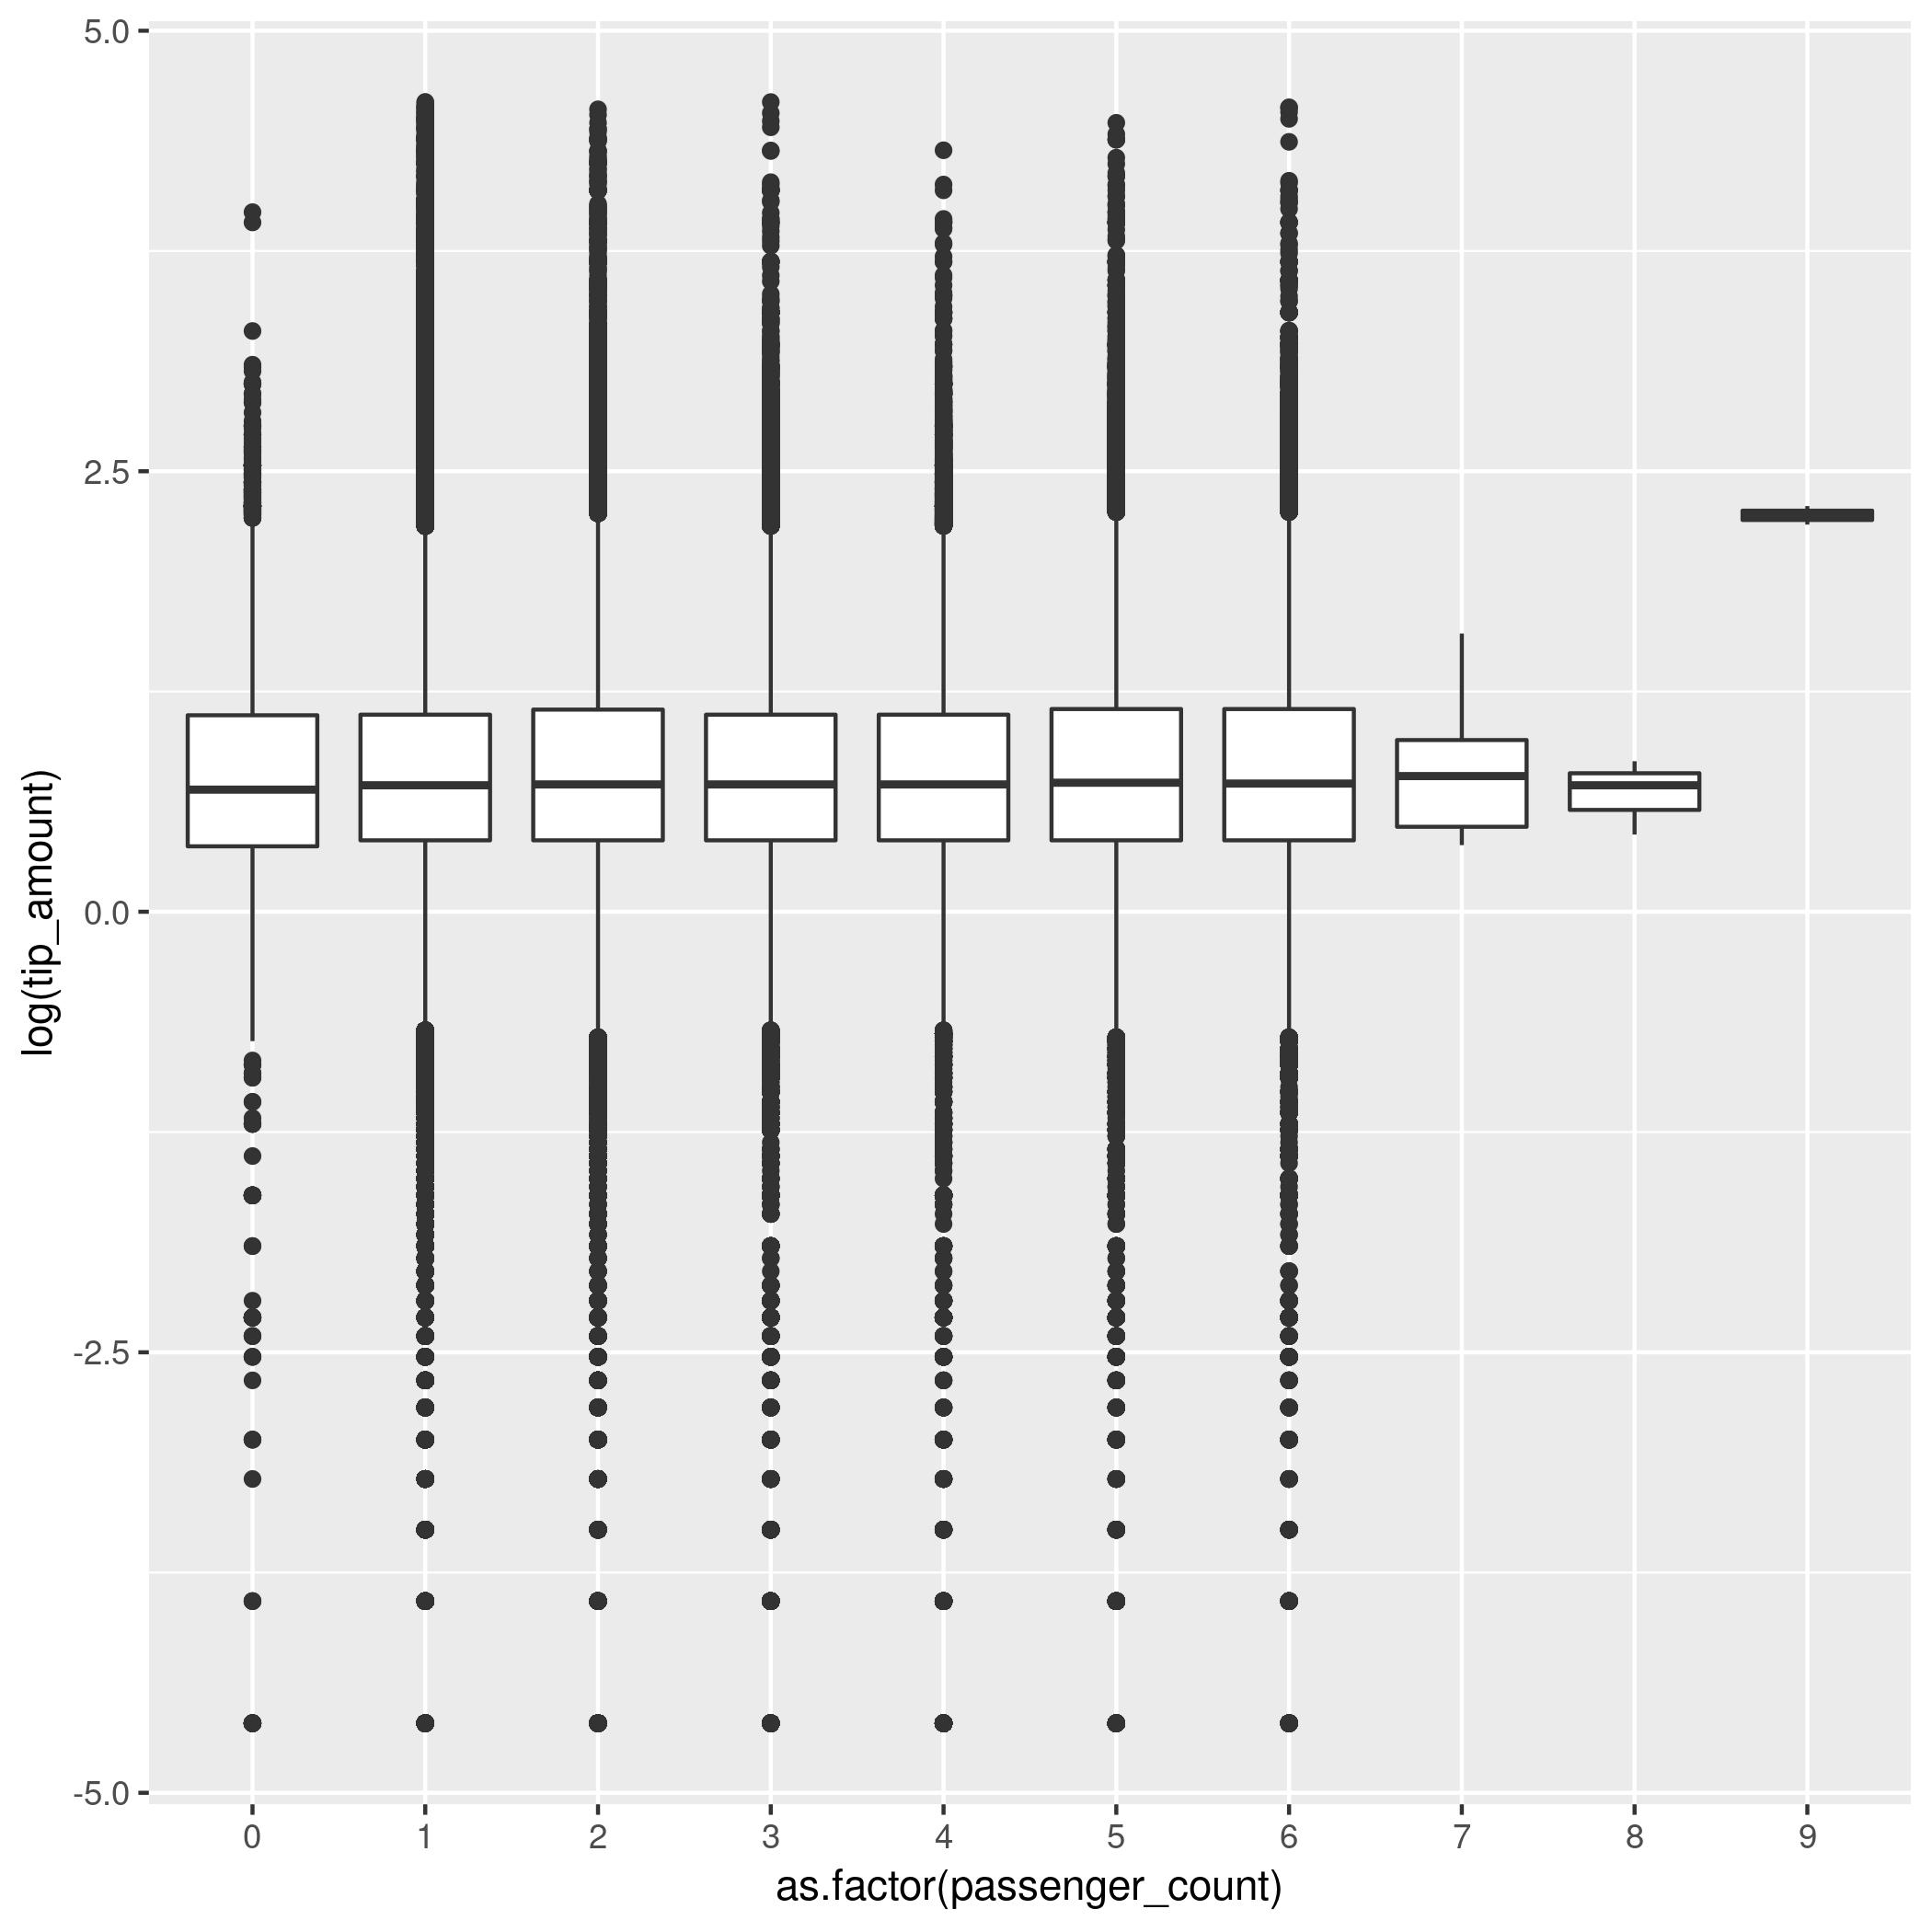
\includegraphics[width=.9\linewidth]{./plots/passengerTipBox.jpg}
\caption{\label{fig:org004926d}
Log-tip distribution by number of passengers}
\end{figure}


Next two plots display tip's distribution for the time variables computed
before. There is no noticiable difference in the tip's distribution,
other than on work days, the upper tail is fatter. These variables might
not be that interesting when modeling.
\begin{figure}[htbp]
\centering
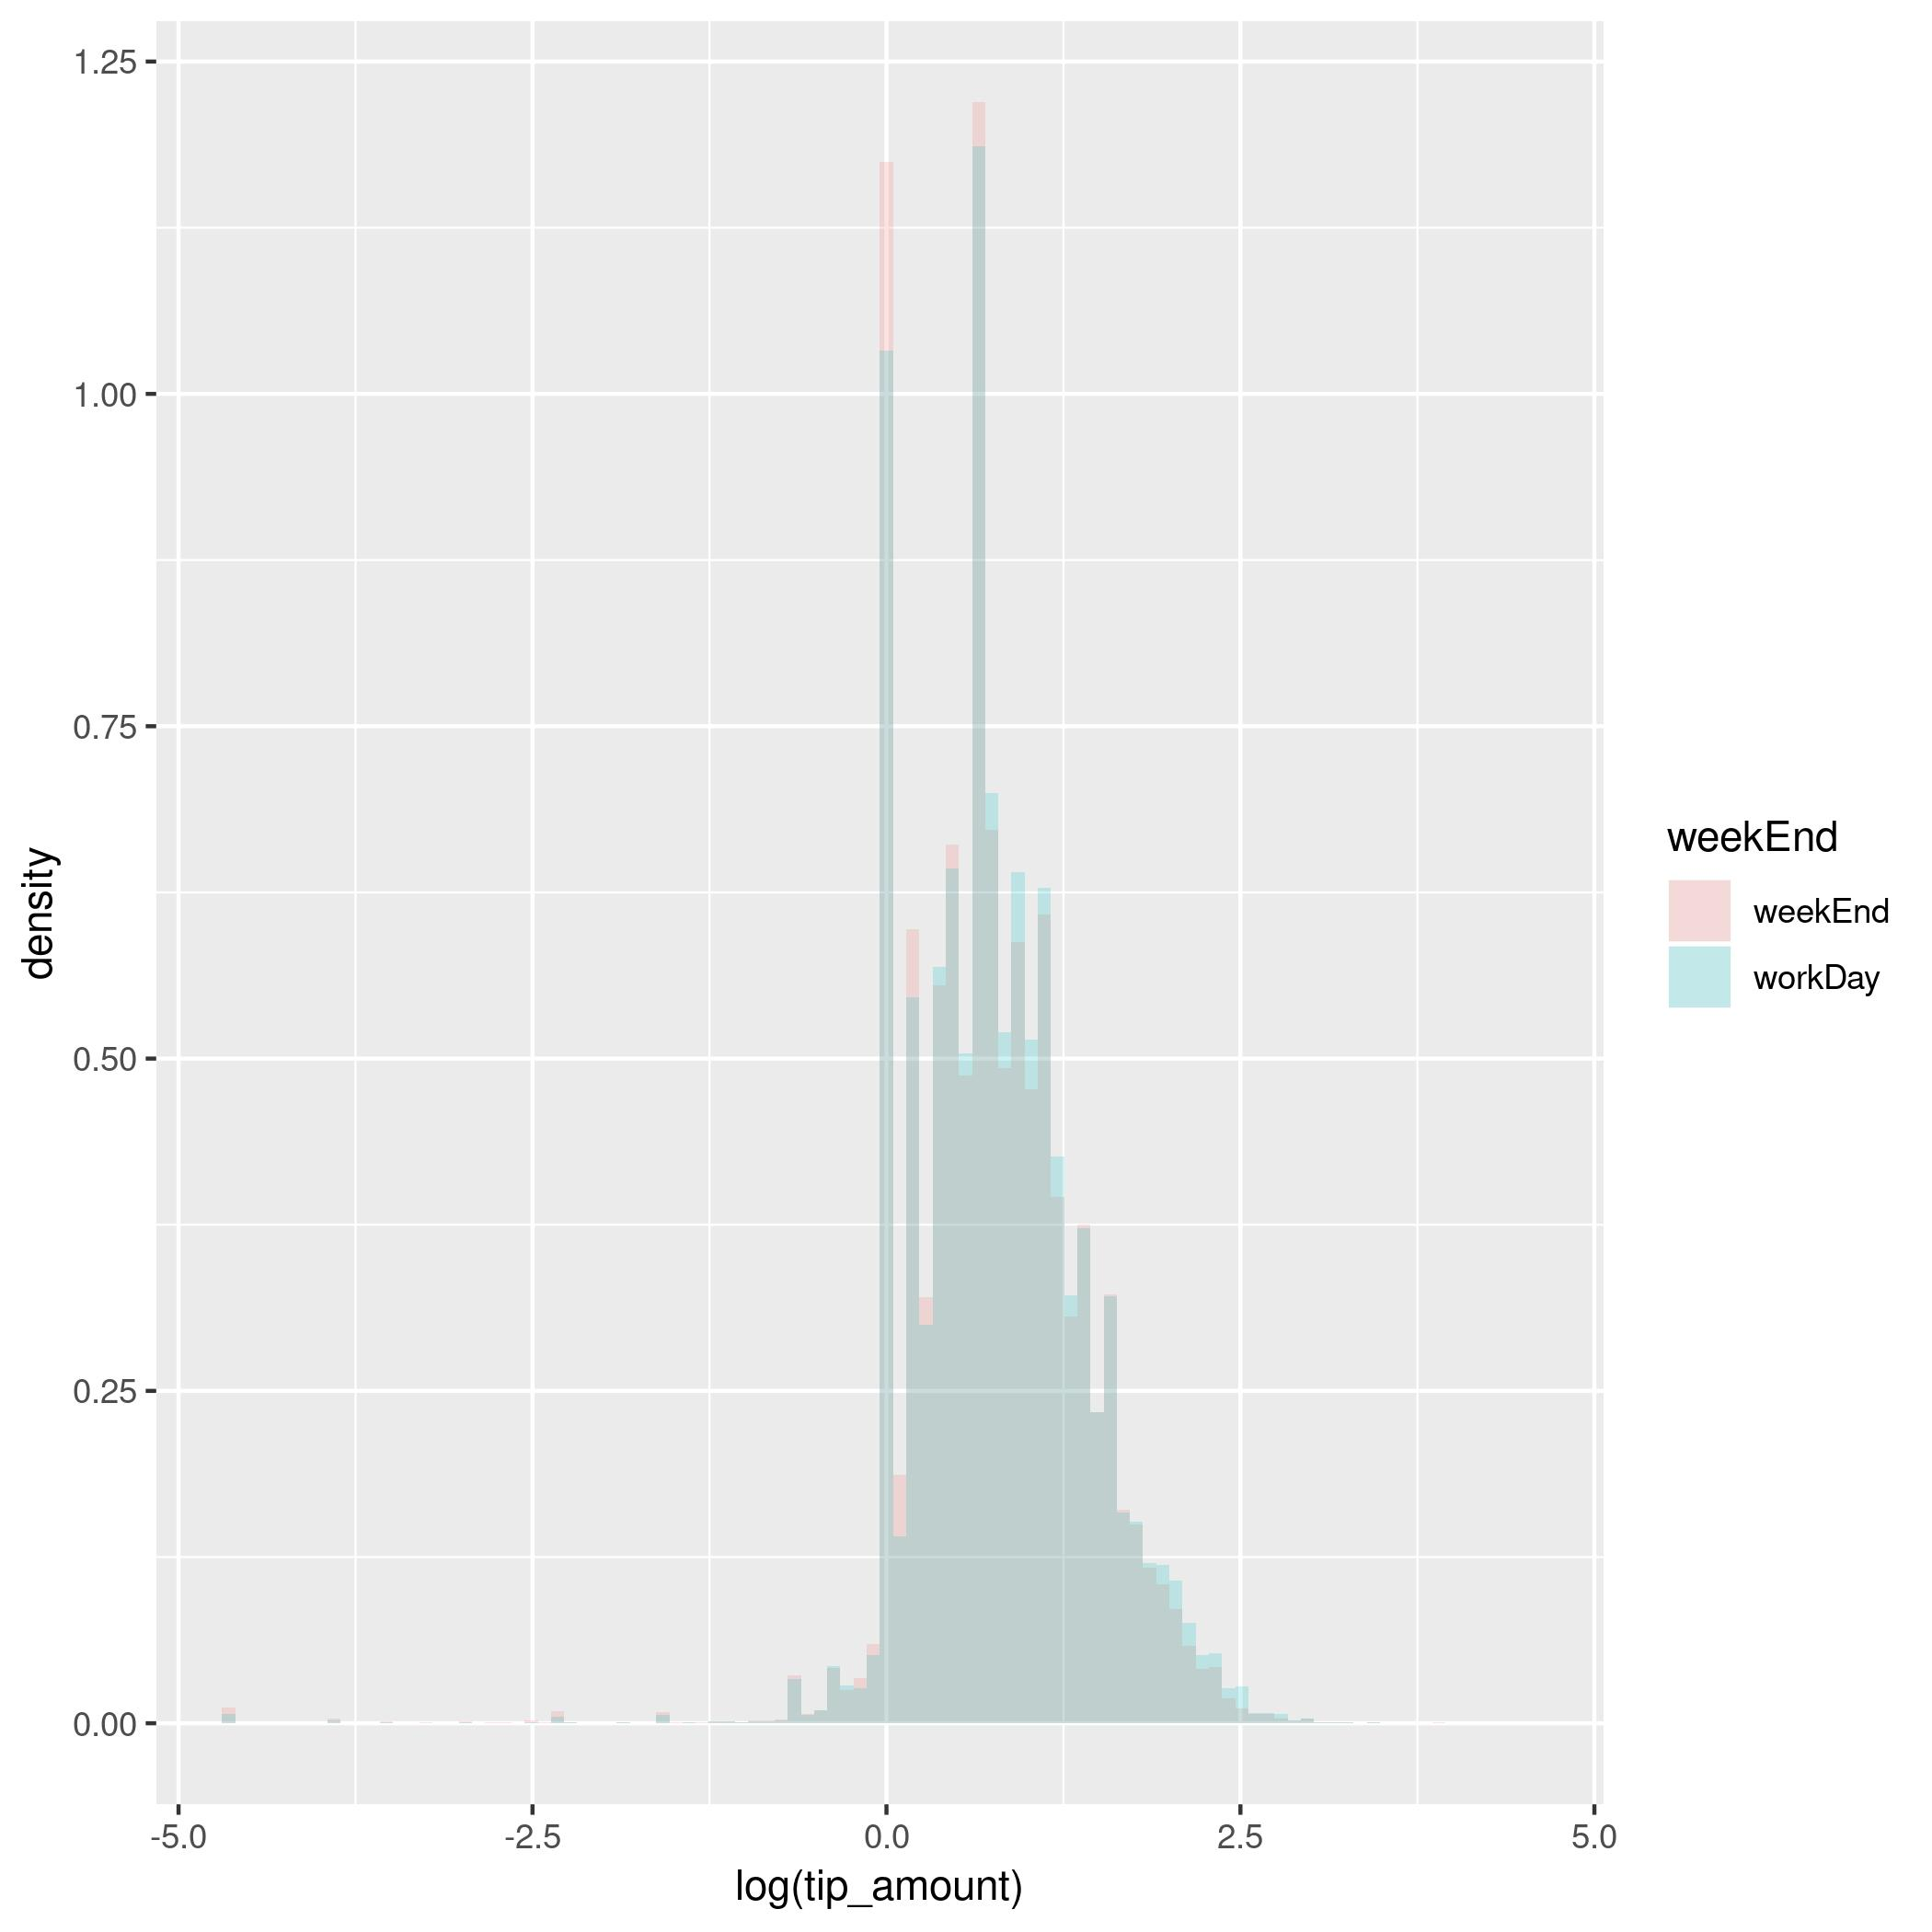
\includegraphics[width=.9\linewidth]{./plots/weekendTipDensityHist.jpg}
\caption{\label{fig:org2dc1a4d}
Log-tip density histogram by day type}
\end{figure}


\begin{figure}[htbp]
\centering
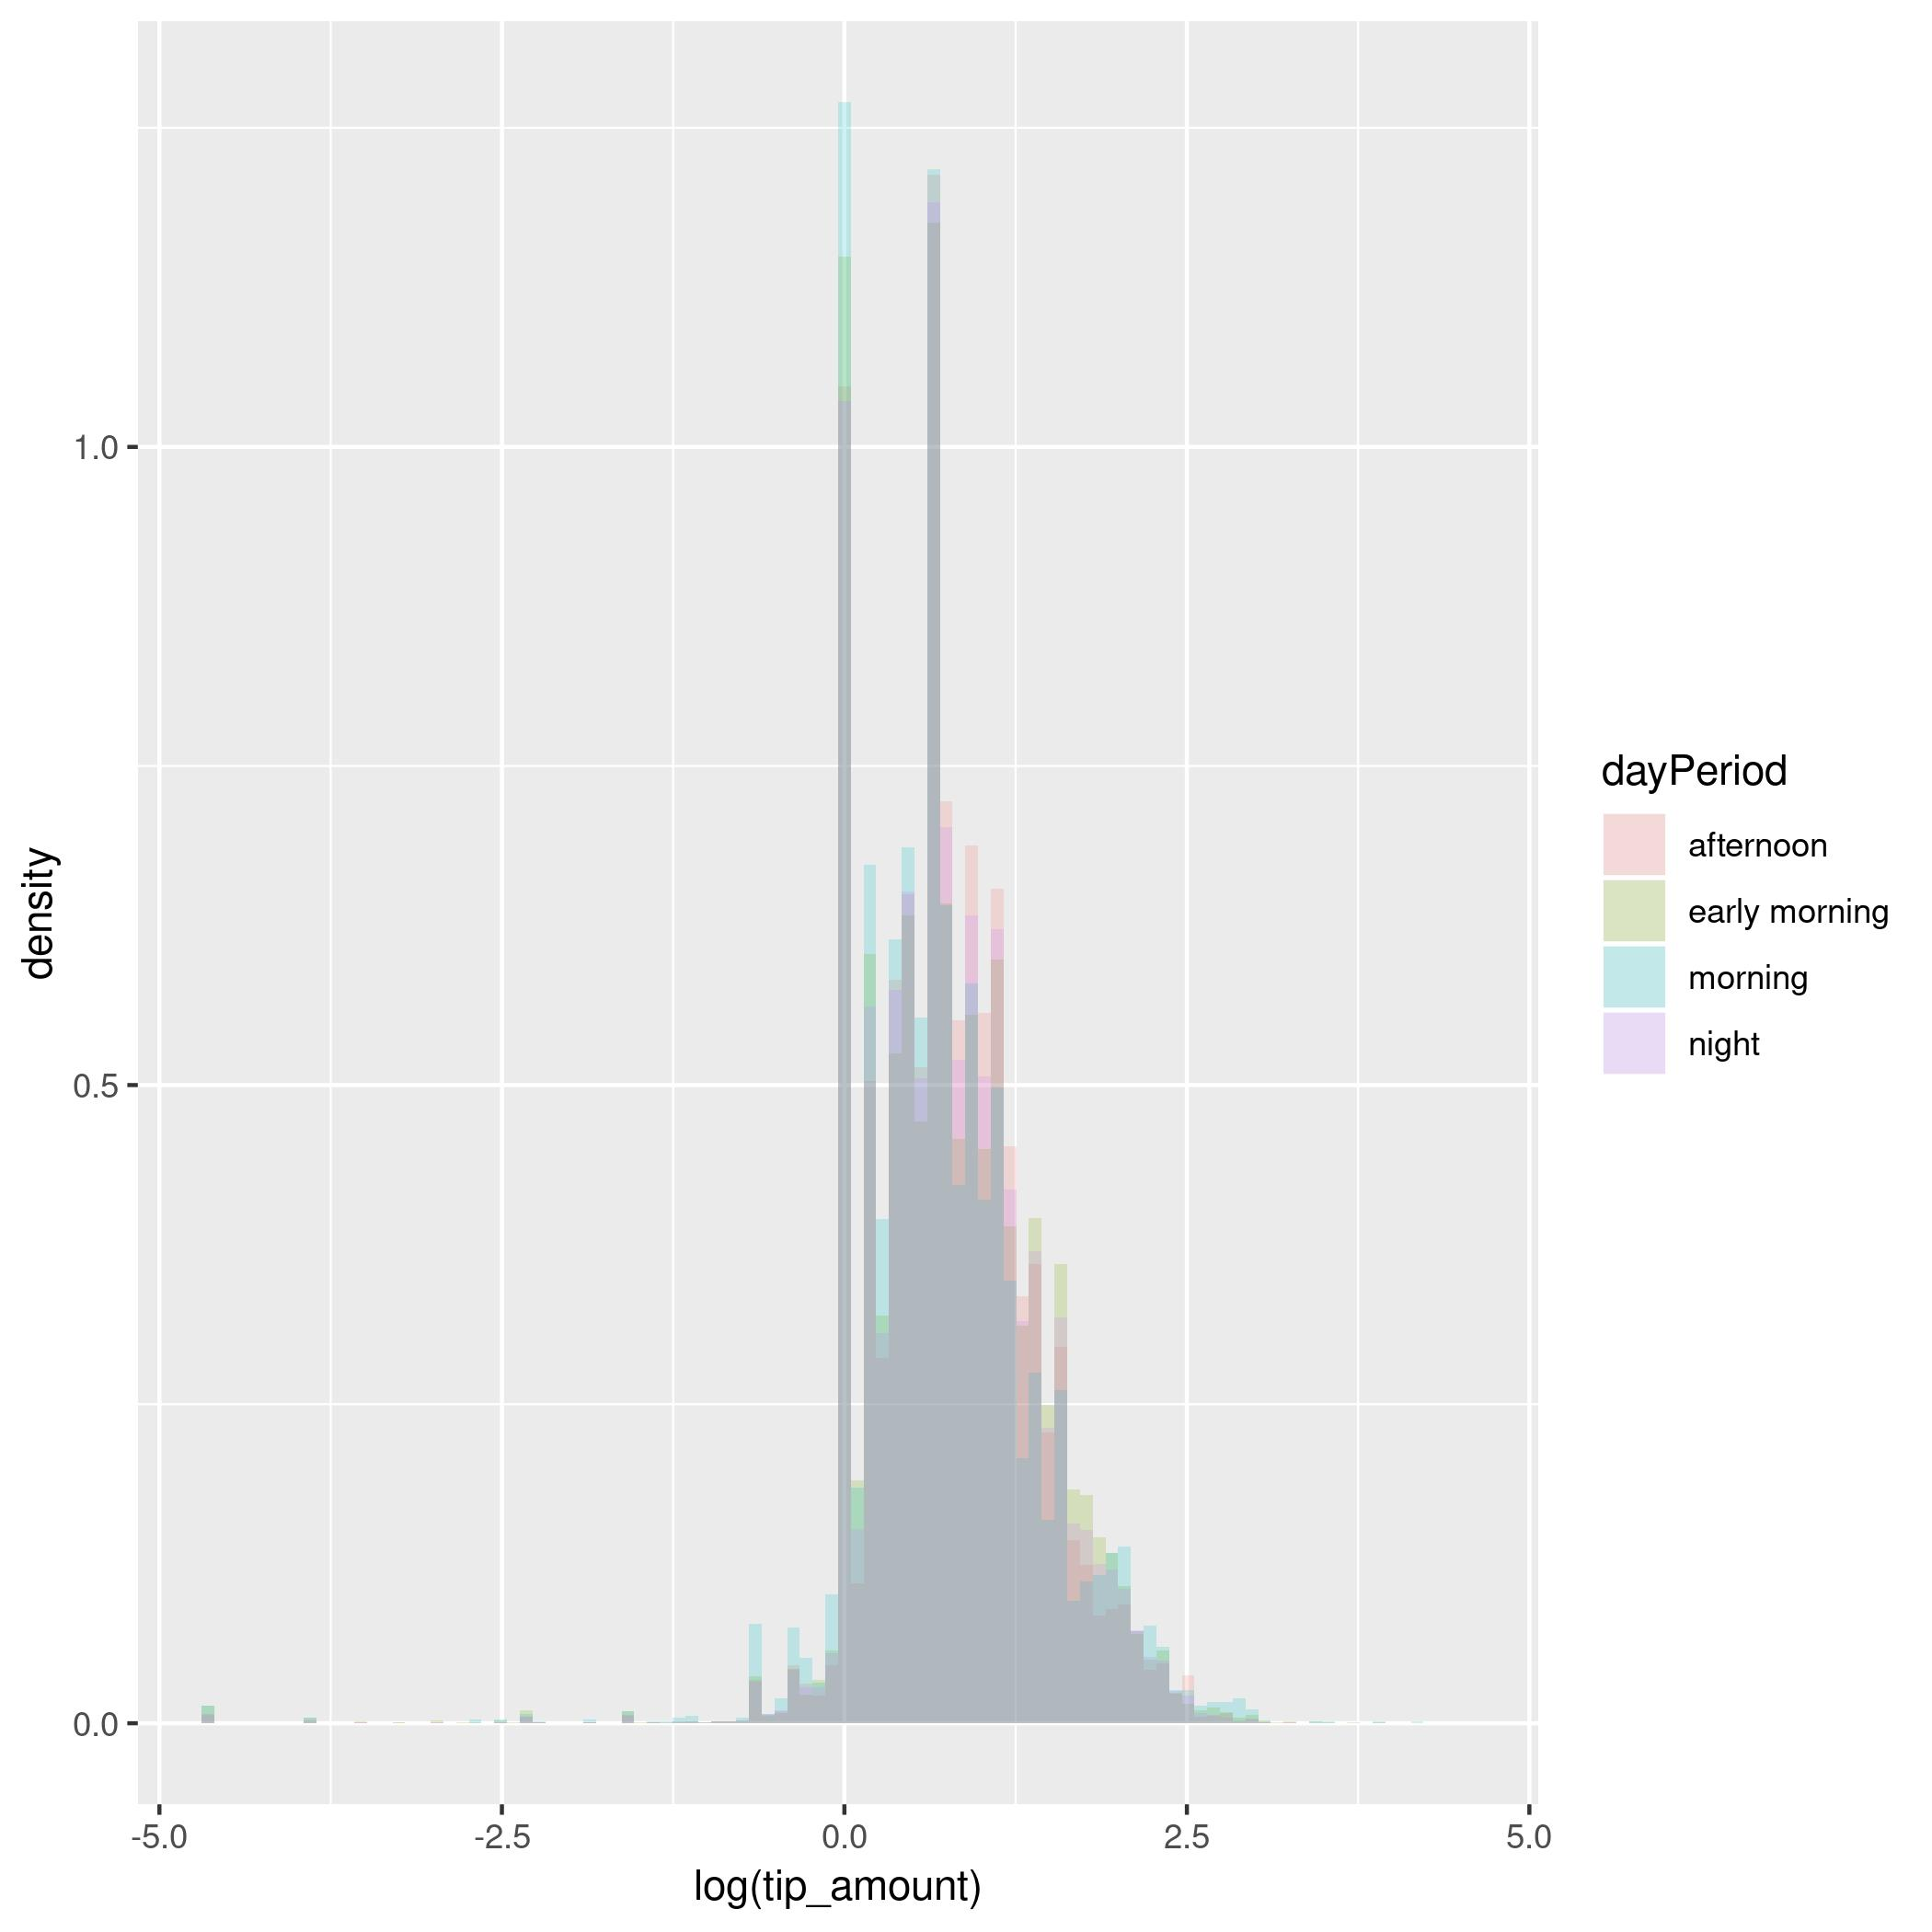
\includegraphics[width=.9\linewidth]{./plots/dayPeriodTipDensityHist.jpg}
\caption{\label{fig:org53e1af9}
Log-tip density histogram by time of the day}
\end{figure}

Next plot displays tip's density by each of the payment types.
People paying cash (coded as 2) seem to always give a \$1 tip.
Given the little amount of customers not using credit card, this
variable will not be used in the model.

\begin{figure}[htbp]
\centering
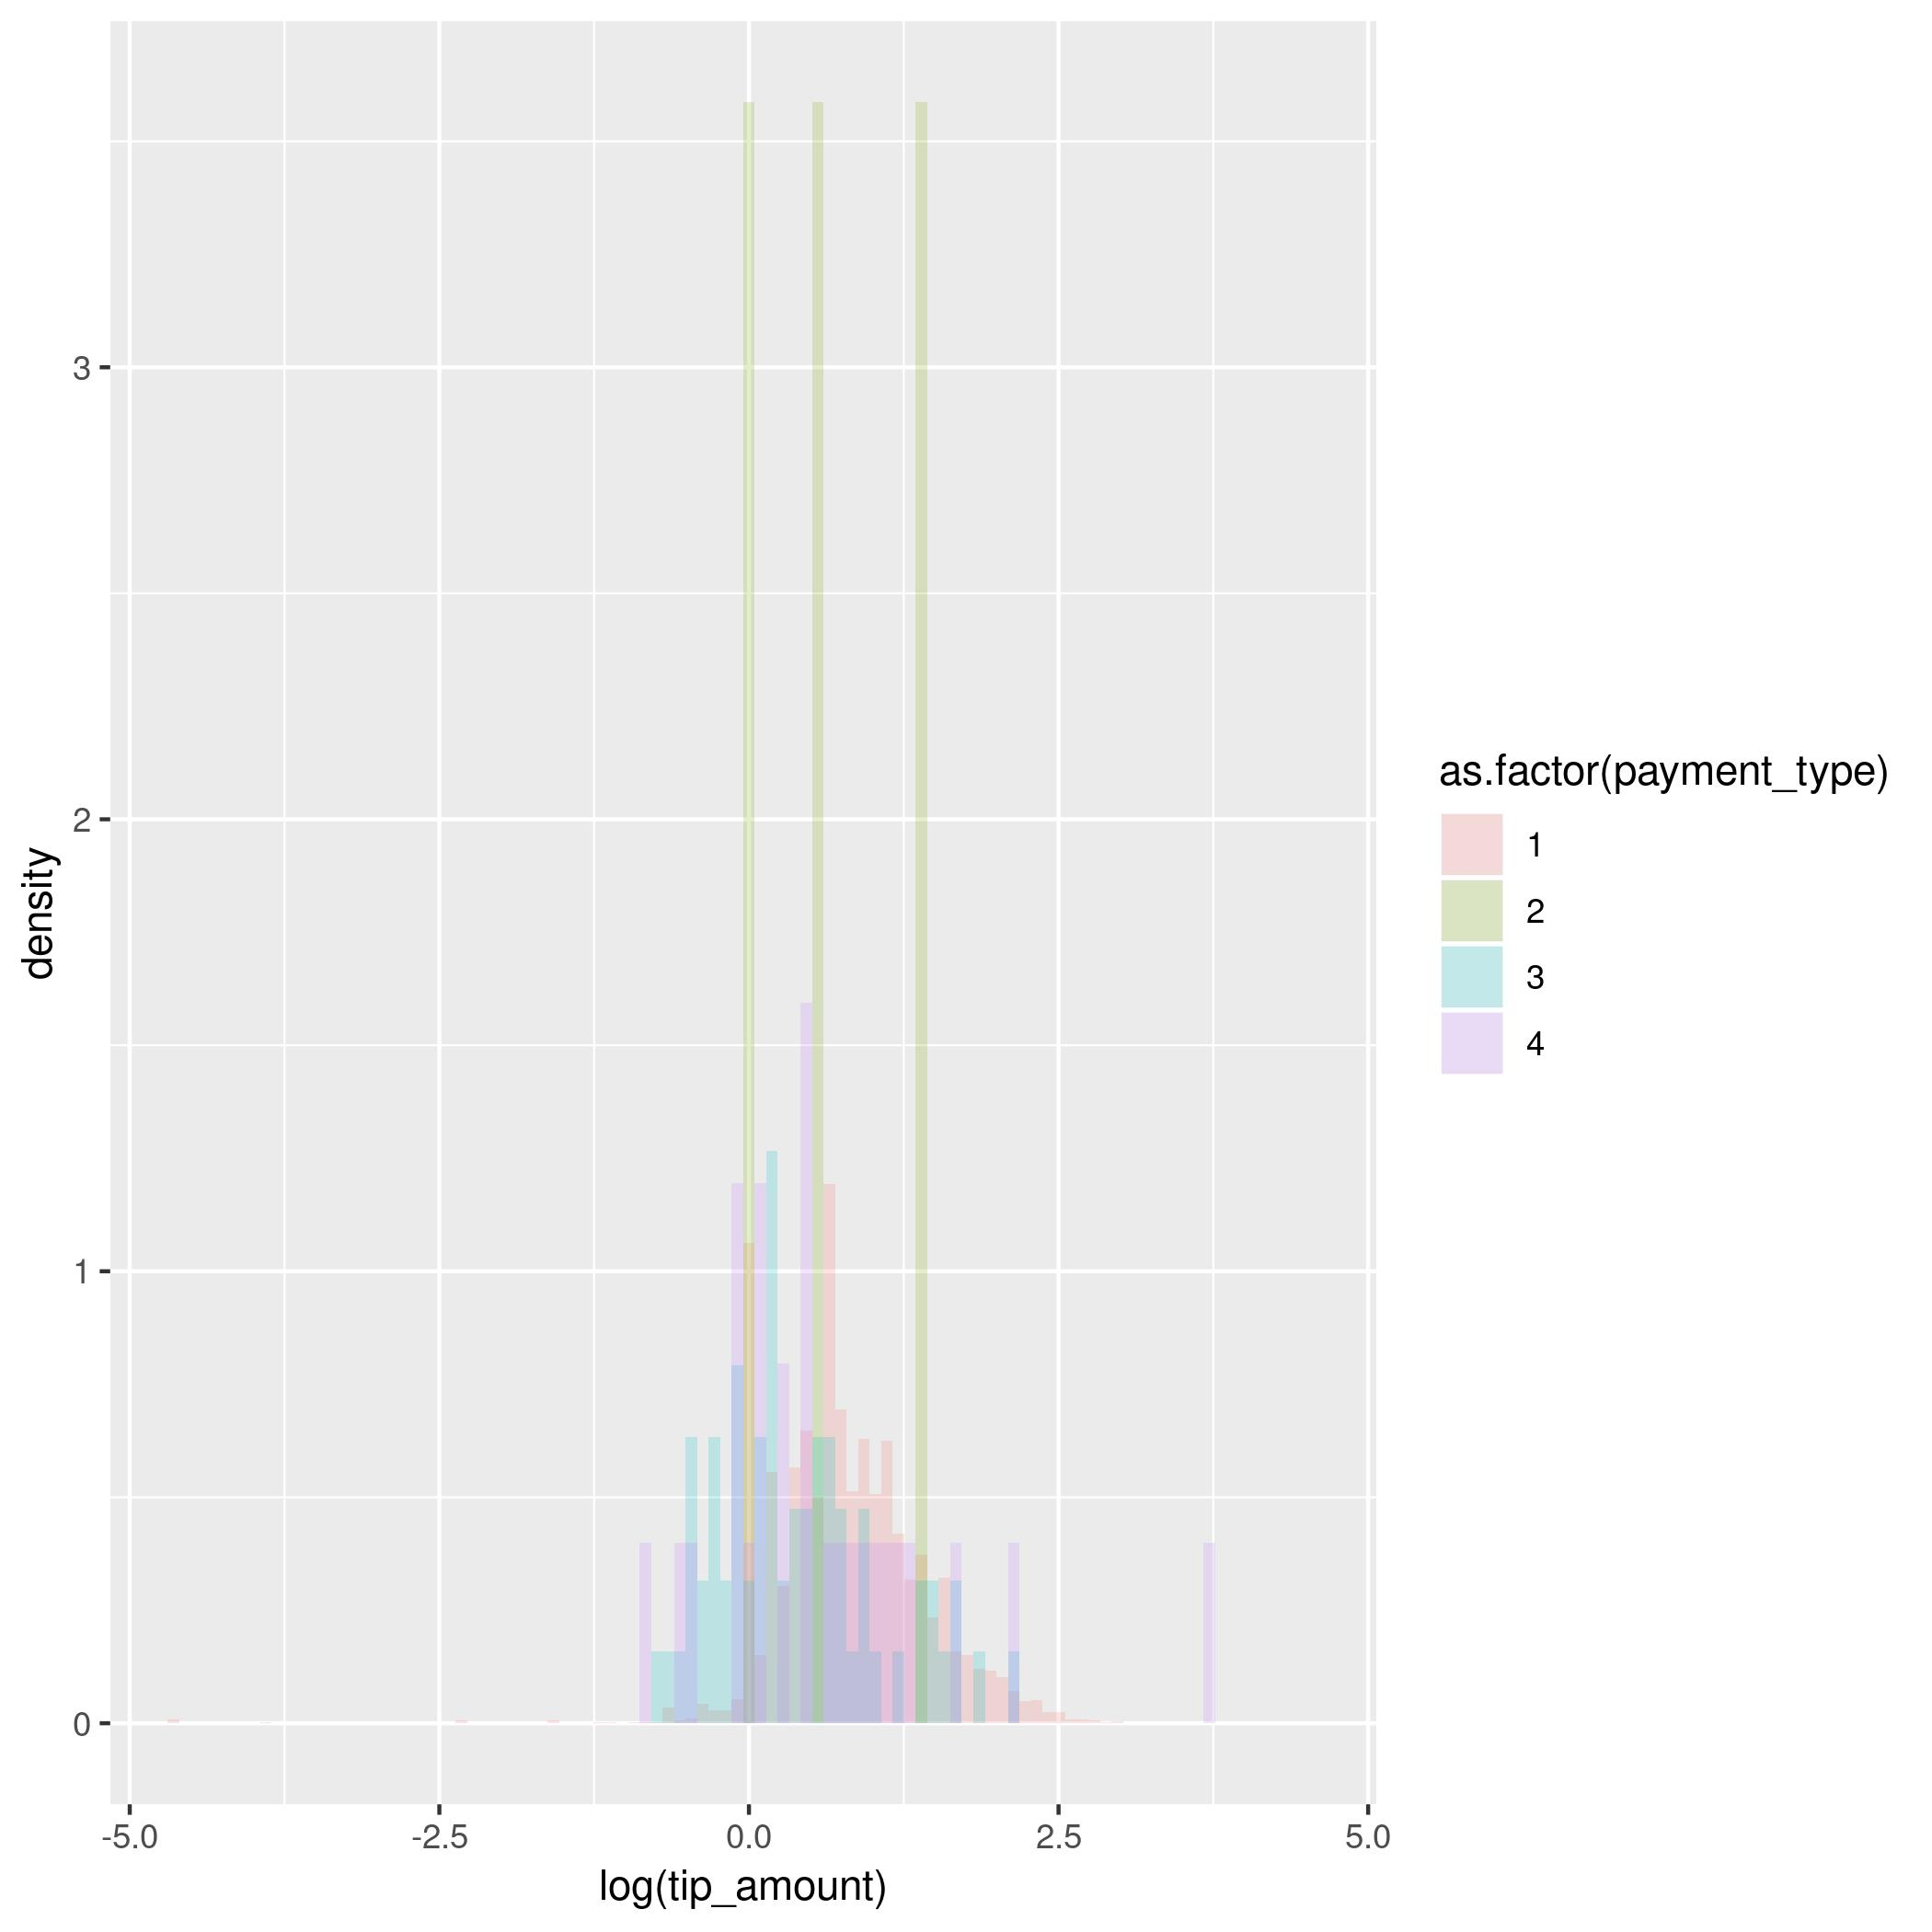
\includegraphics[width=.9\linewidth]{./plots/paymentTipDensityHist.jpg}
\caption{\label{fig:org99cbaa0}
Log-tip density histogram by payment type}
\end{figure}

Next plot displays tip's density on the cases where, as far as I have
understood, the driver was asked to wait somewhere mid ride.
In this case, when the driver was asked to wait, there is a noticeable
bimodality in the tips given. This is an interesting property.
\begin{figure}[htbp]
\centering
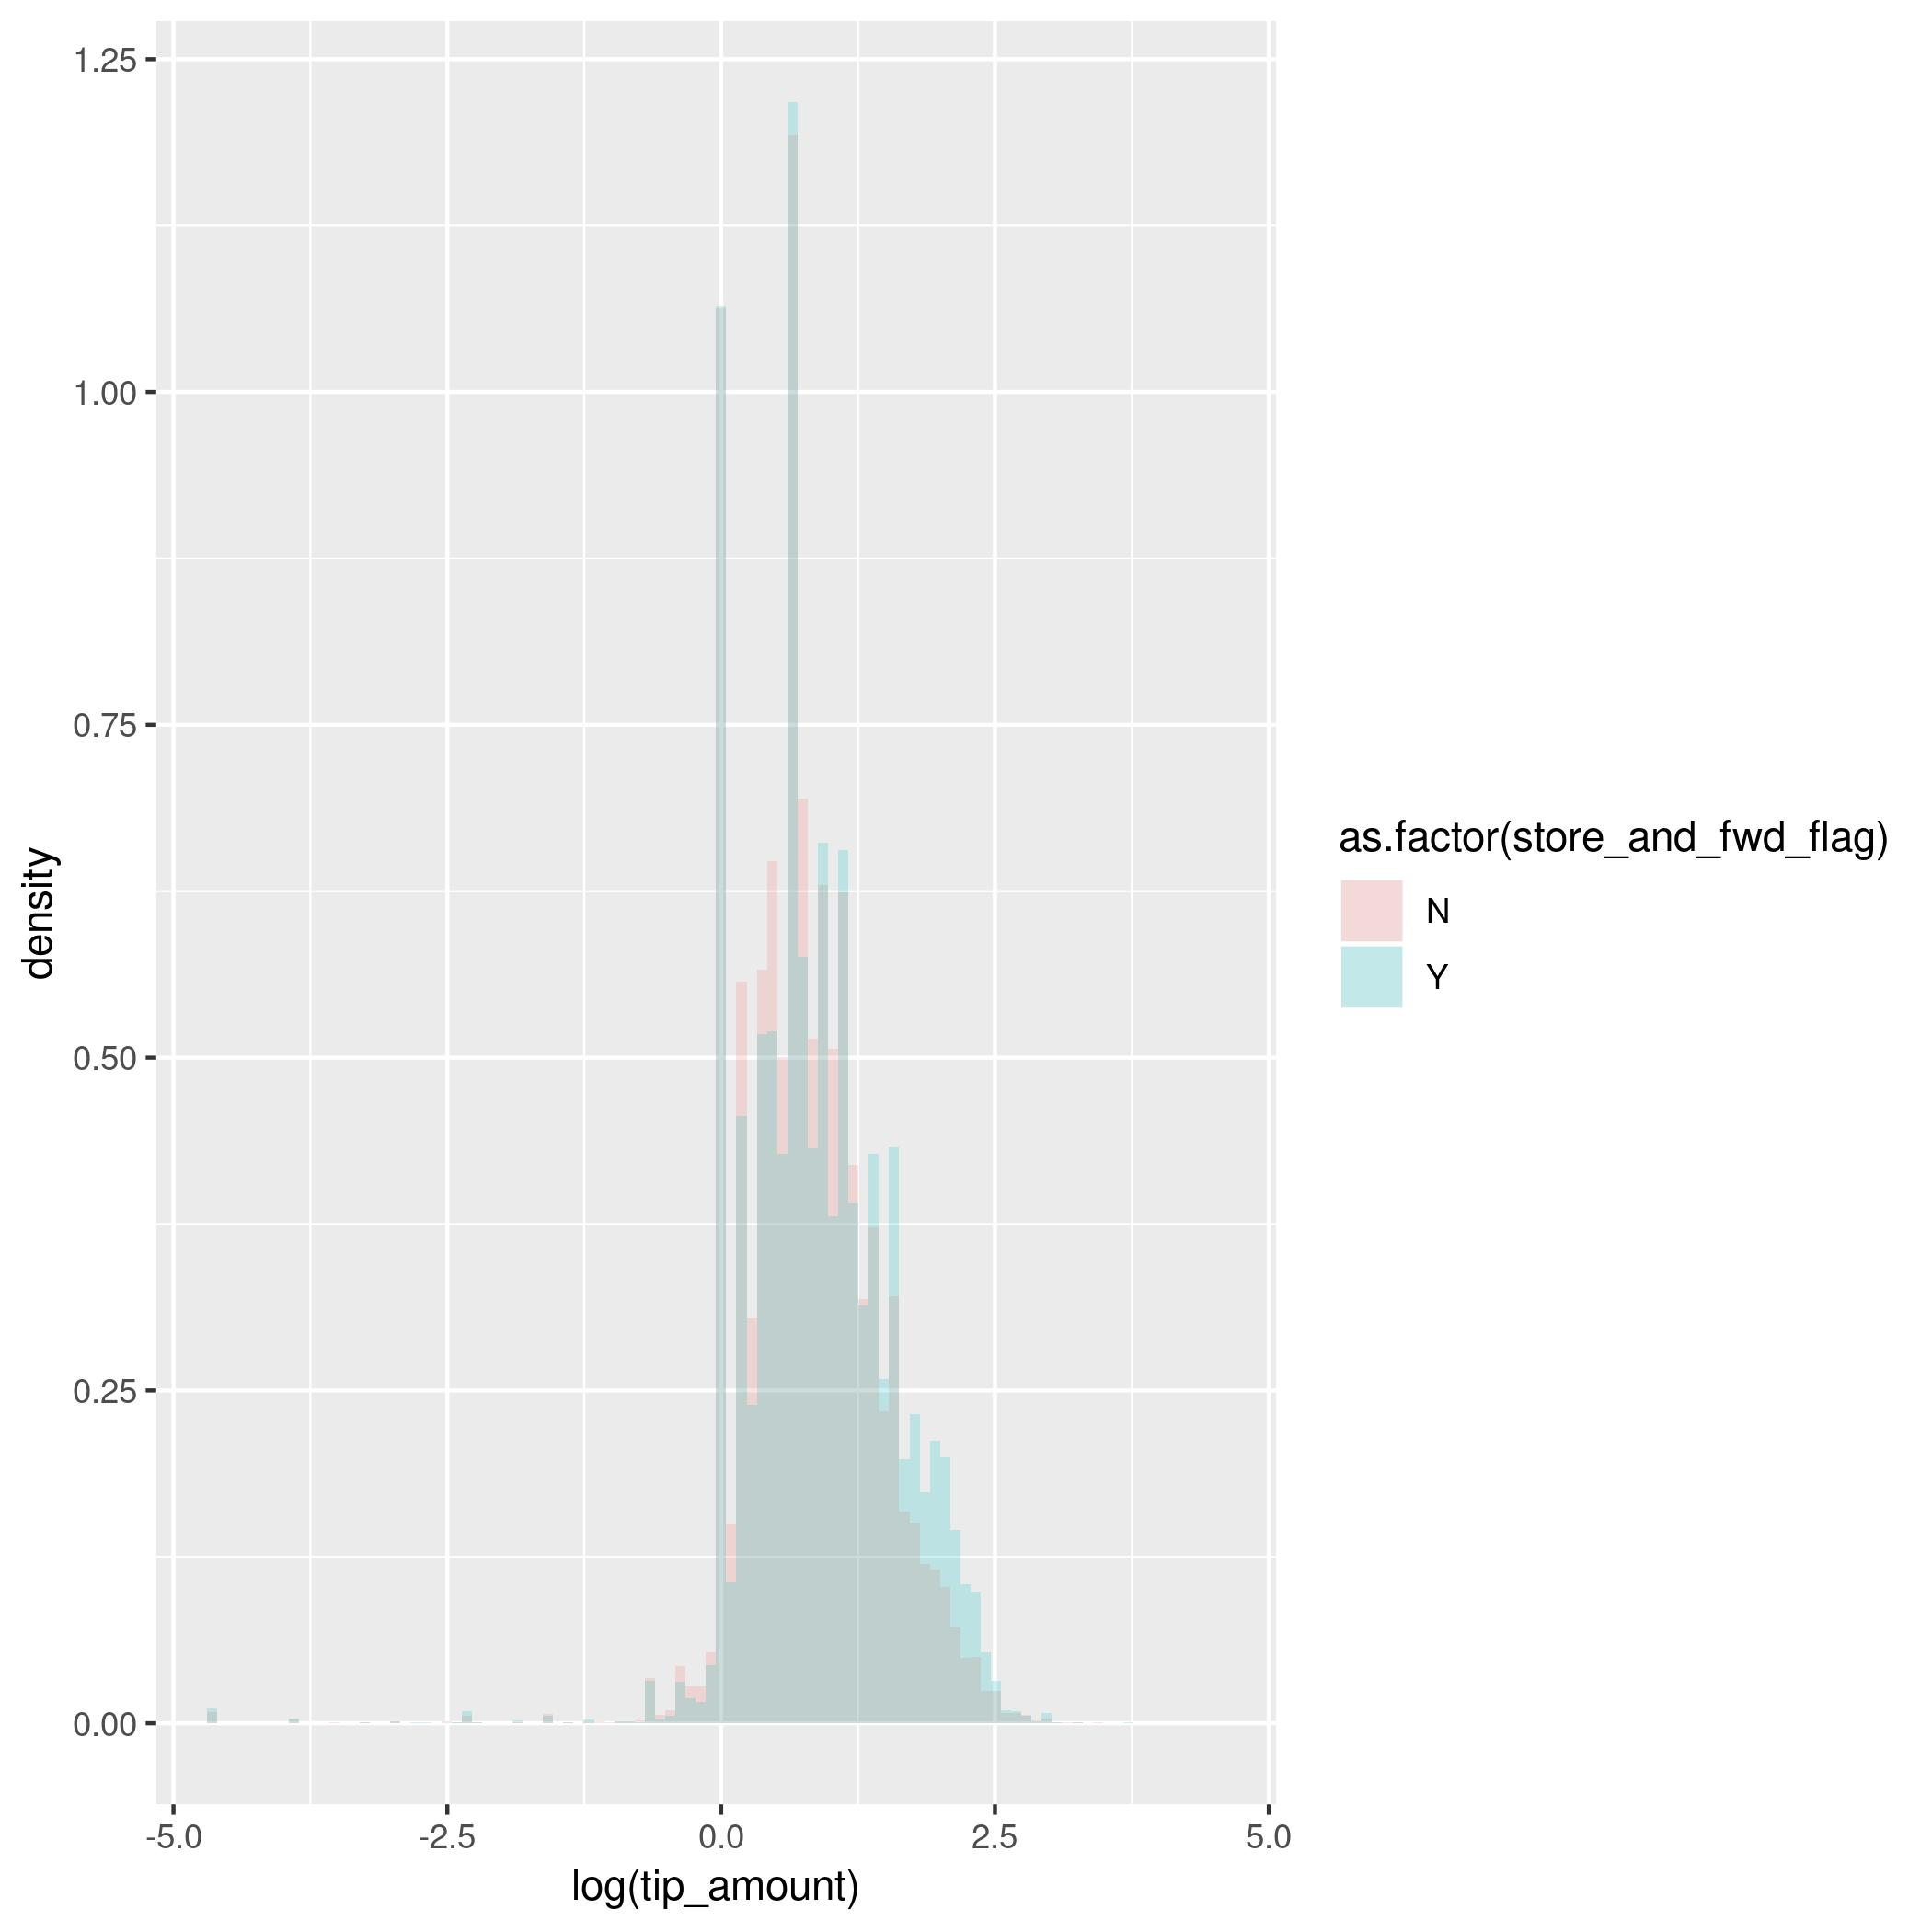
\includegraphics[width=.9\linewidth]{./plots/storeCodeTipDensityHist.jpg}
\caption{\label{fig:org4c29f79}
Log-tip density histogram by store flag}
\end{figure}

Next plot displays tip's density for each of the rate codes.
When this variable is set to 1, the standard rate applies, other
cases are trips involving either airports or outer neighborhoods of
the city. there is a noticeable difference in the distribution between
the standard rate and all others.
\begin{figure}[htbp]
\centering
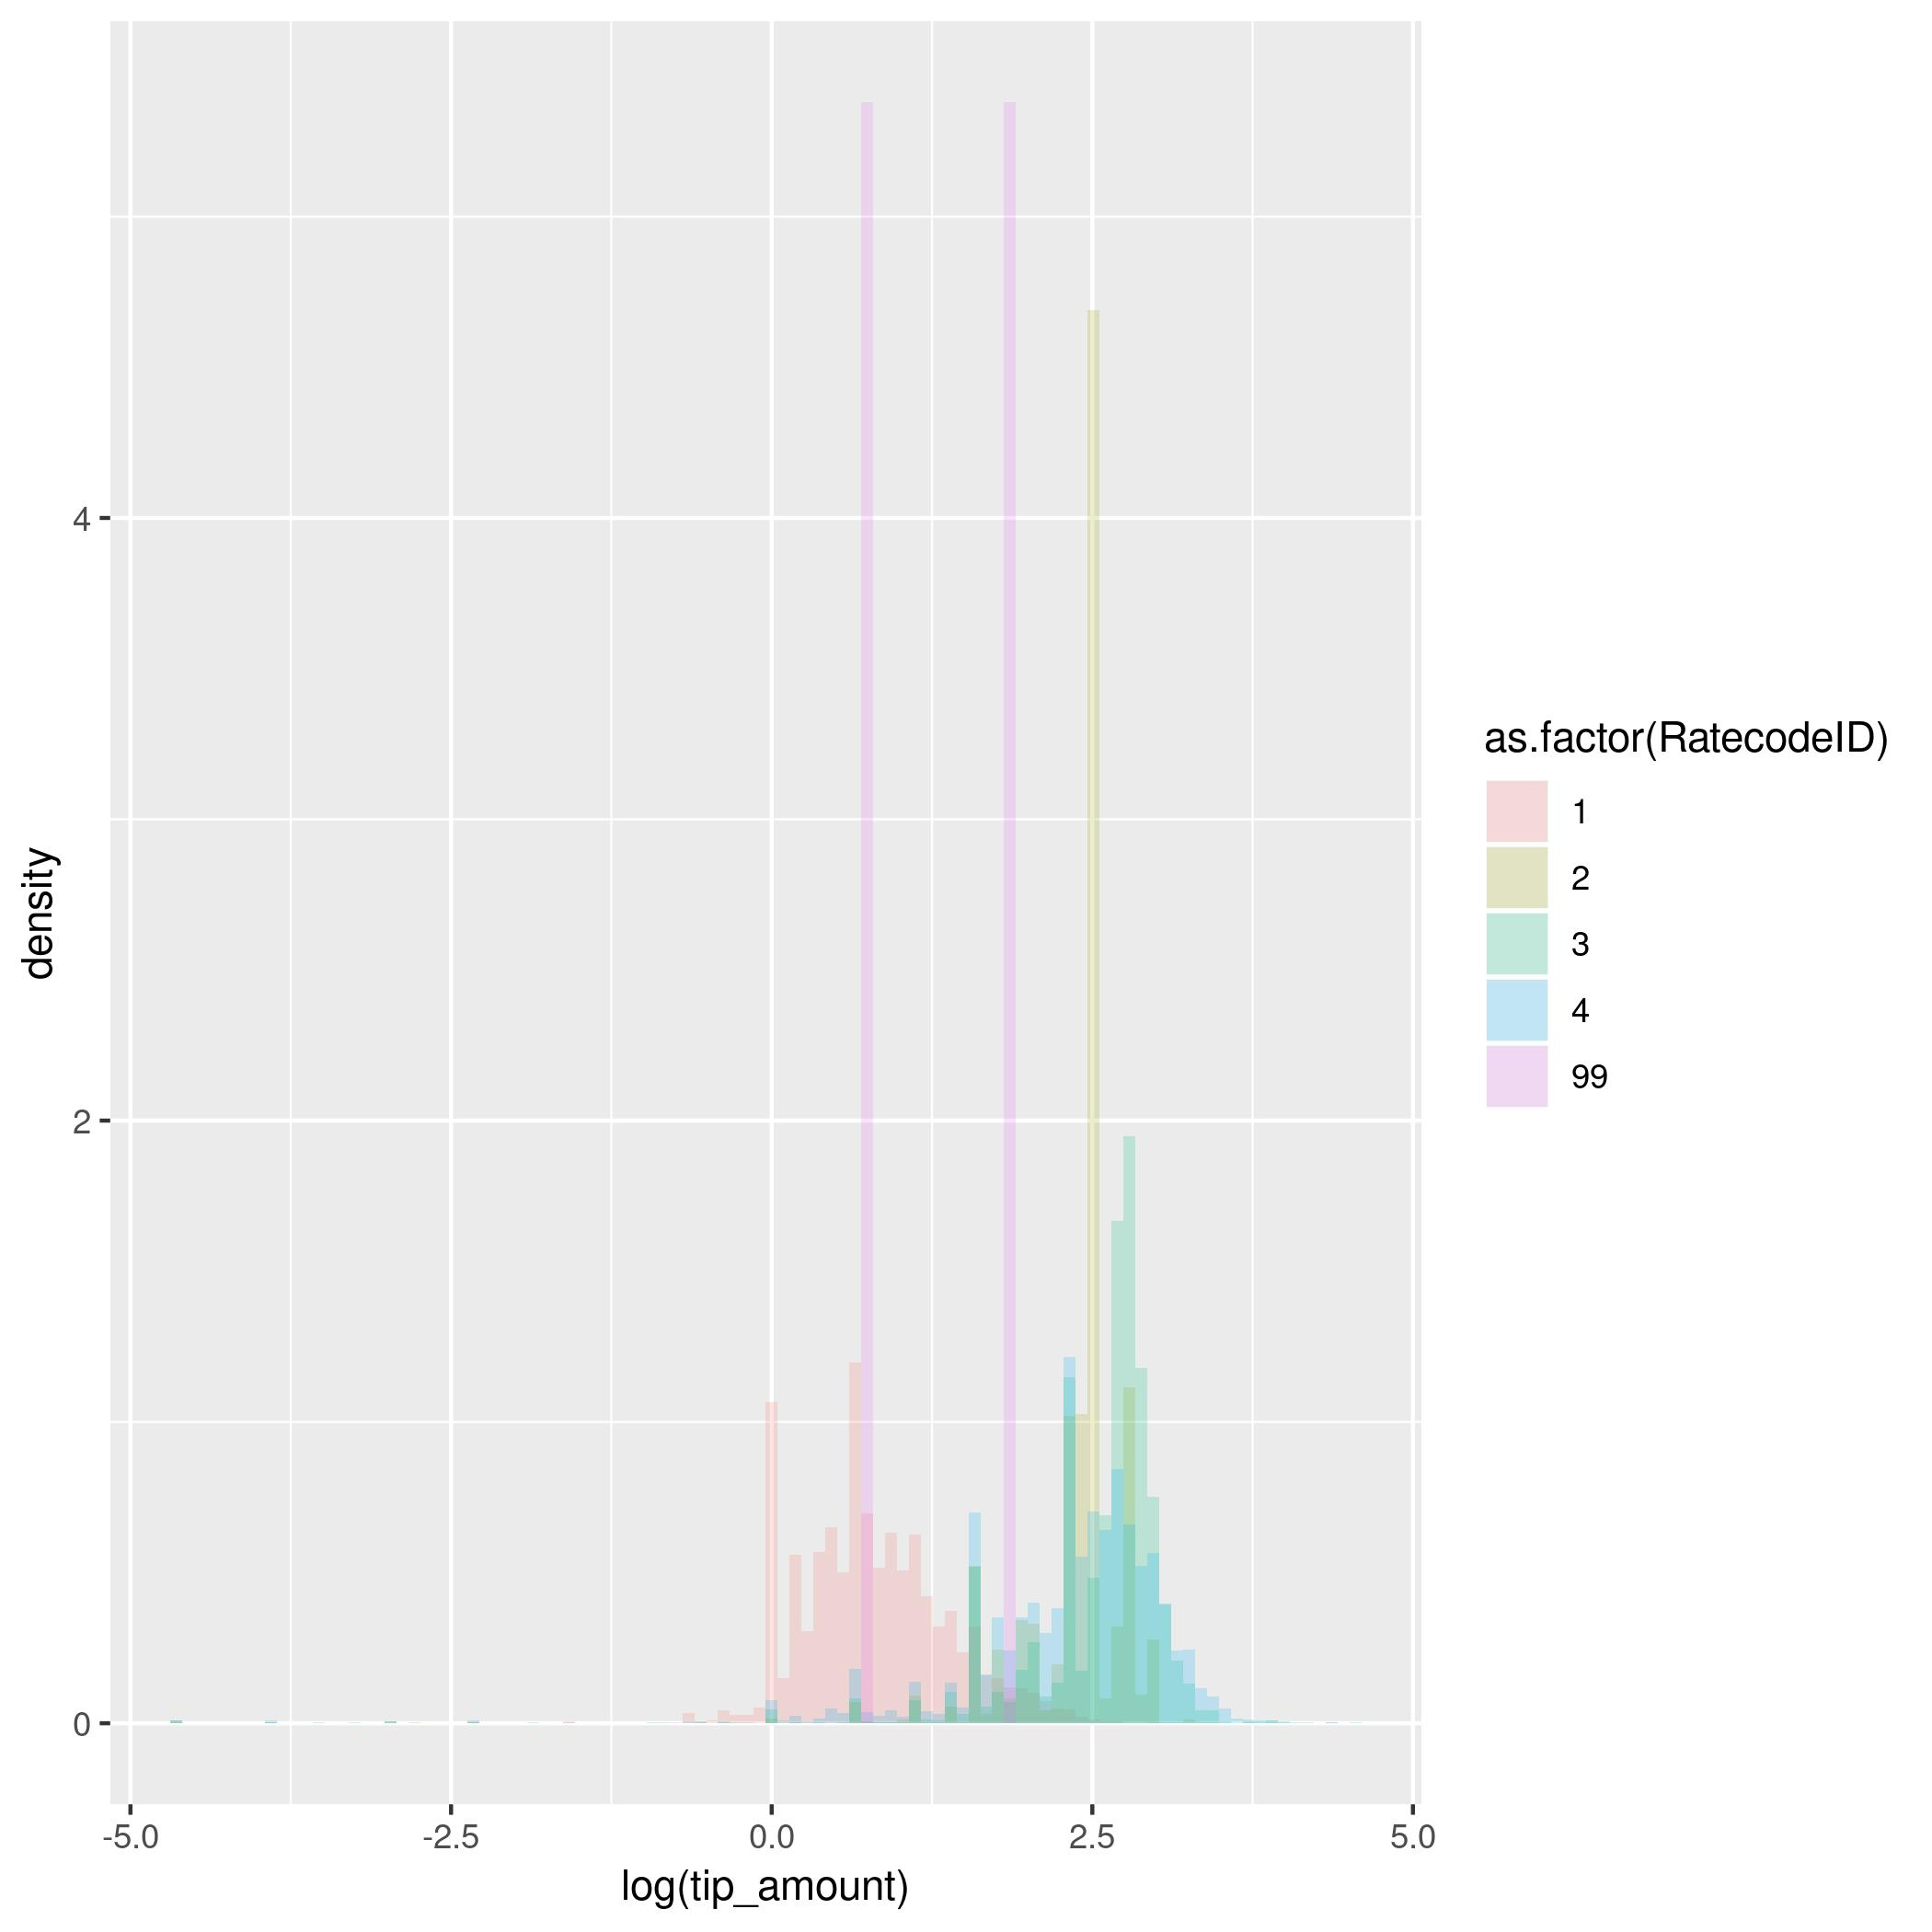
\includegraphics[width=.9\linewidth]{./plots/rateCodeTipDensityHist.jpg}
\caption{\label{fig:org4240786}
Log-tip density histogram by rate type}
\end{figure}


Next two plots help understand tip's relation with \emph{trip\_distance}.
First we look at the log-trip-distance histogram.
\begin{figure}[htbp]
\centering
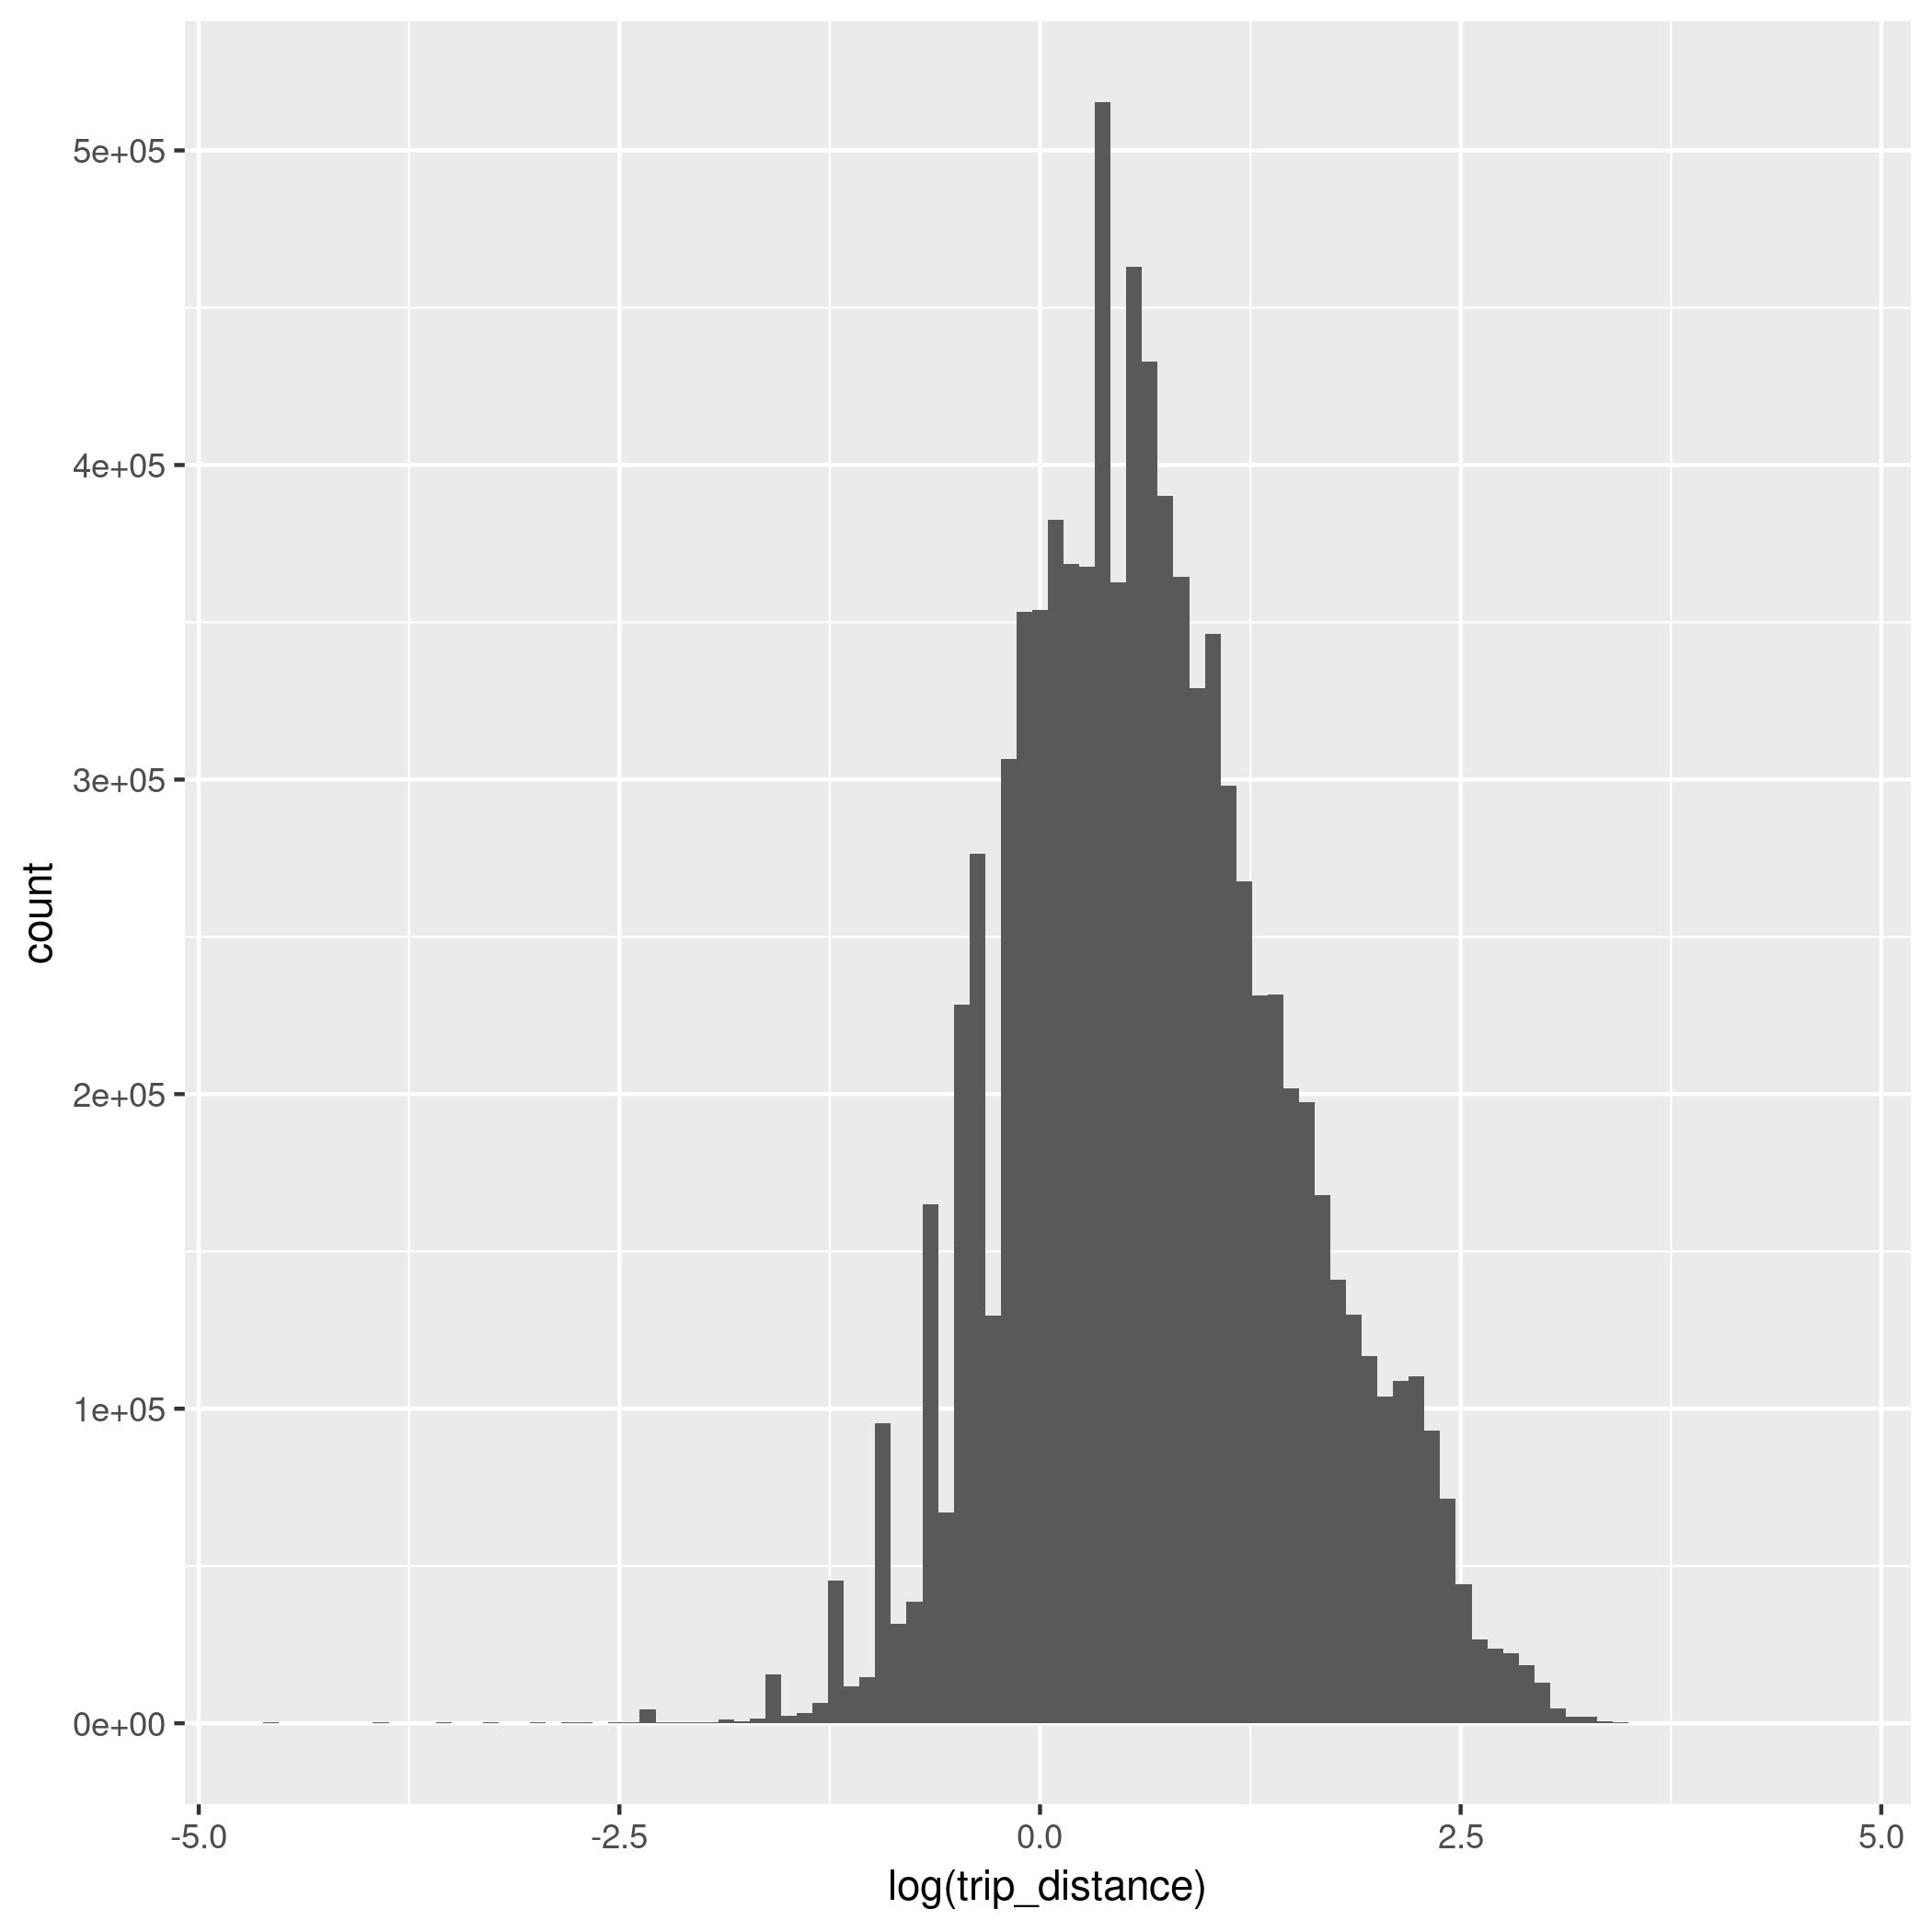
\includegraphics[width=.9\linewidth]{./plots/logTripDistanceHist.jpg}
\caption{\label{fig:orge5fda18}
Log-trip\_distance histogram}
\end{figure}

Second we look at the log-tip vs log-distance, and notice strong
positive correlation.
\begin{figure}[htbp]
\centering
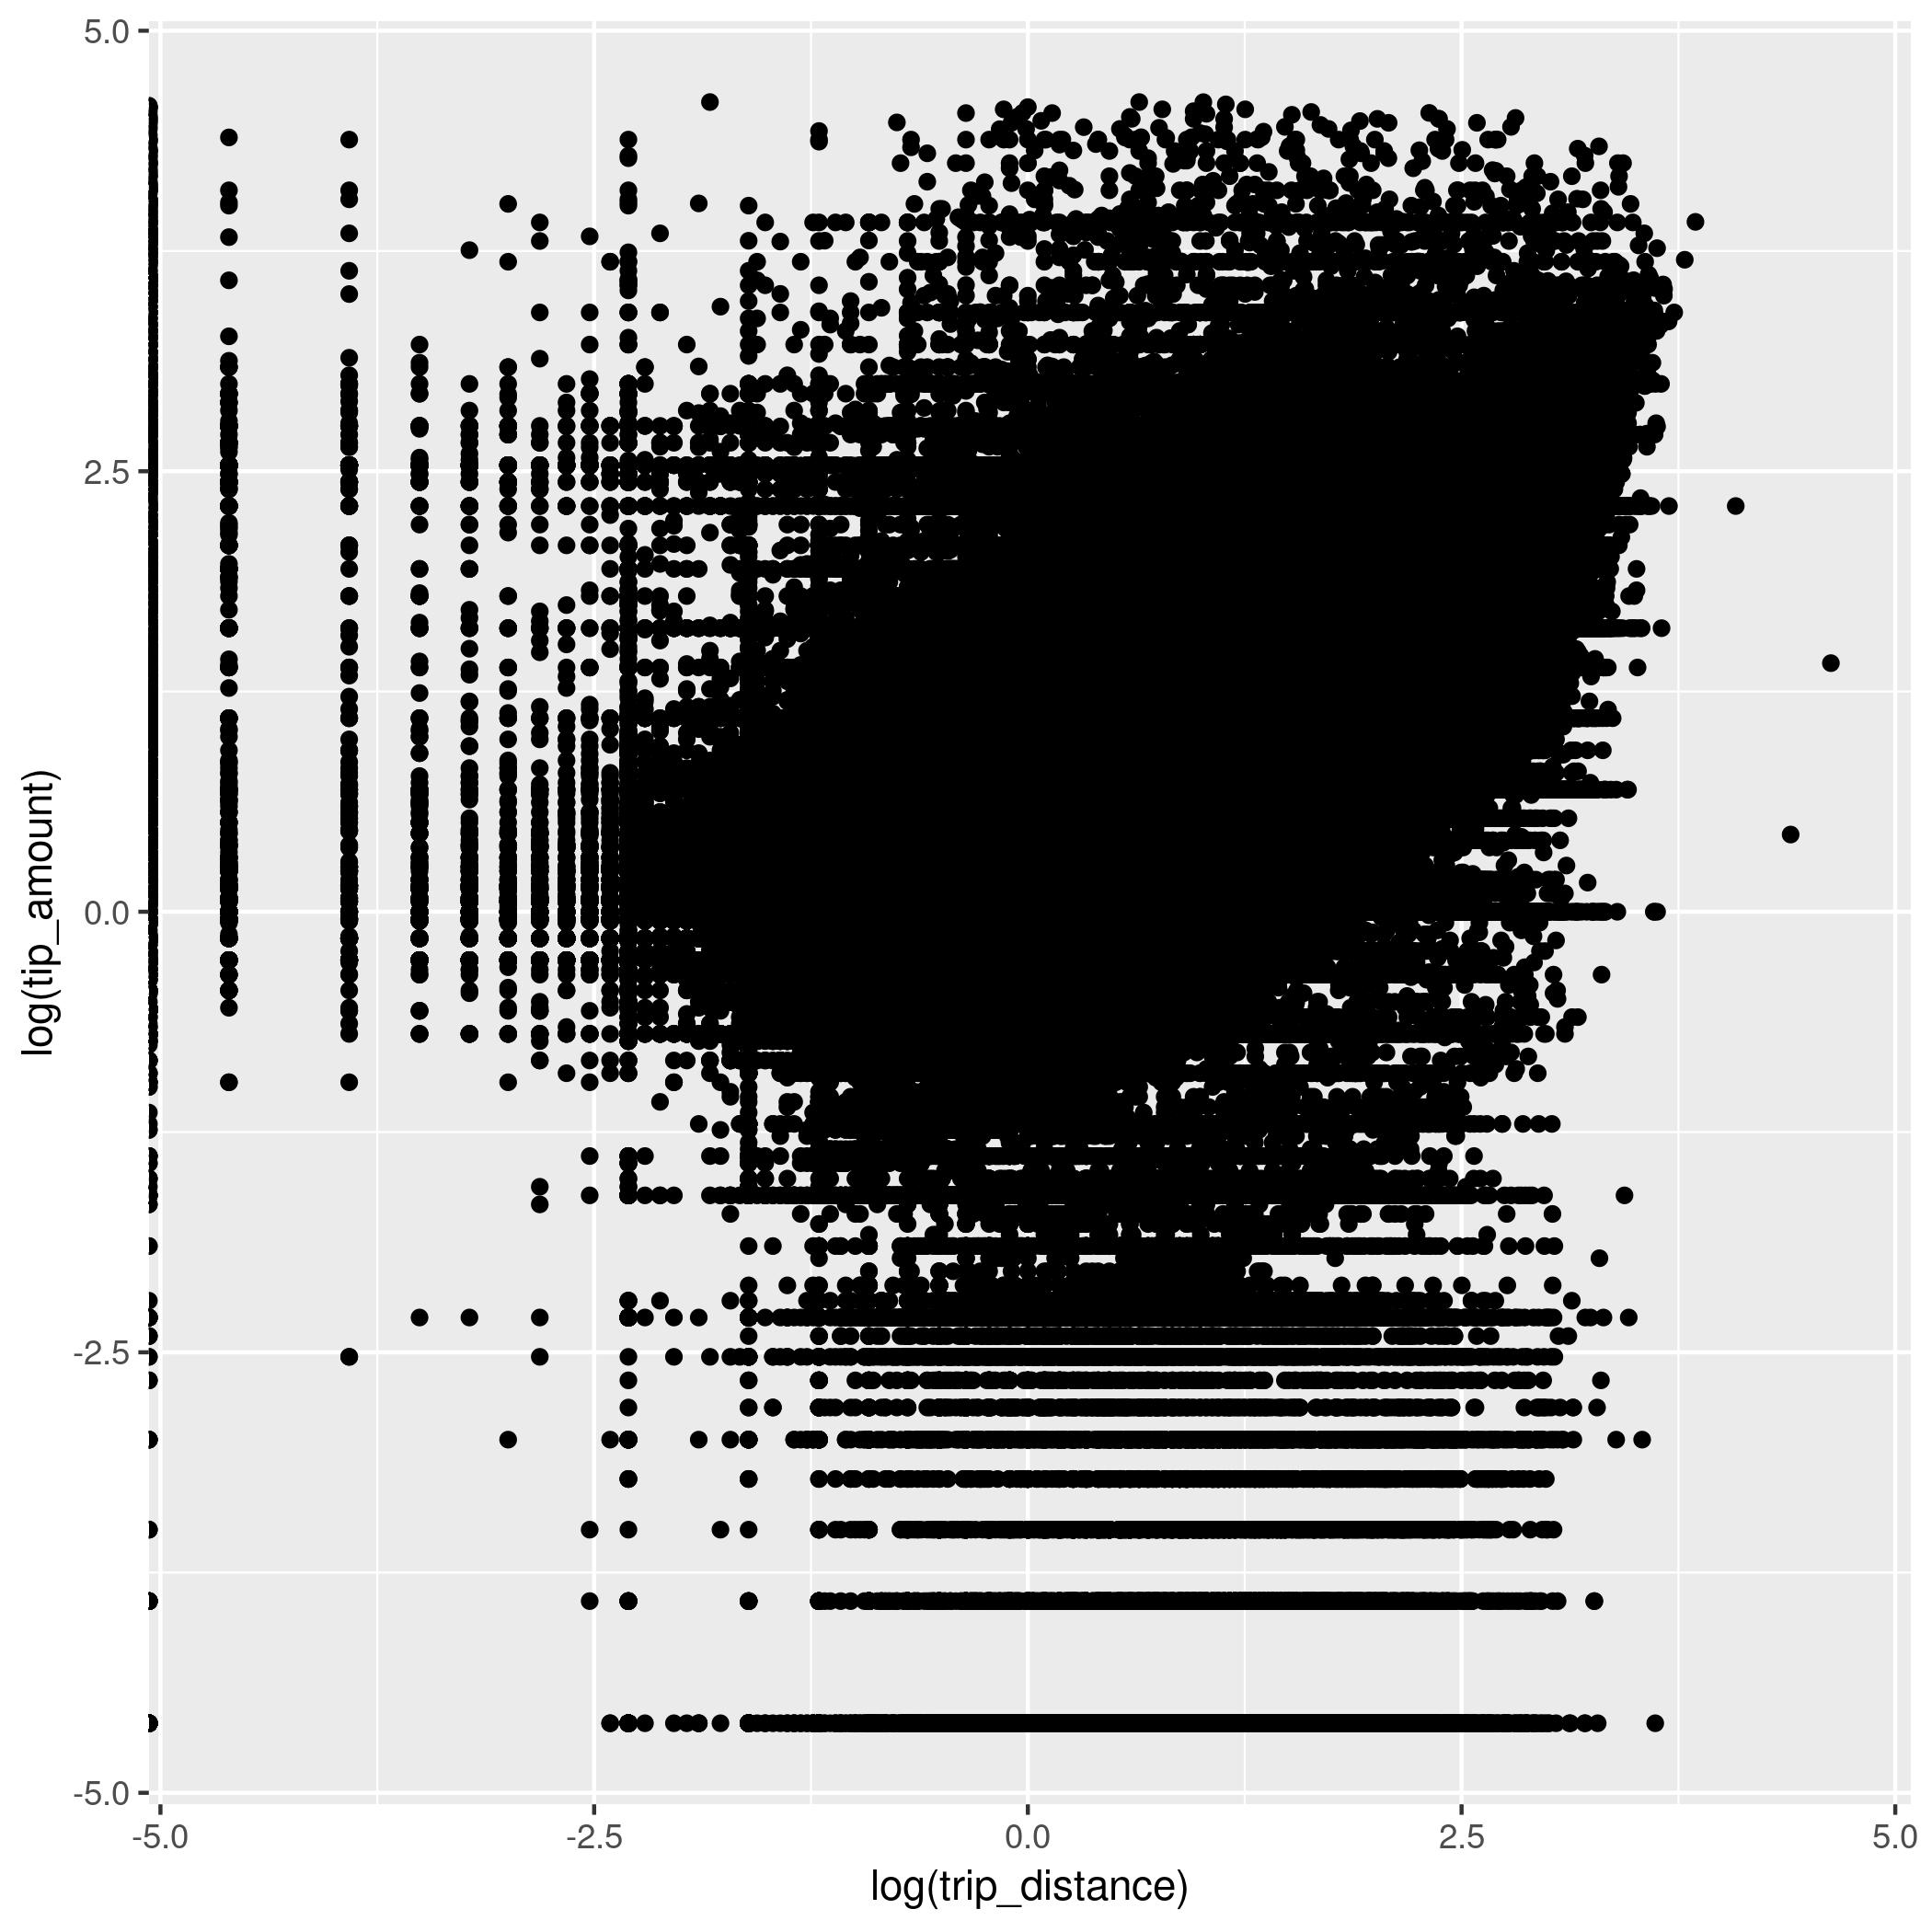
\includegraphics[width=.9\linewidth]{./plots/distanceTipPlot.jpg}
\caption{\label{fig:org392ec20}
Log-tip vs log-distance scatterplot}
\end{figure}

Next two plots look at the \emph{tolls\_amount} variable. Most rides did not
involve a toll, but in the following scatterplot, it is noticeable
that there is some positive correlation when tolls were paid.
\begin{figure}[htbp]
\centering
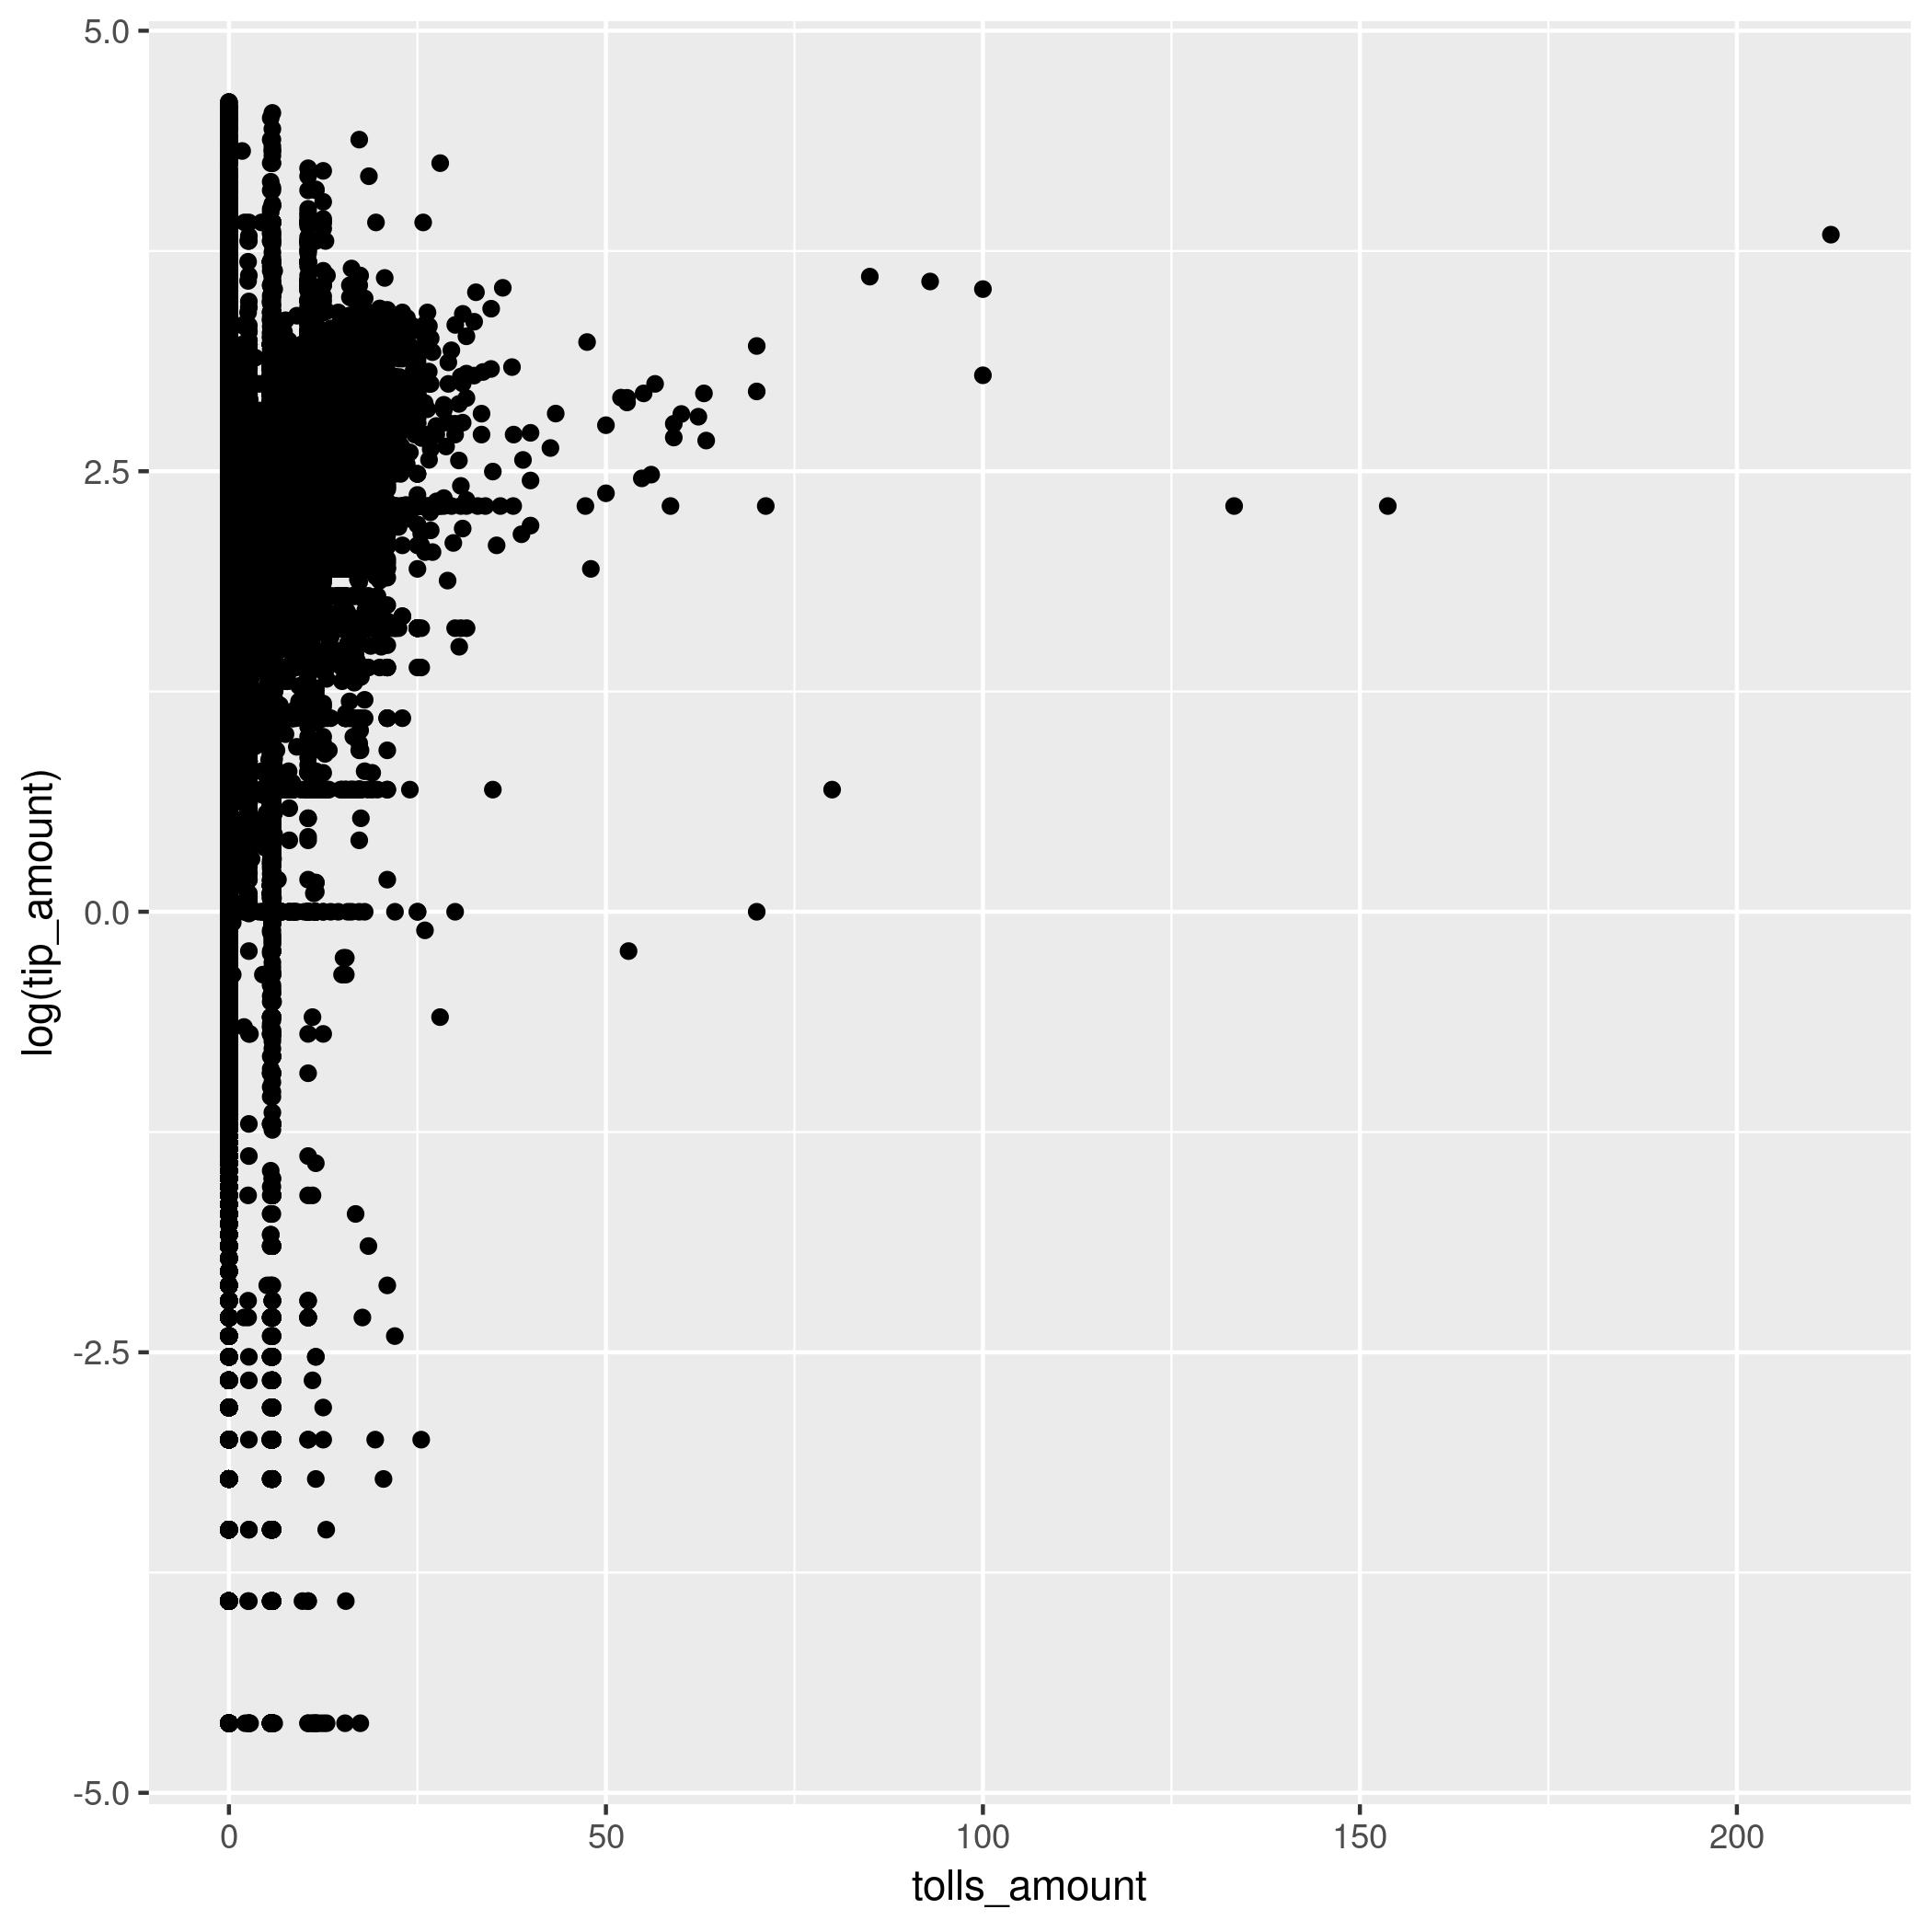
\includegraphics[width=.9\linewidth]{./plots/tollsTipPlot.jpg}
\caption{\label{fig:orgc806998}
Log-tip vs tolls\_amount scatterplot}
\end{figure}

As such, a more sensible variable to include in a model would be a dummy
indicating wheather a toll was paid. Next plot displays there is a
noticeable difference in tip's distribution when a toll is paid.
\begin{figure}[htbp]
\centering
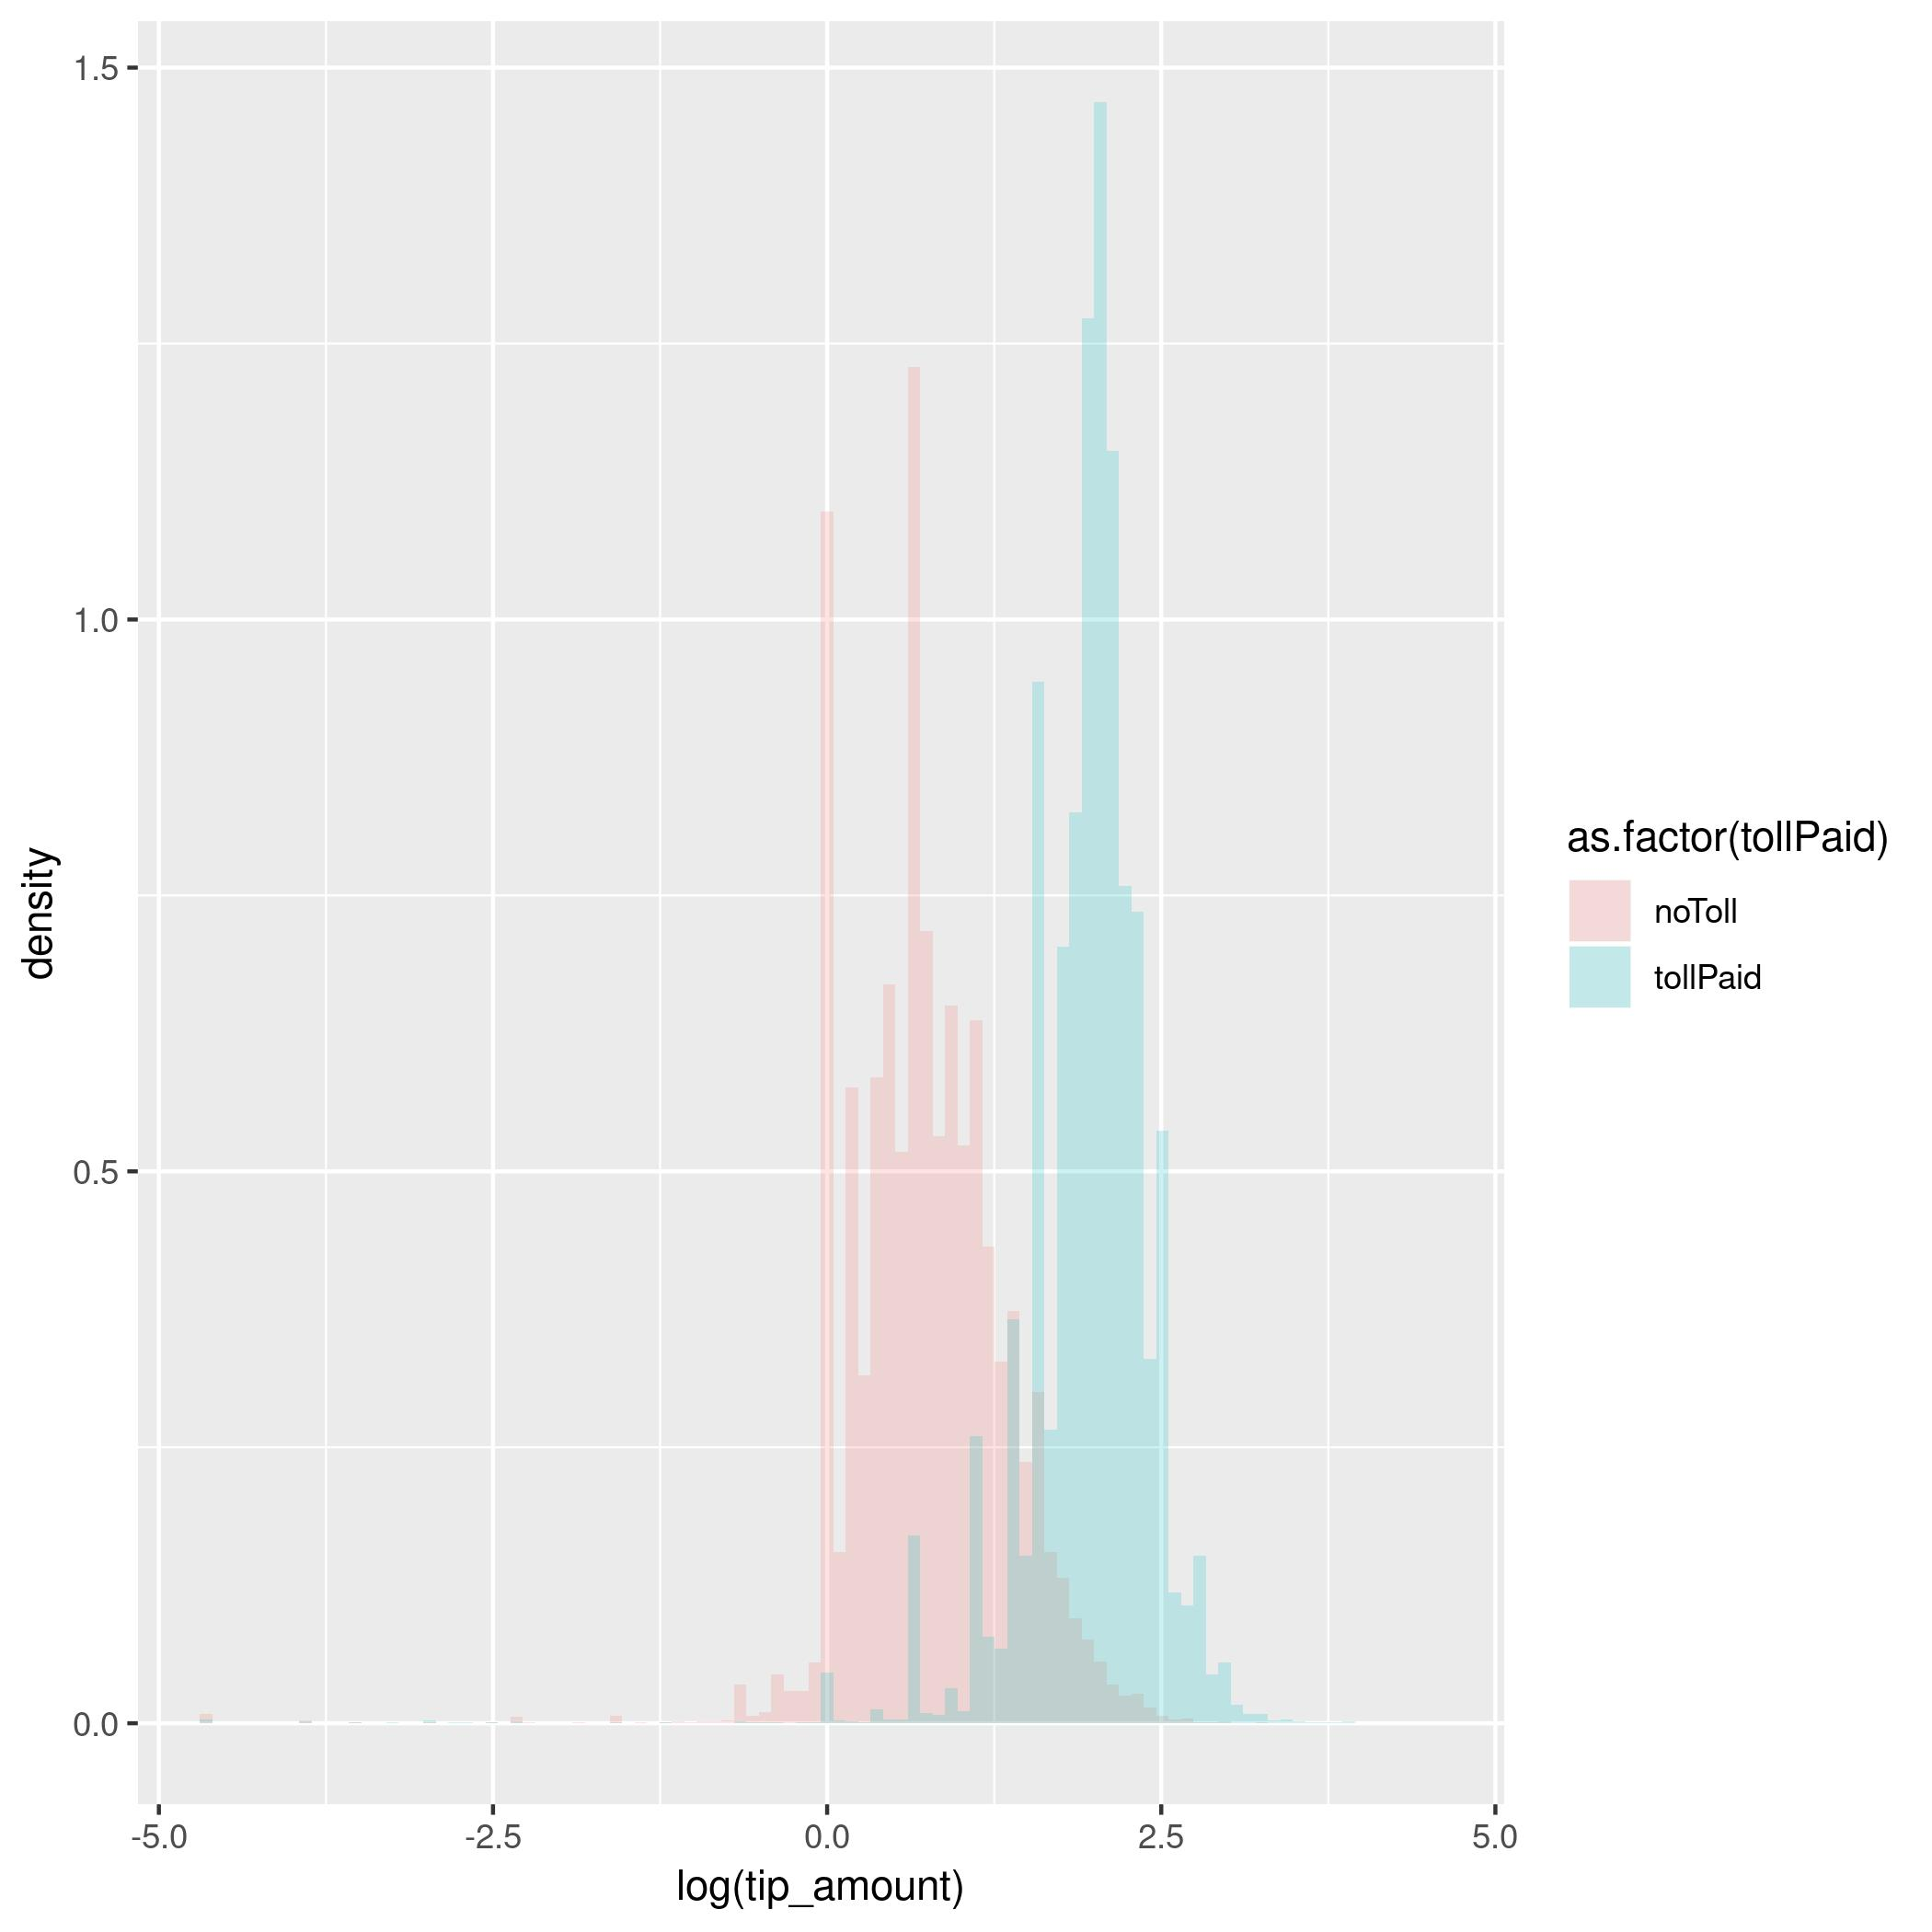
\includegraphics[width=.9\linewidth]{./plots/tollsTipDensityHist.jpg}
\caption{\label{fig:org7e6f626}
Log-tip density histogram by wheather a toll was paid}
\end{figure}

Next two plots help understand tip's relation with \emph{rideTime}.
First we look at the log-rideTime histogram.
\begin{figure}[htbp]
\centering
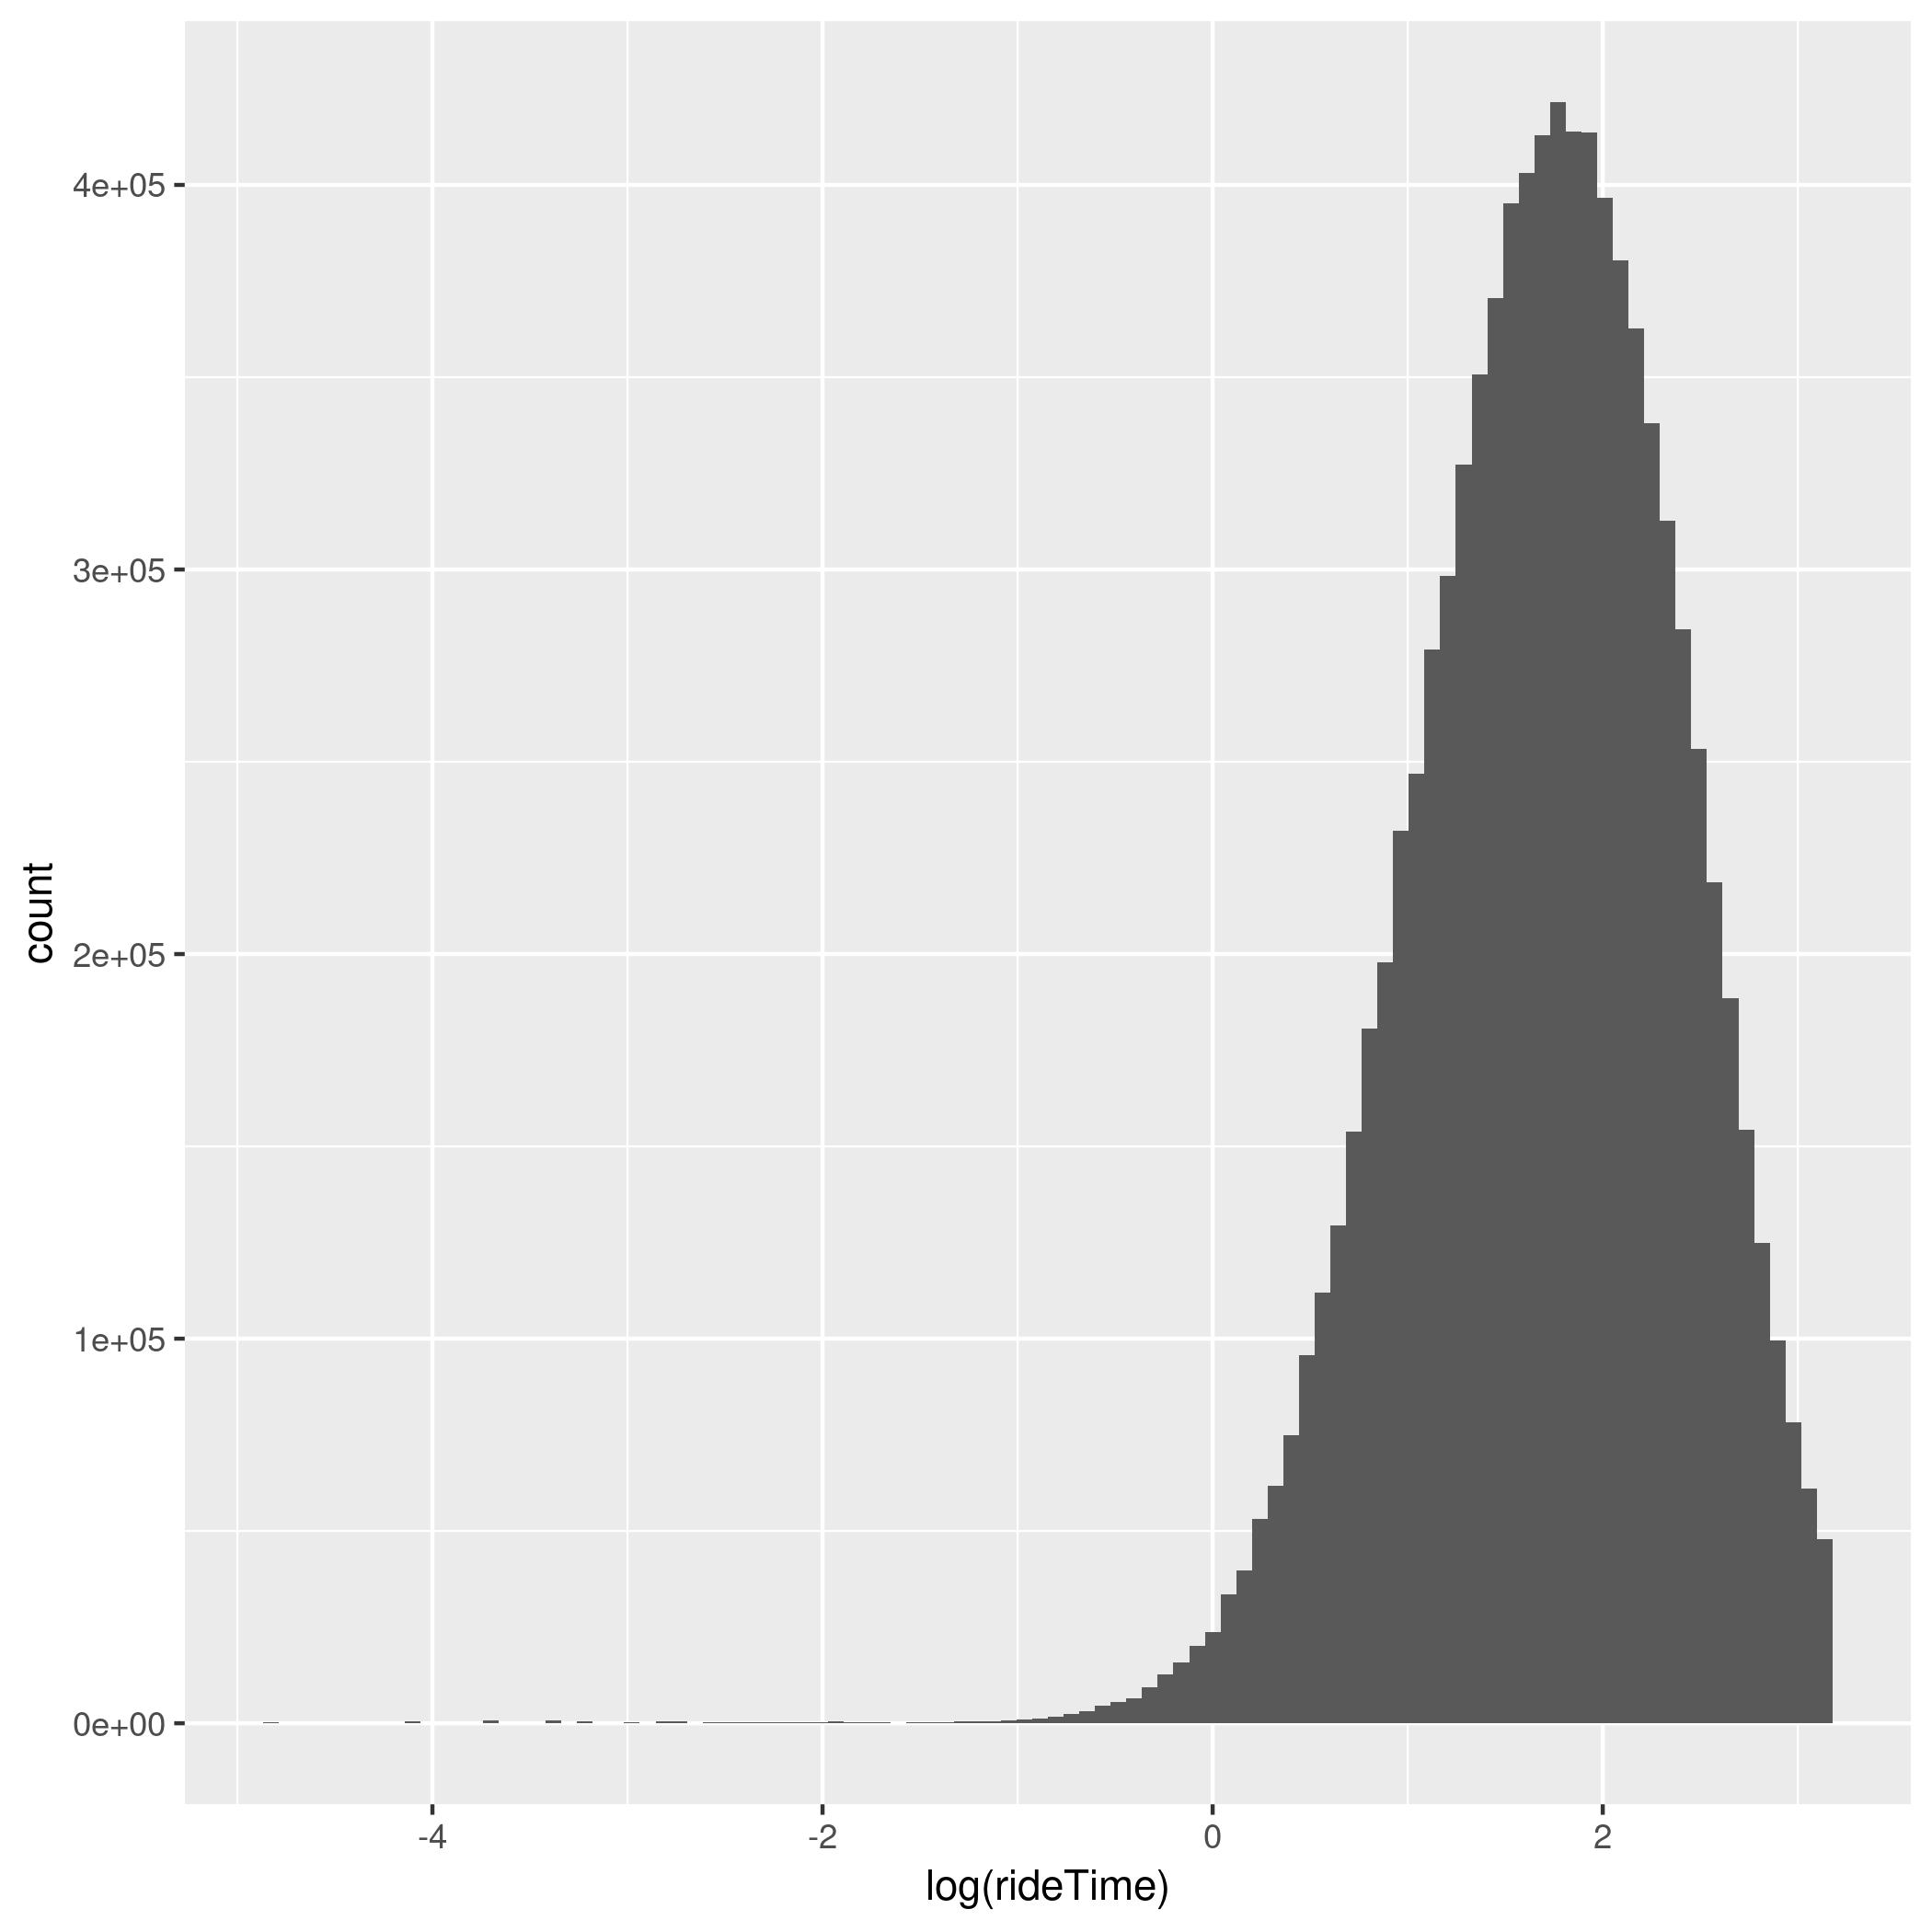
\includegraphics[width=.9\linewidth]{./plots/rideTimeHist.jpg}
\caption{\label{fig:org2bec3ee}
Log-tip ride time histogram}
\end{figure}

Finally we look at tip's correlation with the former variable, again,
strong and positive.
\begin{figure}[htbp]
\centering
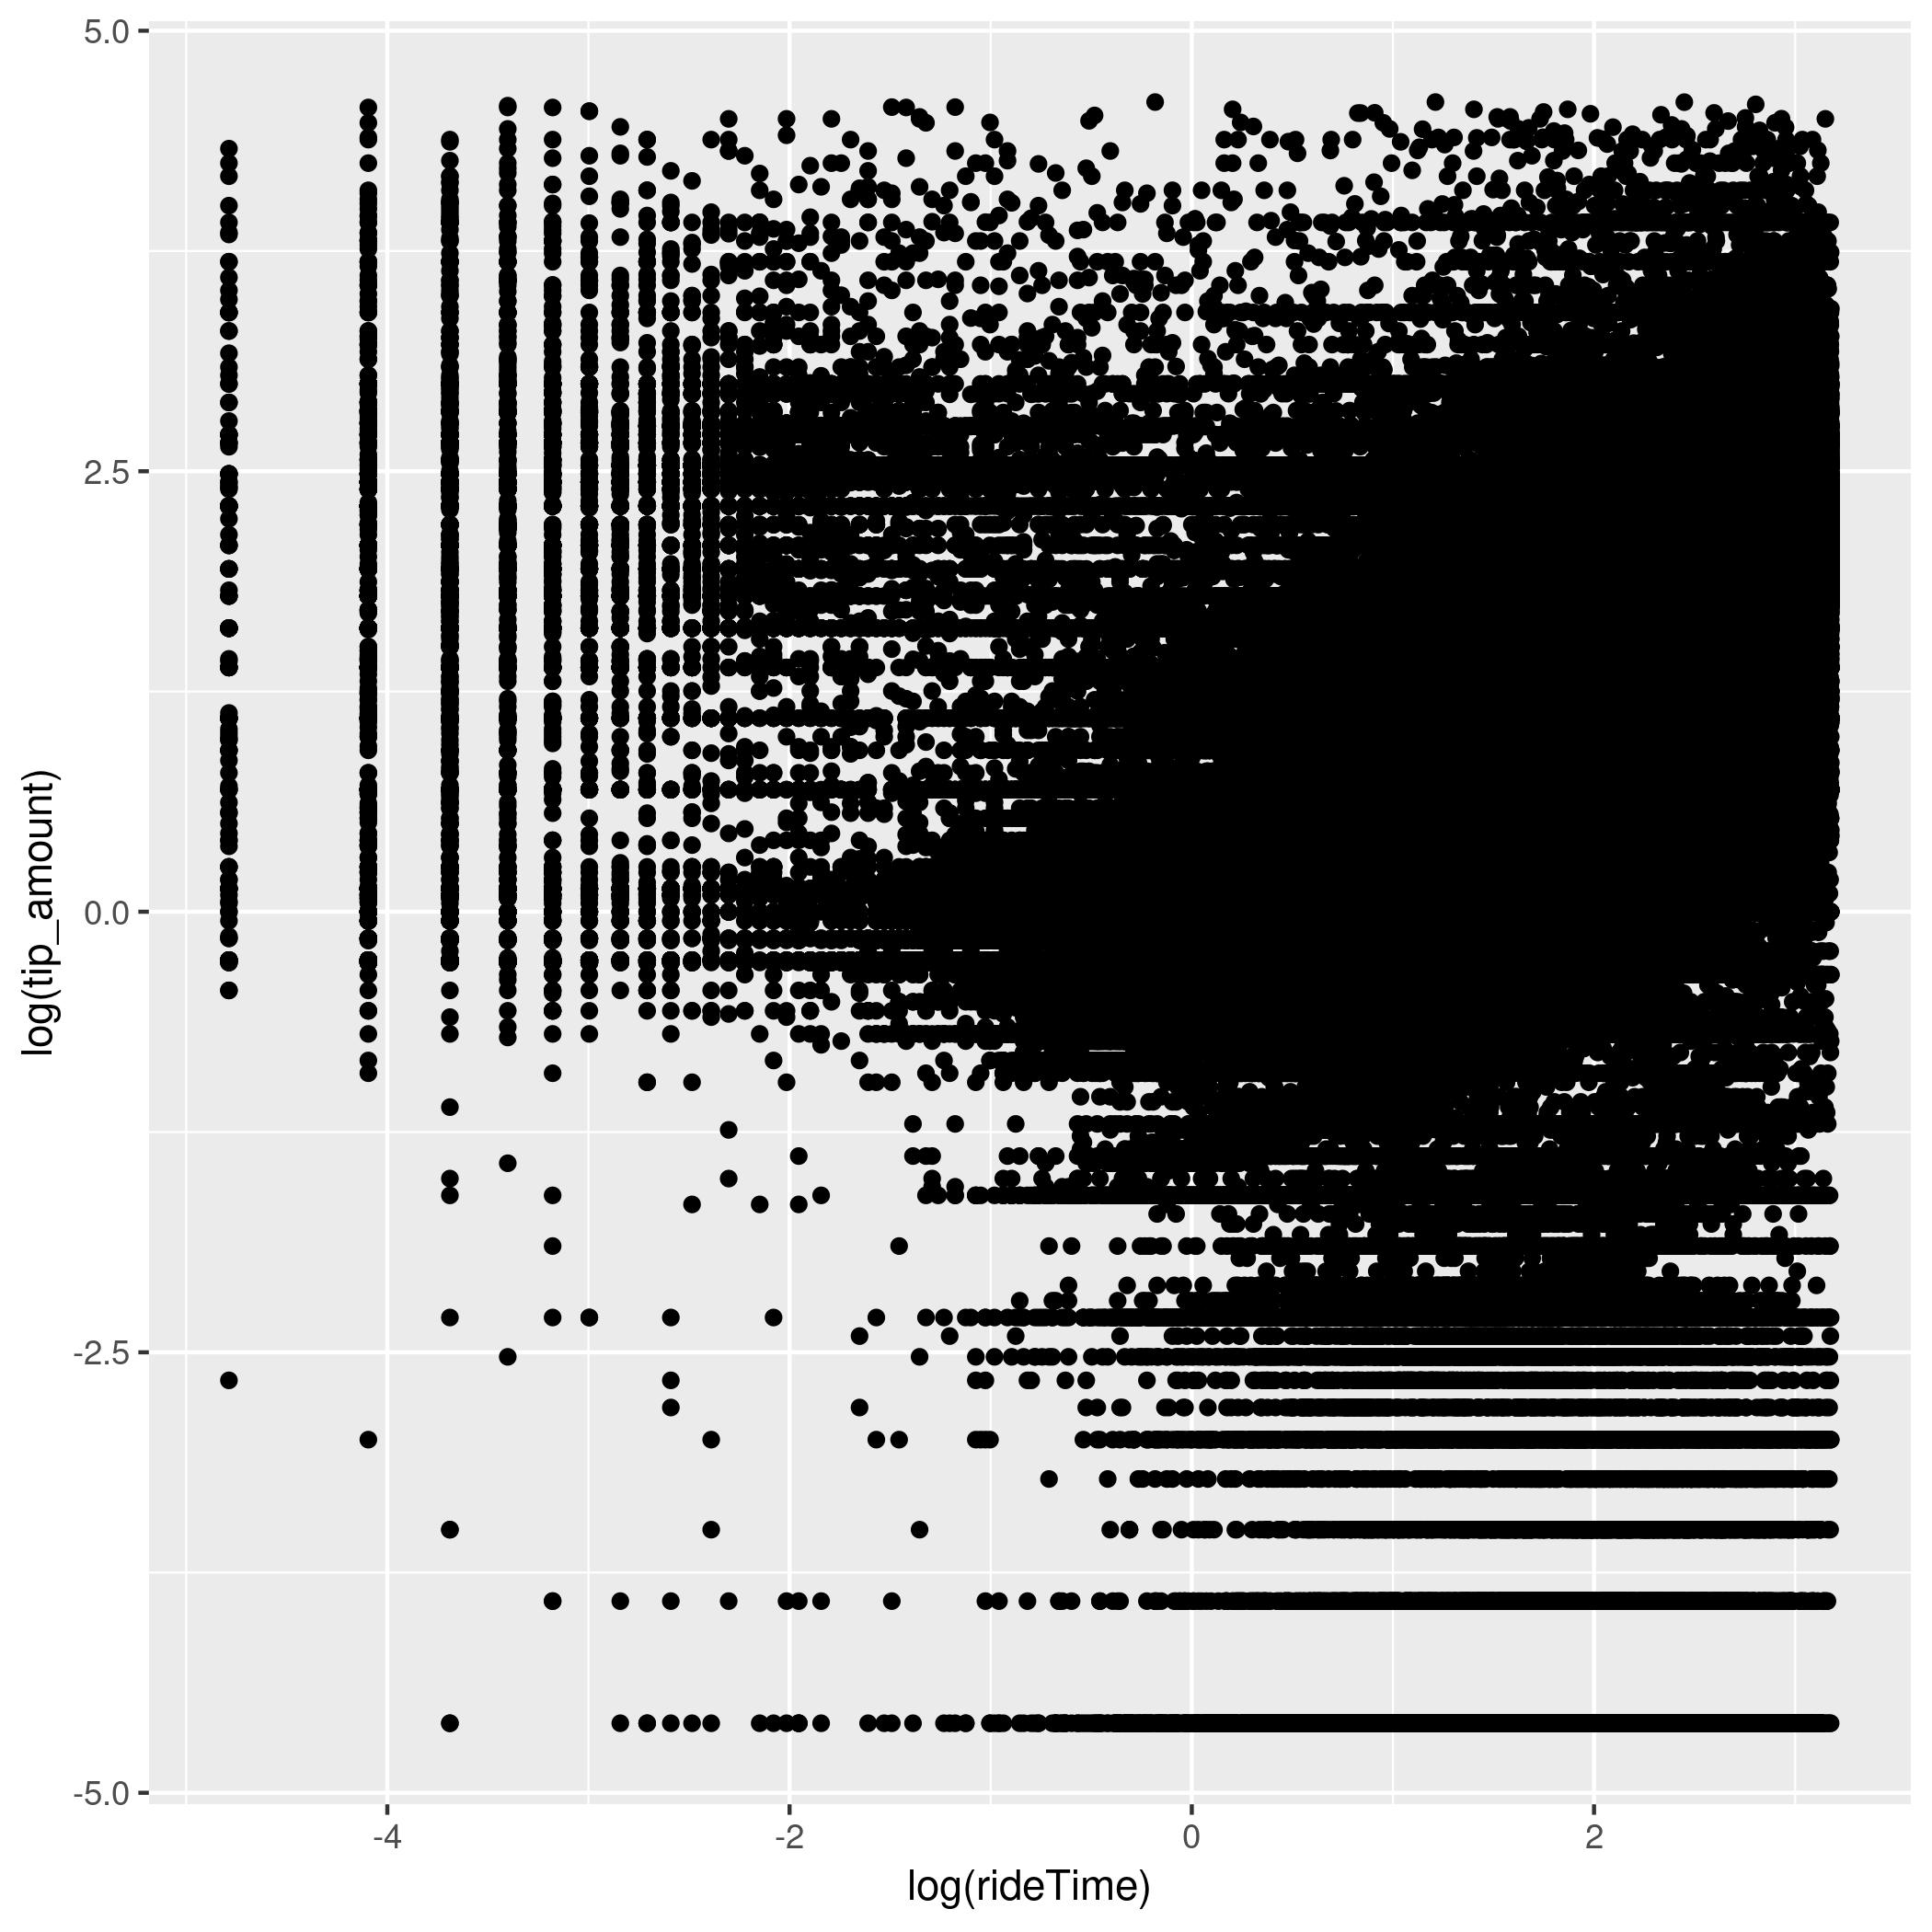
\includegraphics[width=.9\linewidth]{./plots/rideTipPlot.jpg}
\caption{\label{fig:org3e96d2d}
Log-tip vs log-ride-time scatterplot}
\end{figure}


\subsection{spatial visualizations}
\label{sec:orgb8b93c5}

Finally, we are going to take a look at the spatial distributions of the data.

The next two plots showcase the number of trips by pick up and drop off zones.
Other than some key spots, the number of trips, seems to be evenly distriubted
across the map.

\begin{verbatim}
library("tidyverse")
library("ggplot2")
library("ggmap")
library("rgdal")
## library("maps")
## library("maptools")

plotsFolder <- "plots"
shapeFilesFolder <- "shapeFiles"

data <- readRDS("taxiDataFeatures.rds") %>%
    filter(tip_amount < 100) %>%
    filter(tip_amount > 0) %>%
    select(tip_amount, PULocationID) %>%
    rename(LocationID = PULocationID)

data <- data %>% group_by(LocationID) %>%
    summarise(numRides = n())

taxiArea <- readOGR(shapeFilesFolder)
taxiArea@data <- data %>% right_join(taxiArea@data, "LocationID")
taxiArea@data %>% summary
taxiAreaDf <- fortify(taxiArea)

taxiAreaDf <- taxiAreaDf %>%
    inner_join(taxiArea@data %>%
               rename(id = LocationID) %>%
               mutate(id = id %>% as.character), "id") %>%
    drop_na


pickupTipMap <- ggplot(taxiAreaDf, aes(long, lat, group = group, fill = taxiAreaDf$numRides)) +
    geom_polygon() + geom_path(alpha = 0.3) + coord_equal() + theme_classic() +
    labs(fill = "Trip count")
ggsave(paste(plotsFolder, "pickupTripsMap.jpg", sep = "/"), pickupTipMap)
\end{verbatim}

\begin{figure}[htbp]
\centering
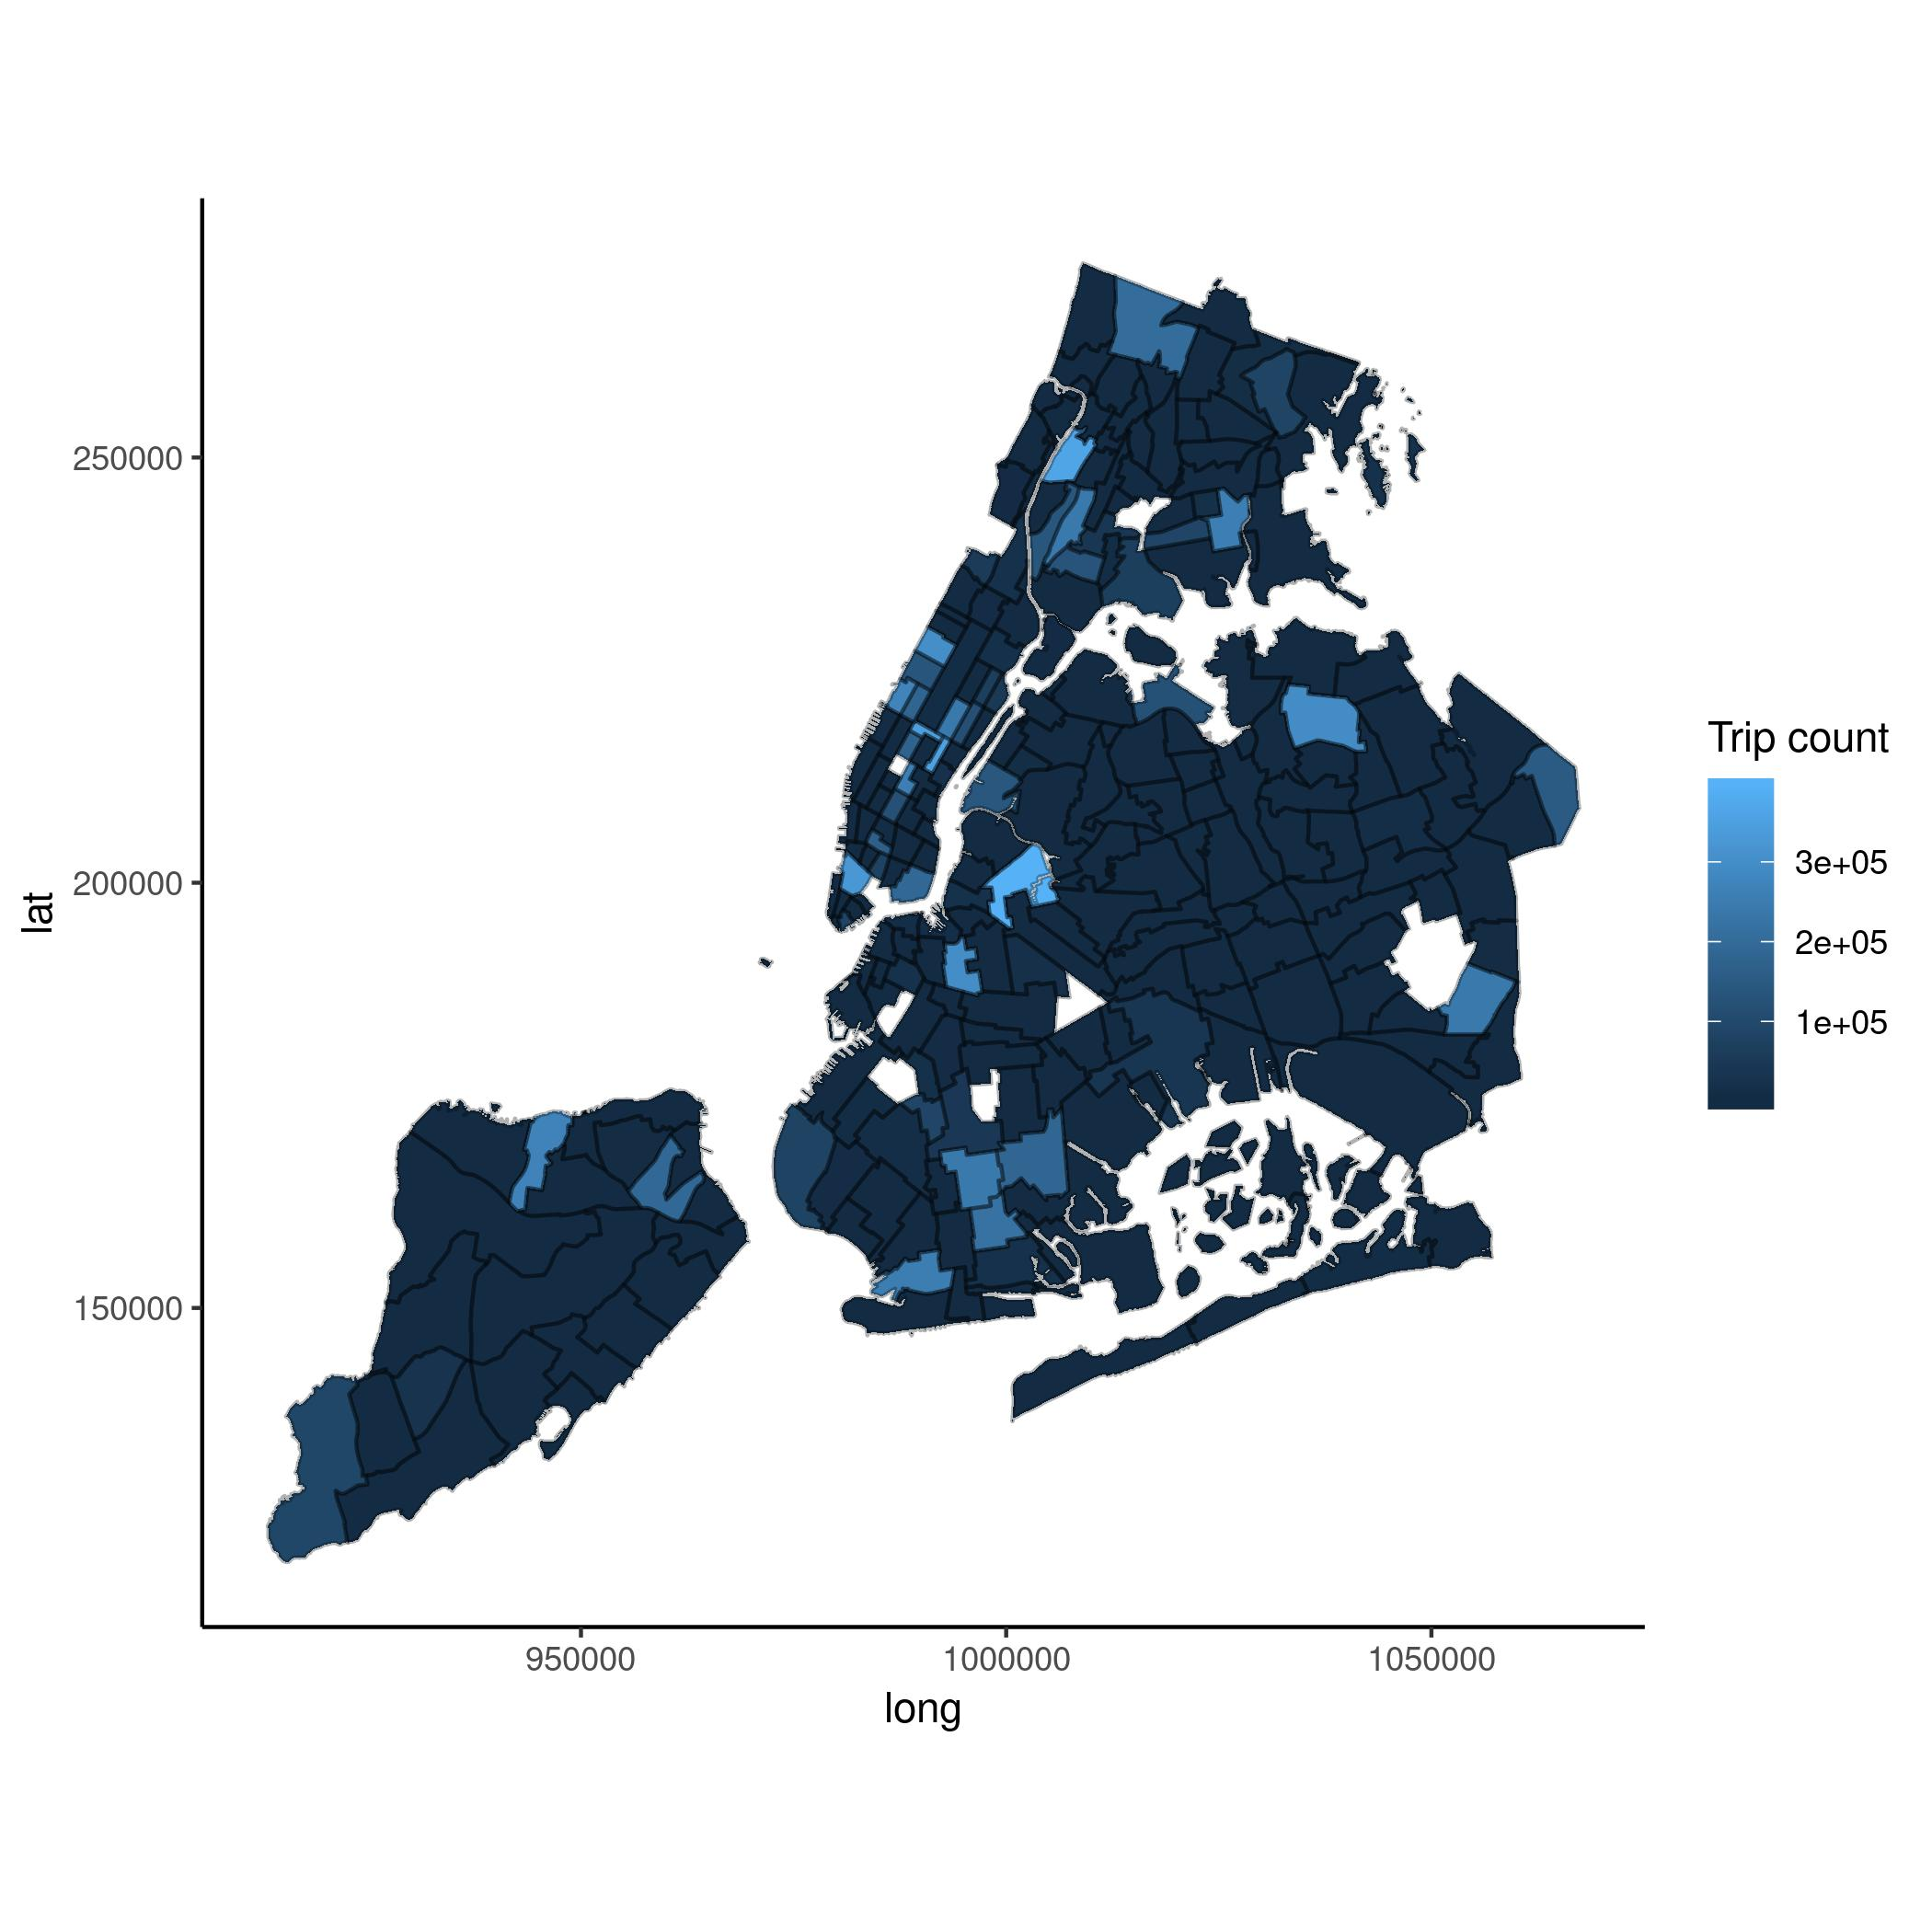
\includegraphics[width=.9\linewidth]{./plots/pickupTripsMap.jpg}
\caption{\label{fig:orgee0c997}
Trip count by taxi pickup zone}
\end{figure}



\begin{verbatim}
library("tidyverse")
library("ggplot2")
library("ggmap")
library("rgdal")
## library("maps")
## library("maptools")

plotsFolder <- "plots"
shapeFilesFolder <- "shapeFiles"

data <- readRDS("taxiDataFeatures.rds") %>%
    filter(tip_amount < 100) %>%
    filter(tip_amount > 0) %>%
    select(tip_amount, DOLocationID) %>%
    rename(LocationID = DOLocationID)

data <- data %>% group_by(LocationID) %>%
    summarise(numRides = n())

taxiArea <- readOGR(shapeFilesFolder)
taxiArea@data <- data %>% right_join(taxiArea@data, "LocationID")
taxiArea@data %>% summary
taxiAreaDf <- fortify(taxiArea)

taxiAreaDf <- taxiAreaDf %>%
    inner_join(taxiArea@data %>%
               rename(id = LocationID) %>%
               mutate(id = id %>% as.character), "id") %>%
    drop_na

destinationTipMap <- ggplot(taxiAreaDf, aes(long, lat, group = group, fill = taxiAreaDf$numRideso)) +
    geom_polygon() + geom_path(alpha = 0.3) + coord_equal() + theme_classic() +
    labs(fill = "Trip count")
ggsave(paste(plotsFolder, "destinationTripsMap.jpg", sep = "/"), destinationTipMap)
\end{verbatim}

\begin{figure}[htbp]
\centering
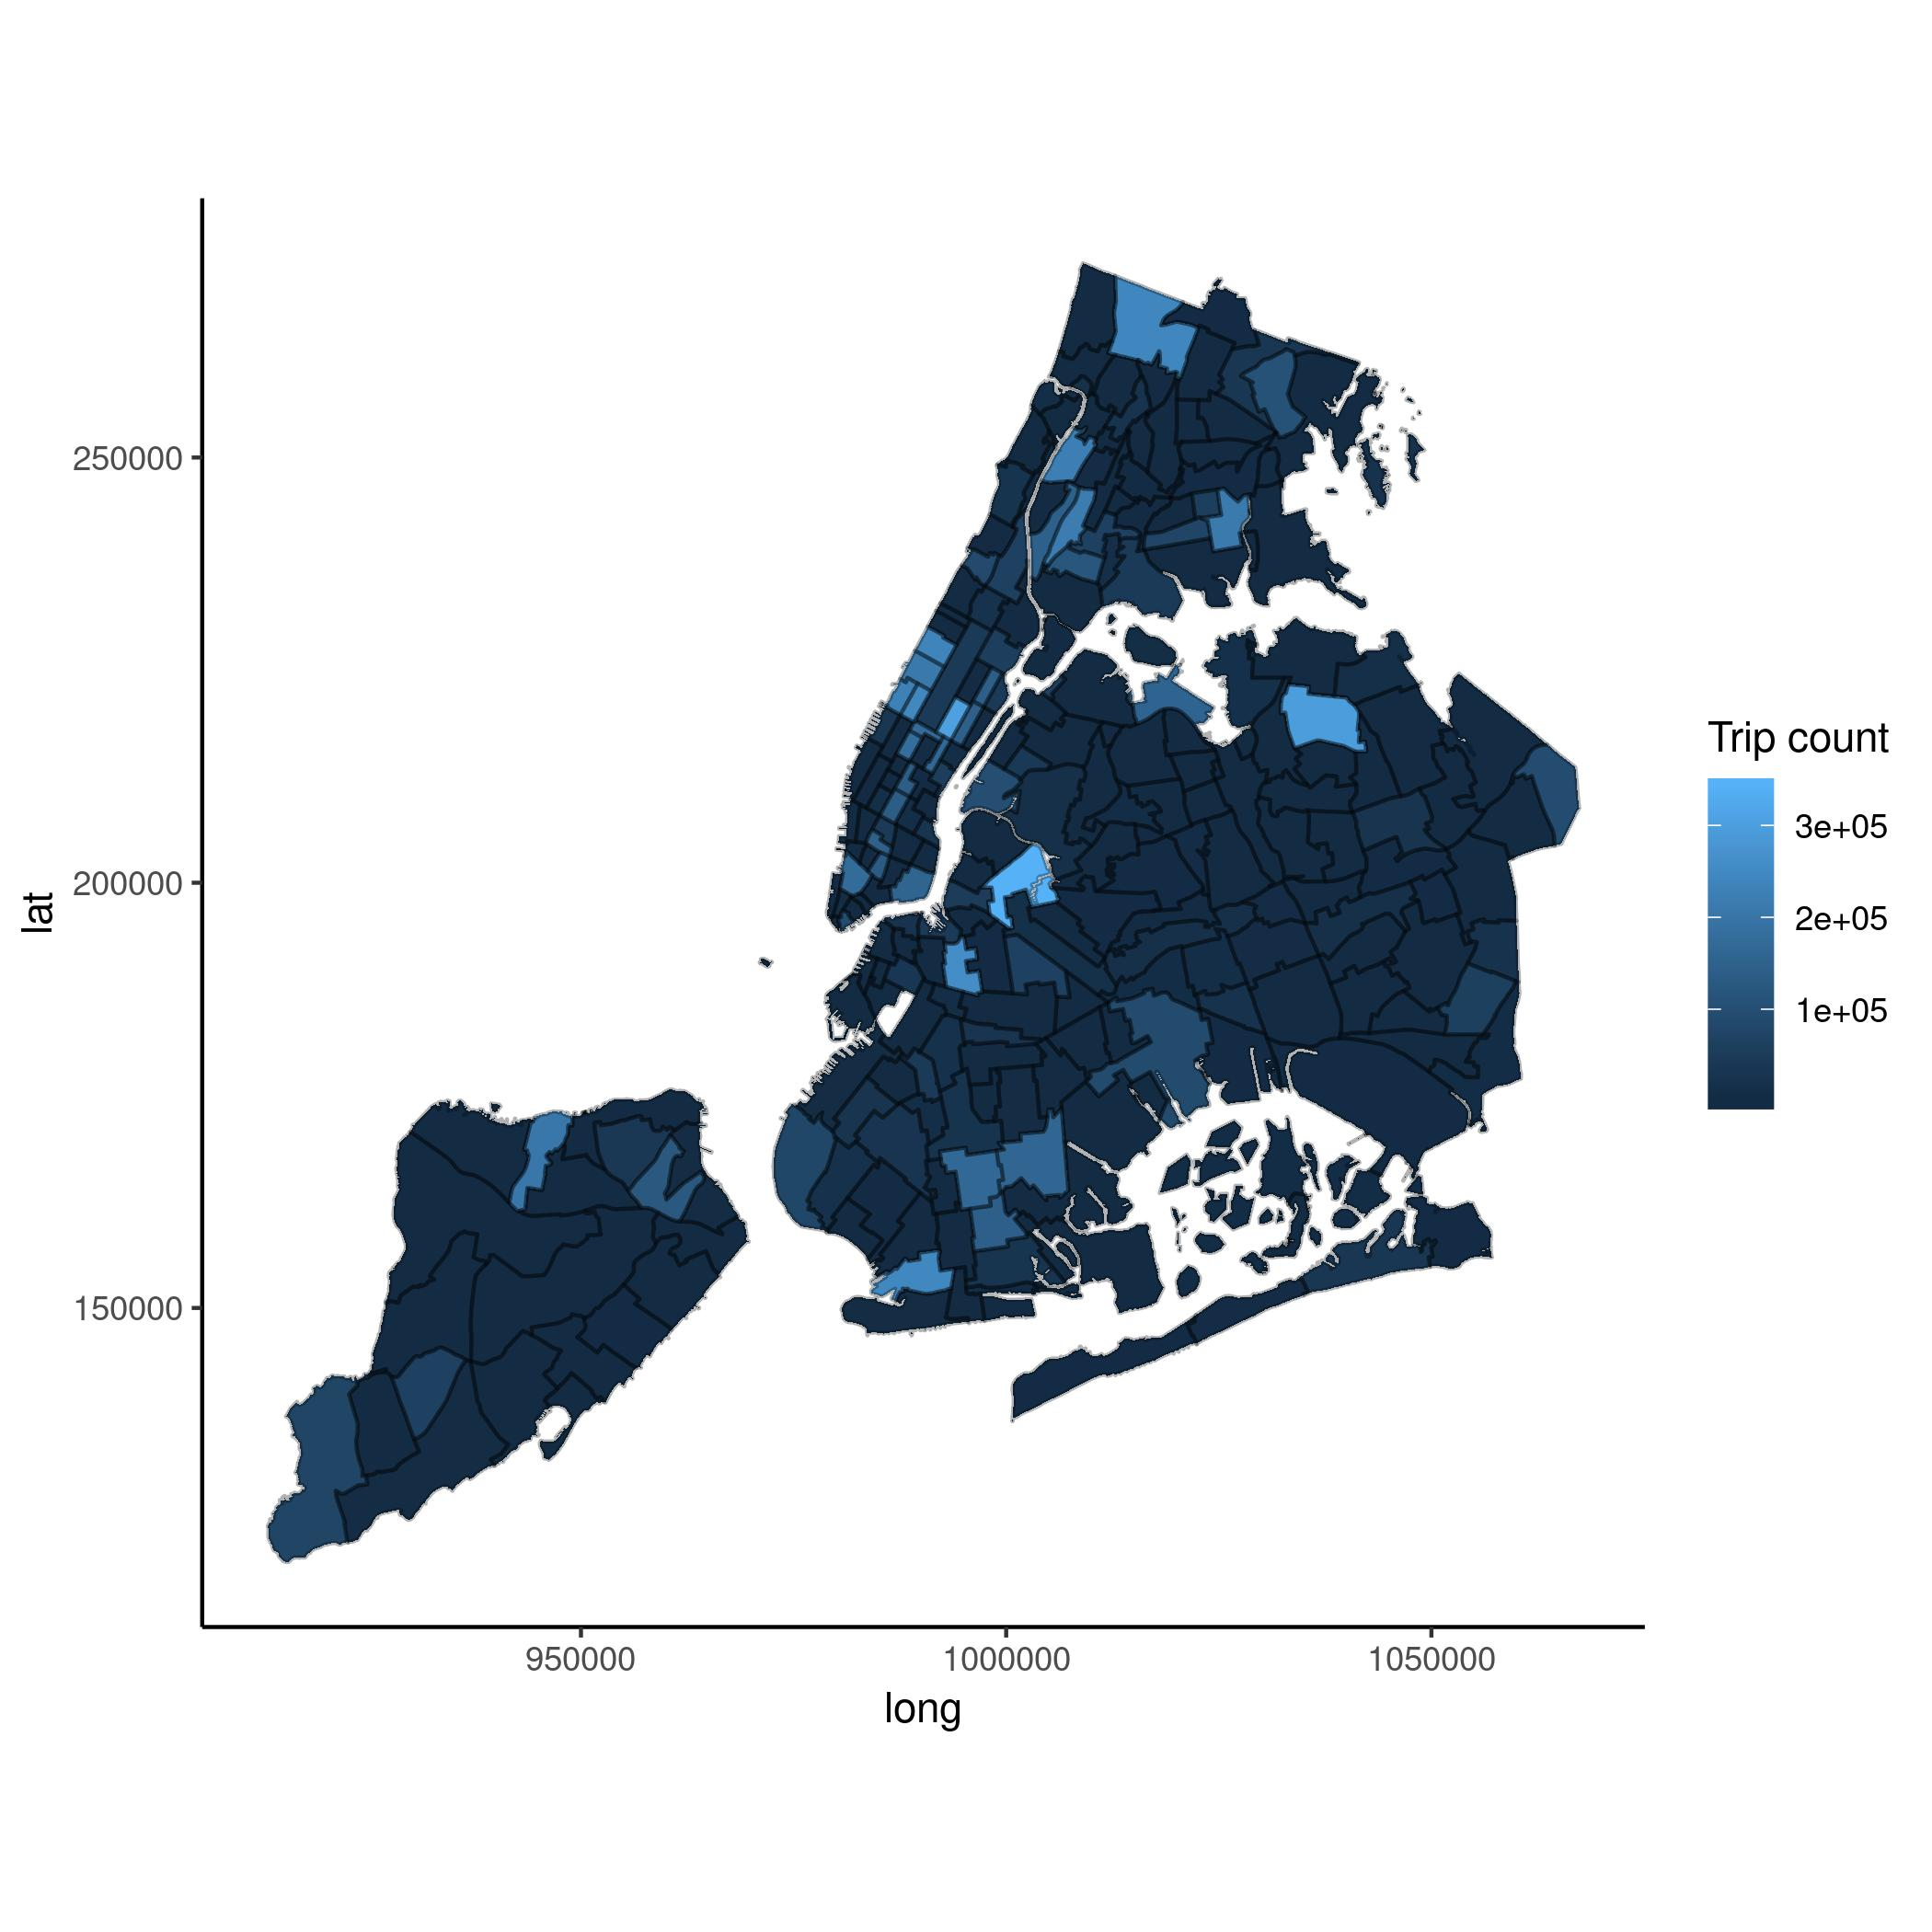
\includegraphics[width=.9\linewidth]{./plots/destinationTripsMap.jpg}
\caption{\label{fig:org8aa1d26}
Trip count by taxi dropoff zone}
\end{figure}

\begin{verbatim}
library("tidyverse")
library("ggplot2")
library("ggmap")
library("rgdal")
## library("maps")
## library("maptools")

plotsFolder <- "plots"
shapeFilesFolder <- "shapeFiles"

data <- readRDS("taxiDataFeatures.rds") %>%
    filter(tip_amount < 100) %>%
    filter(tip_amount > 0) %>%
    select(tip_amount, DOLocationID) %>%
    rename(LocationID = DOLocationID)
?group_by
data <- data %>% group_by(LocationID) %>%
    summarise(tip_amount = median(tip_amount))

taxiArea <- readOGR(shapeFilesFolder)
taxiArea@data <- data %>% right_join(taxiArea@data, "LocationID")
taxiArea@data %>% summary
taxiAreaDf <- fortify(taxiArea)

taxiAreaDf <- taxiAreaDf %>%
    inner_join(taxiArea@data %>%
               rename(id = LocationID) %>%
               mutate(id = id %>% as.character), "id") %>%
    drop_na

taxiAreaDf$tip_amount %>% length

destinationTipMap <- ggplot(taxiAreaDf, aes(long, lat, group = group, fill = taxiAreaDf$tip_amount)) +
    geom_polygon() + geom_path(alpha = 0.3) + coord_equal() + theme_classic() +
    labs(fill = "Median tip")
ggsave(paste(plotsFolder, "destinationTipMap.jpg", sep = "/"), destinationTipMap)

\end{verbatim}

In the next two plots, the median tip (the median is choosen over the mean
to mitigate the effect of outliers) by pick up and drop off zone. By pick up
zone, the tips seem to be more evenly distributed, while by drop off zone,
there seems to be more difference among taxi zones. Furthermore, by pick up
zone, the median tip is truncated at \$20, as there are some strong outliers,
that would distort the plot and show even less difference between the zones.

With this information, when it comes to modelling, seems like drop off, rather
than pick up, will be more interisting. also, there are some empty regions in the
pick up map.

\begin{figure}[htbp]
\centering
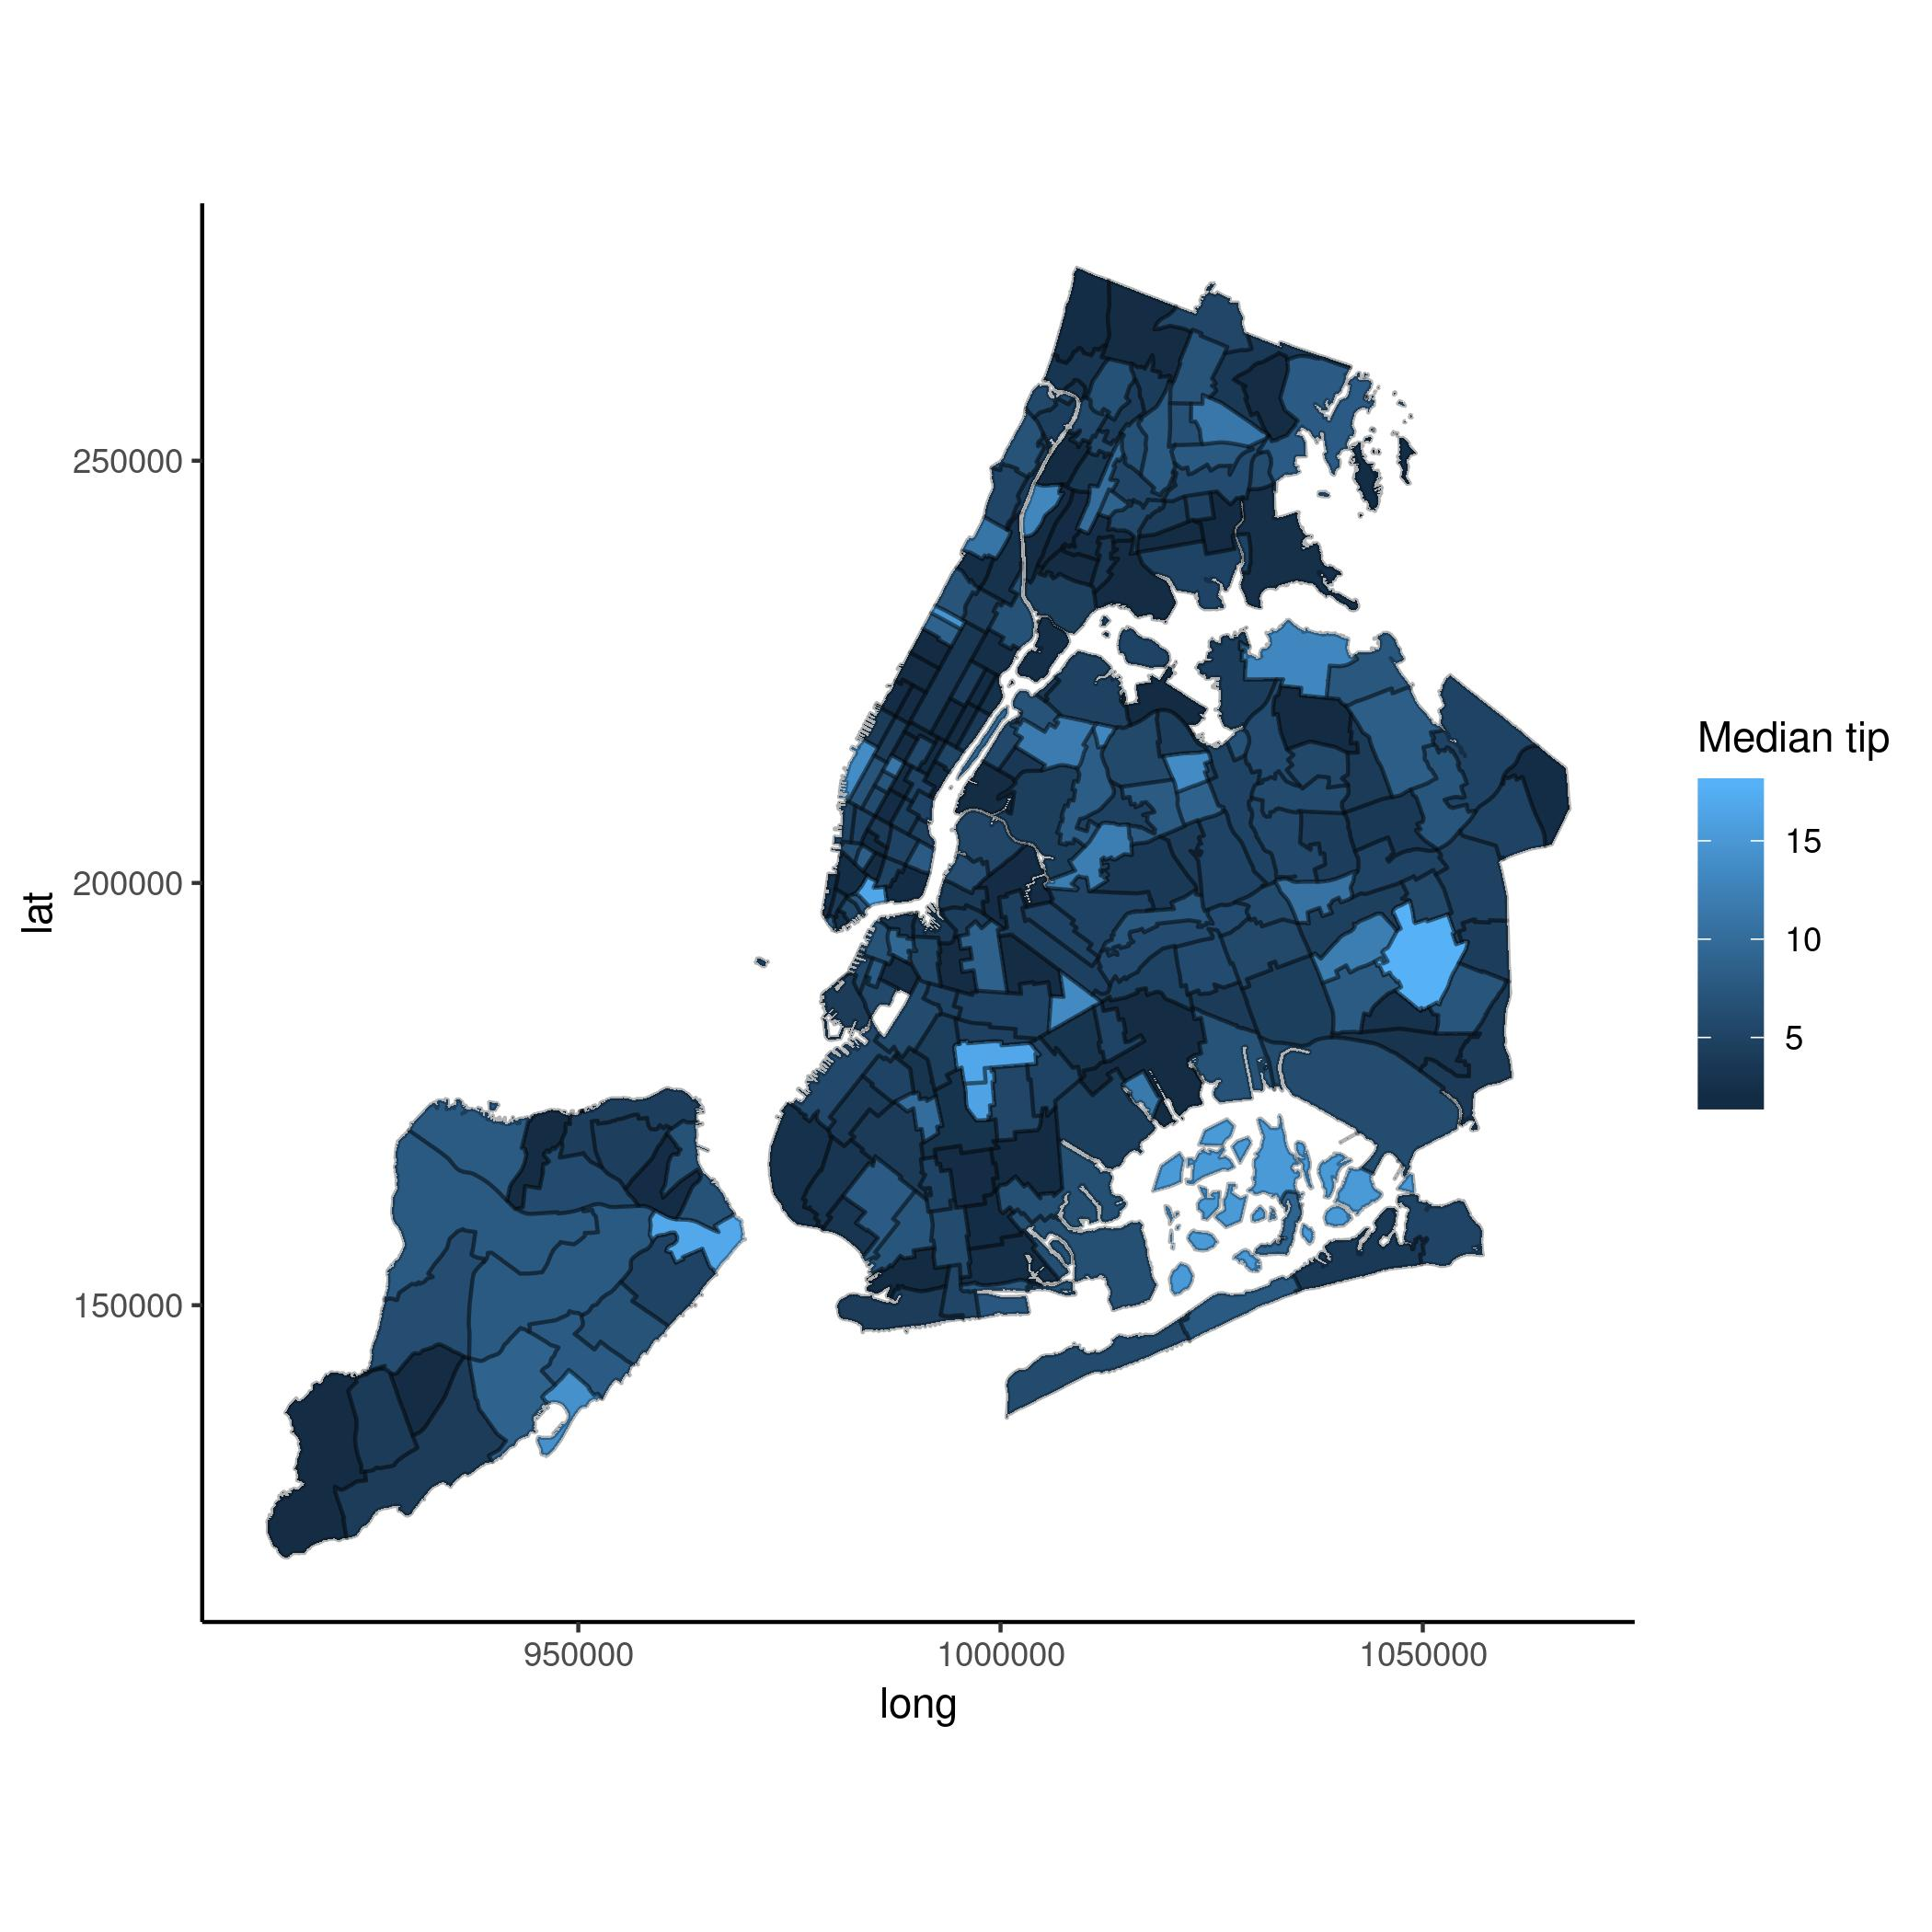
\includegraphics[width=.9\linewidth]{./plots/destinationTipMap.jpg}
\caption{\label{fig:org38fb0c4}
Median tip by taxi dropoff zone}
\end{figure}

\begin{verbatim}
library("tidyverse")
library("ggplot2")
library("ggmap")
library("rgdal")
## library("maps")
## library("maptools")

plotsFolder <- "plots"
shapeFilesFolder <- "shapeFiles"

data <- readRDS("taxiDataFeatures.rds") %>%
    filter(tip_amount < 100) %>%
    filter(tip_amount > 0) %>%
    select(tip_amount, PULocationID) %>%
    rename(LocationID = PULocationID)

data <- data %>% group_by(LocationID) %>%
    summarise(tip_amount = mean(tip_amount))
data$tip_amount[data$tip_amount > 20] <- 20

## taxiArea@data %>% select(LocationID, borough) %>%
##     saveRDS("boroughData.rds")

taxiArea <- readOGR(shapeFilesFolder)
taxiArea@data <- data %>% right_join(taxiArea@data, "LocationID")
taxiArea@data %>% summary
taxiAreaDf <- fortify(taxiArea)

taxiAreaDf <- taxiAreaDf %>%
    inner_join(taxiArea@data %>%
               rename(id = LocationID) %>%
               mutate(id = id %>% as.character), "id") %>%
    drop_na

taxiAreaDf$tip_amount %>% length

pickupTipMap <- ggplot(taxiAreaDf, aes(long, lat, group = group, fill = taxiAreaDf$tip_amount)) +
    geom_polygon() + geom_path(alpha = 0.3) + coord_equal() + theme_classic() +
    labs(fill = "Median tip")
pickupTipMap
ggsave(paste(plotsFolder, "pickupTipMap.jpg", sep = "/"), pickupTipMap)


\end{verbatim}

\begin{figure}[htbp]
\centering
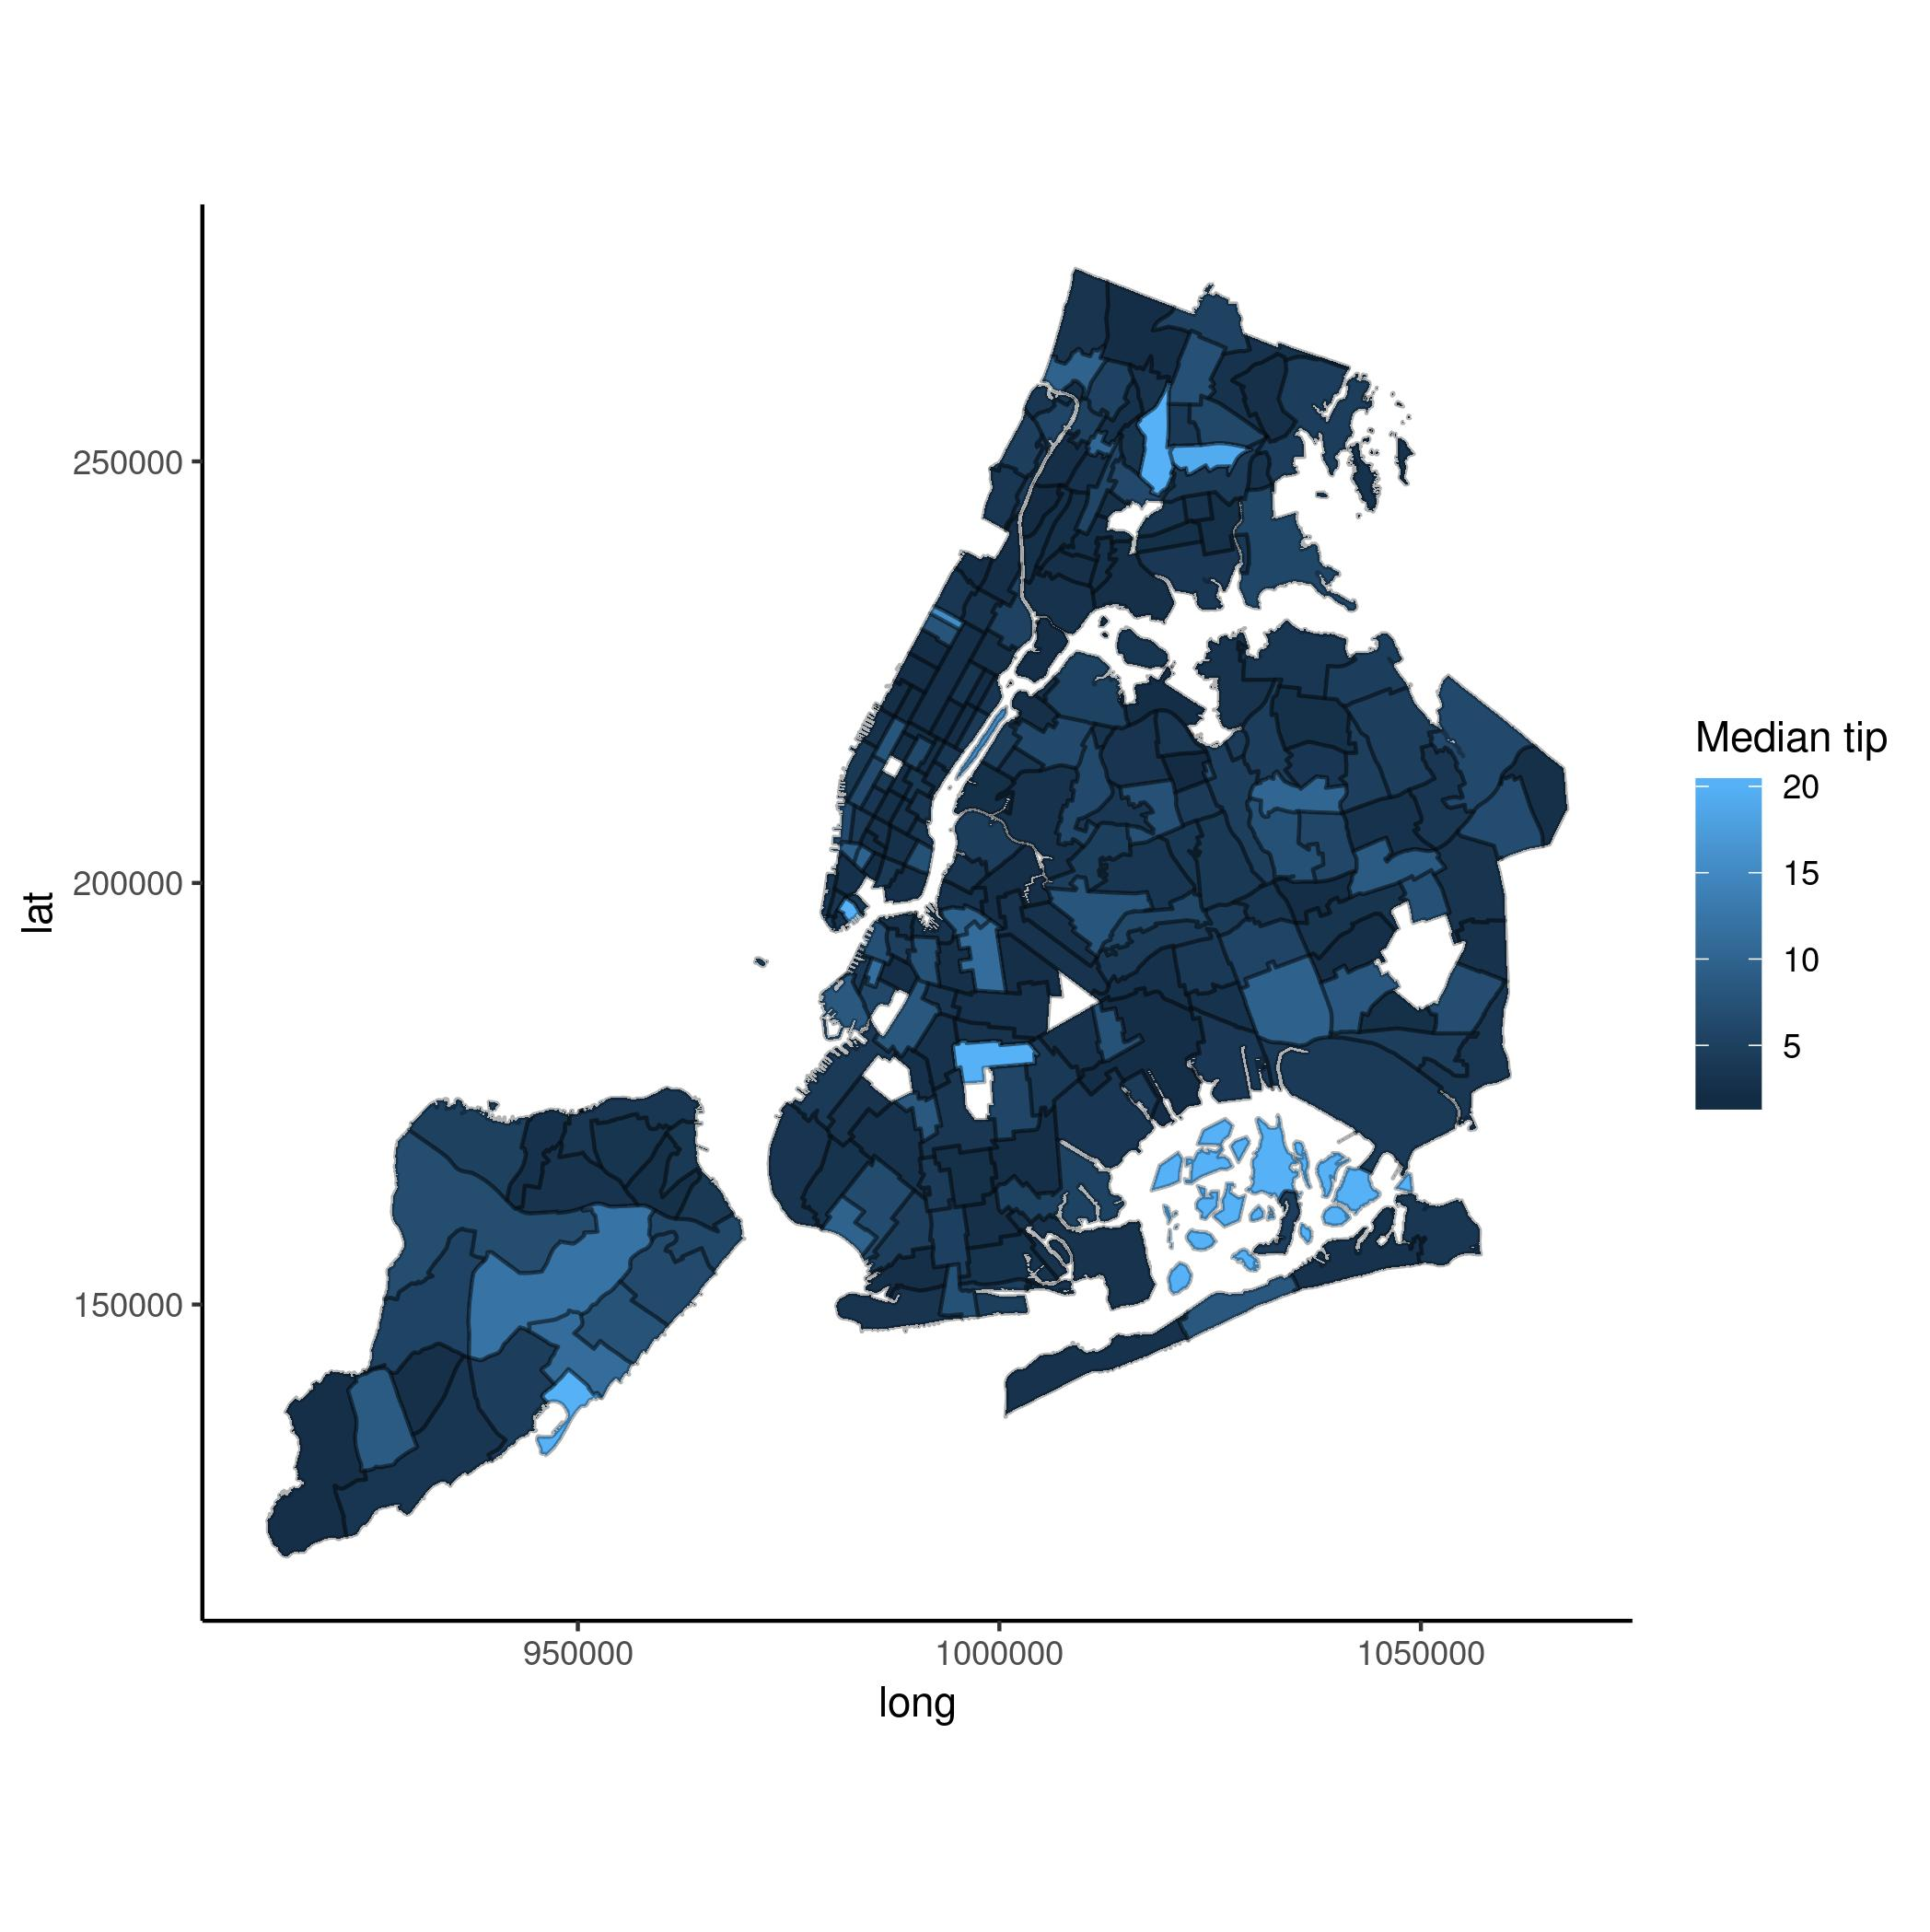
\includegraphics[width=.9\linewidth]{./plots/pickupTipMap.jpg}
\caption{\label{fig:org0de4c37}
Median tip by taxi pickup zone}
\end{figure}


\section{Modelling tips}
\label{sec:orgb0bdedc}

In this section I will build a model to predict the tip given
for a taxi ride. The main objective of this model is to give
users a recommendation based on what amount to tip, based on
what clients with similar ride characteristics tipped

\subsection{A note on accuracy metrics}
\label{sec:org633cb90}
Both the root mean squared error (RMSE) and mean absolute precentage
error (MAPE) are used to evaluate the models.
For all the presented models, RMSE ranges between \$1.25 and \$1.4, while
MAPE is between 0.4\% and 0.5\%.
The mean tip is \$2.5 dollars, with a \$2.4 standard deviation. all this can
be interpreted as: the models tend to give predictions that are about \$1.3 off.
these results are as bad they can be. I am however conviced that these kind of
accuracy metrics are also quite bad at evaluating the performance of
the models in our particular business case, specially considering how noisy
are the relationships in the data.
Are we more interested in recommending to the customer the actual amount
she is going to tip, or are we interested in providing her a summary of what
other customers in similar situations? I personally believe the later is more
interesting. As such, models will be evaluated plotting the distributions of the
actual data as well as the predictions given by the model.

\subsection{Linear models}
\label{sec:orgcfea1f5}
\begin{verbatim}
library(tidyverse)
library(reshape2)
library("glmnet")
library("lme4")

plotsFolder <- "plots"
modelsFolder <- "models"

boroughData <-  readRDS("boroughData.rds") %>%
    rename(DOLocationID = LocationID)

data <- readRDS("taxiDataFinal.rds") %>%
    filter(trip_distance > 0) %>%
    left_join(boroughData, by = "DOLocationID") %>%
    drop_na

discreteTipWeight <- data$tip_amount %>%
    sapply(
        function (x) {
            if (x %in% c(1.0, 2.0, 3.0, 5.0)) 1.3
            else 1
        })

evaluation <- function(model, testData) {
    mu <- data$tip_amount %>% log %>%  mean
    sigma <- data$tip_amount %>% log %>% sd
    prediction0 <- predict(model, testData)
    evaluation0 <- testData %>% select(tip_amount) %>%
        mutate(prediction = prediction0) %>%
        mutate(tip_amount = exp(mu + (tip_amount * sigma)),
               prediction = exp(mu + (prediction * sigma))) %>%
        mutate(error = tip_amount - prediction) %>%
        mutate(mape = abs(error / tip_amount),
               rmse = error * error)
    evaluation0 %>% summary
    mape <- evaluation0$mape %>% mean
    rmse <- evaluation0$rmse %>% mean %>% sqrt

    errorDistribution <- ggplot(data = evaluation0, aes(error)) + geom_histogram(bins = 100)

    print("evaluation metrics")
    print(paste("mape is:", mape))
    print(paste("rmse is:", rmse))

    list(evaluationFrame = evaluation0, errorDistrbution = errorDistribution,
         rmse = rmse, mape = mape)
}

posteriorPredictivePlot <- function(evaluation, name) {
    toPlot <- evaluation$evaluationFrame %>%
        select(tip_amount, prediction) %>%
        melt
    print(toPlot %>% head)
    print(paste(plotsFolder, name, sep = "/"))
    plot <- ggplot(toPlot, aes(value, fill = variable)) +
        geom_histogram(bins = 100, position = "identity", alpha = 0.3) + xlim(NA, 10)
    ggsave(paste(plotsFolder, name, sep = "/"), plot)
    plot
}

## mutate and select variables to fit             
## dataToFit <- data %>%
##     filter(trip_distance > 0) %>% 
##     ## change numeric variables
##     mutate_at(
##         .vars = vars(trip_distance, fare_amount,
##                      tip_amount, rideTime),
##         .funs = function(x) x %>% log %>% scale) %>%
##                                         # change factor variables
##     mutate_at(
##         .vars = vars(passenger_count, RatecodeID,
##                      store_and_fwd_flag, payment_type,
##                      weekEnd, tollPaid, borough),
##         .funs = as.factor) %>%
##     select(
##         trip_distance, fare_amount, tip_amount, rideTime,
##         passenger_count, RatecodeID, store_and_fwd_flag,
##         weekEnd, tollPaid, borough, payment_type)
## dataToFit %>% saveRDS("dataToFit.rds")
dataToFit <- readRDS("dataToFit.rds")
## split data in train and test sets
## 0.8 of the data will be used to train, remainder to test
trainSize <- floor(0.8 * nrow(dataToFit))
trainSize
## set the seed to make your partition reproducible
set.seed(123)
trainIndex <- sample(seq_len(nrow(dataToFit)), size = trainSize)
dataToFit %>% head
train <- dataToFit[trainIndex, ]
test <- dataToFit[-trainIndex, ]

model0 <- lm(tip_amount ~ -1 + borough + RatecodeID, data = train)
evaluation0 <- evaluation(model0, test)
posteriorPredictive <- evaluation0 %>% posteriorPredictivePlot(
                                           "evaluation0PosteriorPredictive.jpg")

model1 <- lm(tip_amount ~ -1 + borough +
                 RatecodeID + tollPaid + store_and_fwd_flag +
                 fare_amount + trip_distance,
             data = train)
evaluation1 <- model1 %>% evaluation(test)
posteriorPredictive <- evaluation1 %>% posteriorPredictivePlot(
                                           "evaluation1PosteriorPredictive.jpg")

model2 <- lm(tip_amount ~ -1 +
                 RatecodeID + tollPaid + store_and_fwd_flag +
                 fare_amount + trip_distance + borough,
             data = train)

evaluation2 <- model2 %>% evaluation(test)
posteriorPredictive2 <- evaluation2 %>% posteriorPredictivePlot(
                                            "evaluation2PosteriorPredictive.jpg")

x <- model.matrix(tip_amount ~ -1 + RatecodeID + tollPaid + store_and_fwd_flag +
                 fare_amount + trip_distance + borough, dataToFit[trainIndex,])
y <- dataToFit[trainIndex,] %>% select(tip_amount) %>% as.matrix

model3cv <- cv.glmnet(x = x, y = y, nfolds = 5, lambda = seq(2, 100, 2),
                    alpha = 0, family = "gaussian")

model3 <- glmnet(x = x, y = y, lambda = model3cv$lambda.min,
                 alpha = 0.1, family = "gaussian")

modelsFolder <- "models"
model3 %>% saveRDS(paste(modelsFolder, "model3.rds", sep = '/'))
model3 <- readRDS(paste(modelsFolder, "model3.rds", sep = '/'))

prediction3 <- predict(
    model3,
    newx = model.matrix(
        tip_amount ~ -1 + RatecodeID + tollPaid + store_and_fwd_flag +
            fare_amount + trip_distance + borough,
        dataToFit[-trainIndex,]))

evaluation3 <- list(evaluationFrame = test %>% select(tip_amount) %>%
                        mutate(prediction = prediction3))
posteriorPredictive3 <- evaluation3 %>% posteriorPredictivePlot(
                                            "evaluation3PosteriorPredictive.jpg")

model4 <- lmer(tip_amount ~ -1 + (1 | borough) + trip_distance +
                   store_and_fwd_flag + (0 + fare_amount| borough), data = train)

evaluation4 <- model4 %>% evaluation(test)
posteriorPredictive4 <- evaluation4 %>% posteriorPredictivePlot(
                                            "evaluation4PosteriorPredictive.jpg")

model5 <- lmer(tip_amount ~ -1 +
                   (1 | RatecodeID) + (1 | tollPaid) + (1 | store_and_fwd_flag) +
                   fare_amount + (1 + fare_amount | borough) + trip_distance,
               data = train, weights = discreteTipWeight[trainIndex])

evaluation5 <- model5 %>% evaluation(test)
posteriorPredictive5 <- posteriorPredictivePlot(
    evaluation5,
    "evaluation5PosteriorPredictive.jpg")

model6 <- lmer(tip_amount ~ -1 +
                   (1 | RatecodeID) + (1 | tollPaid) + (1 | store_and_fwd_flag) +
                   fare_amount +
                   (1 + fare_amount | payment_type),
               data = train, weights = discreteTipWeight[trainIndex])

evaluation6 <- model6 %>% evaluation(test)
posteriorPredictive6 <- posteriorPredictivePlot(
    evaluation6,
    "evaluation6PosteriorPredictive.jpg")

\end{verbatim}

Our first linear model is fitted with only the \emph{borough} and \emph{RatecodeID}
dummy variables. This fit is quite bad, but is here just to find out how
this variables are effecting the model.

\begin{figure}[htbp]
\centering
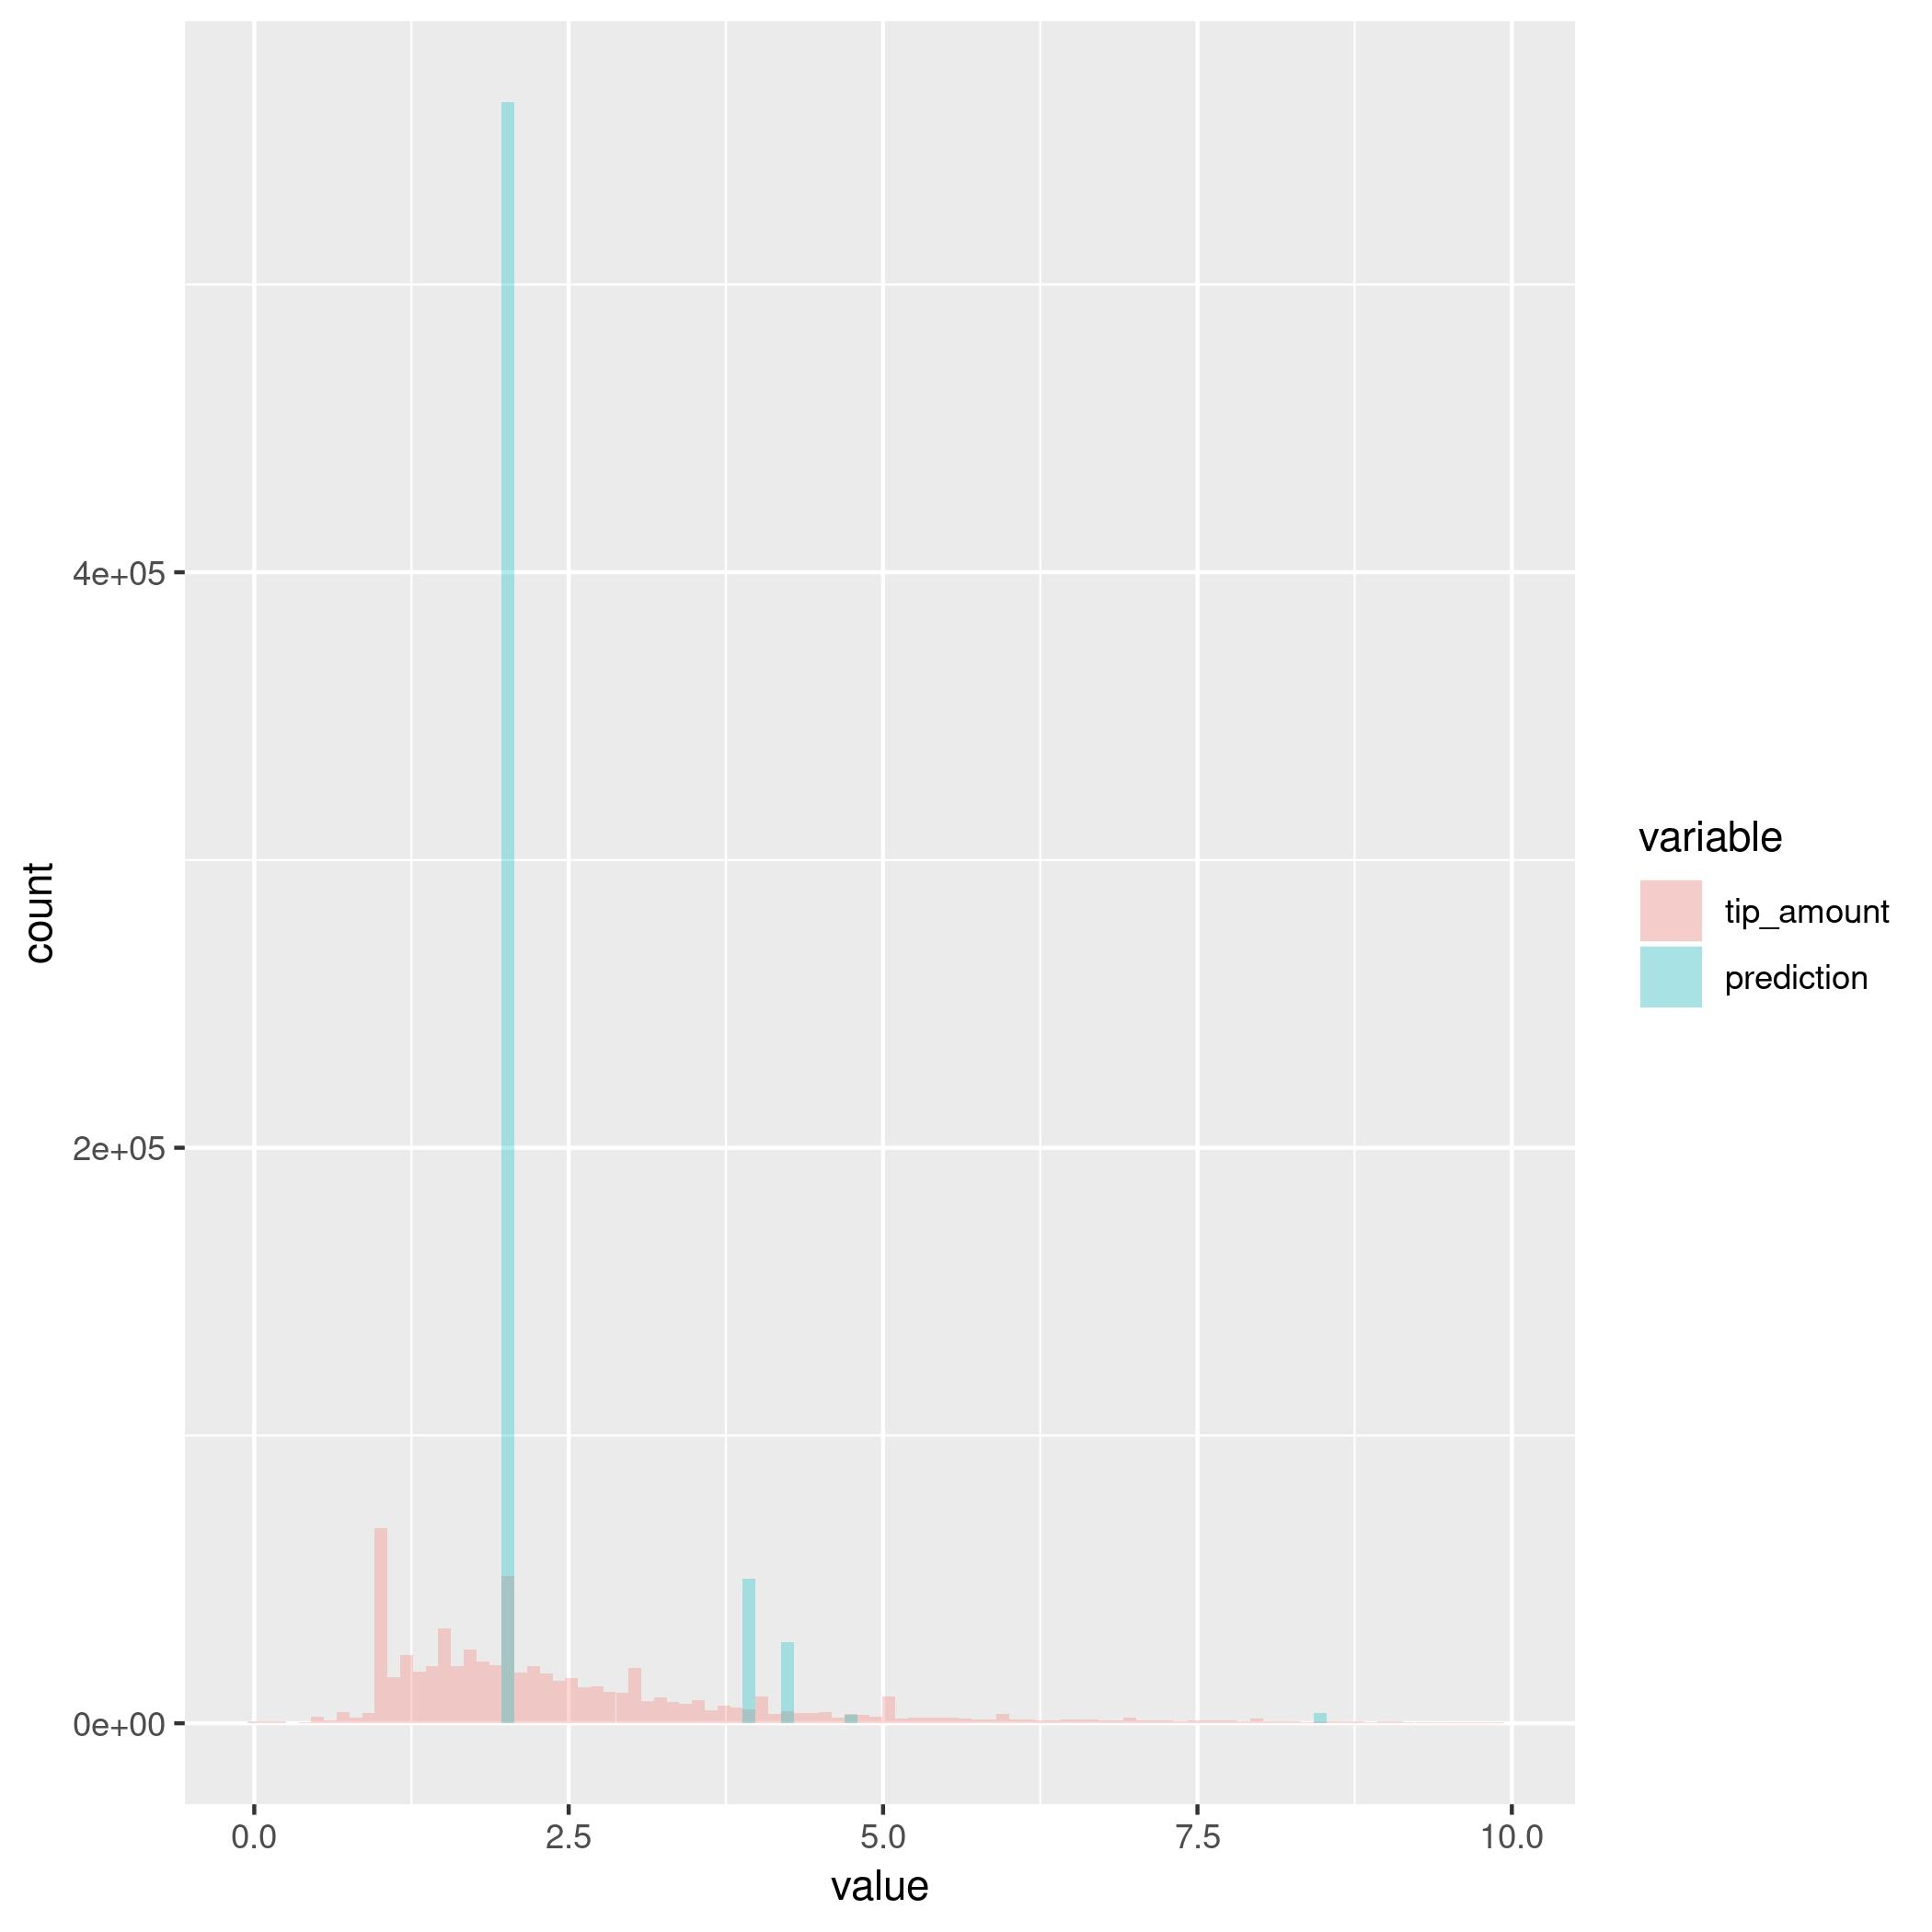
\includegraphics[width=.9\linewidth]{./plots/evaluation0PosteriorPredictive.jpg}
\caption{\label{fig:orgbf15125}
Posterior predictive evaluation}
\end{figure}

The next two models include \emph{trip\_distance} as well as \emph{fare\_amount} in
logarithms and normalized. As dummy variables \emph{RatecodeID}, \emph{tollPaid},
\emph{store\_and\_fwd\_flag} and drop off \emph{borough} are selected as they are a
subset is representative of all the discrete variables availabel. A better
approach would have been to take all the discrete variables, and transform
with PCA, to avoid the dimensionality problem that justified choosing only
a subset. On the other hand, the implemented approach improves the
interpretability of the models.

This next plot displays the results of a simple linear regression.
the on first sight, it is obvious that the models is doing a good job
of approximating the general distribution, but seems to have problems
picking up the spikes that are present on the round tips (tips of \$1, \$2, etc)
as well as the left tail.

\begin{figure}[htbp]
\centering
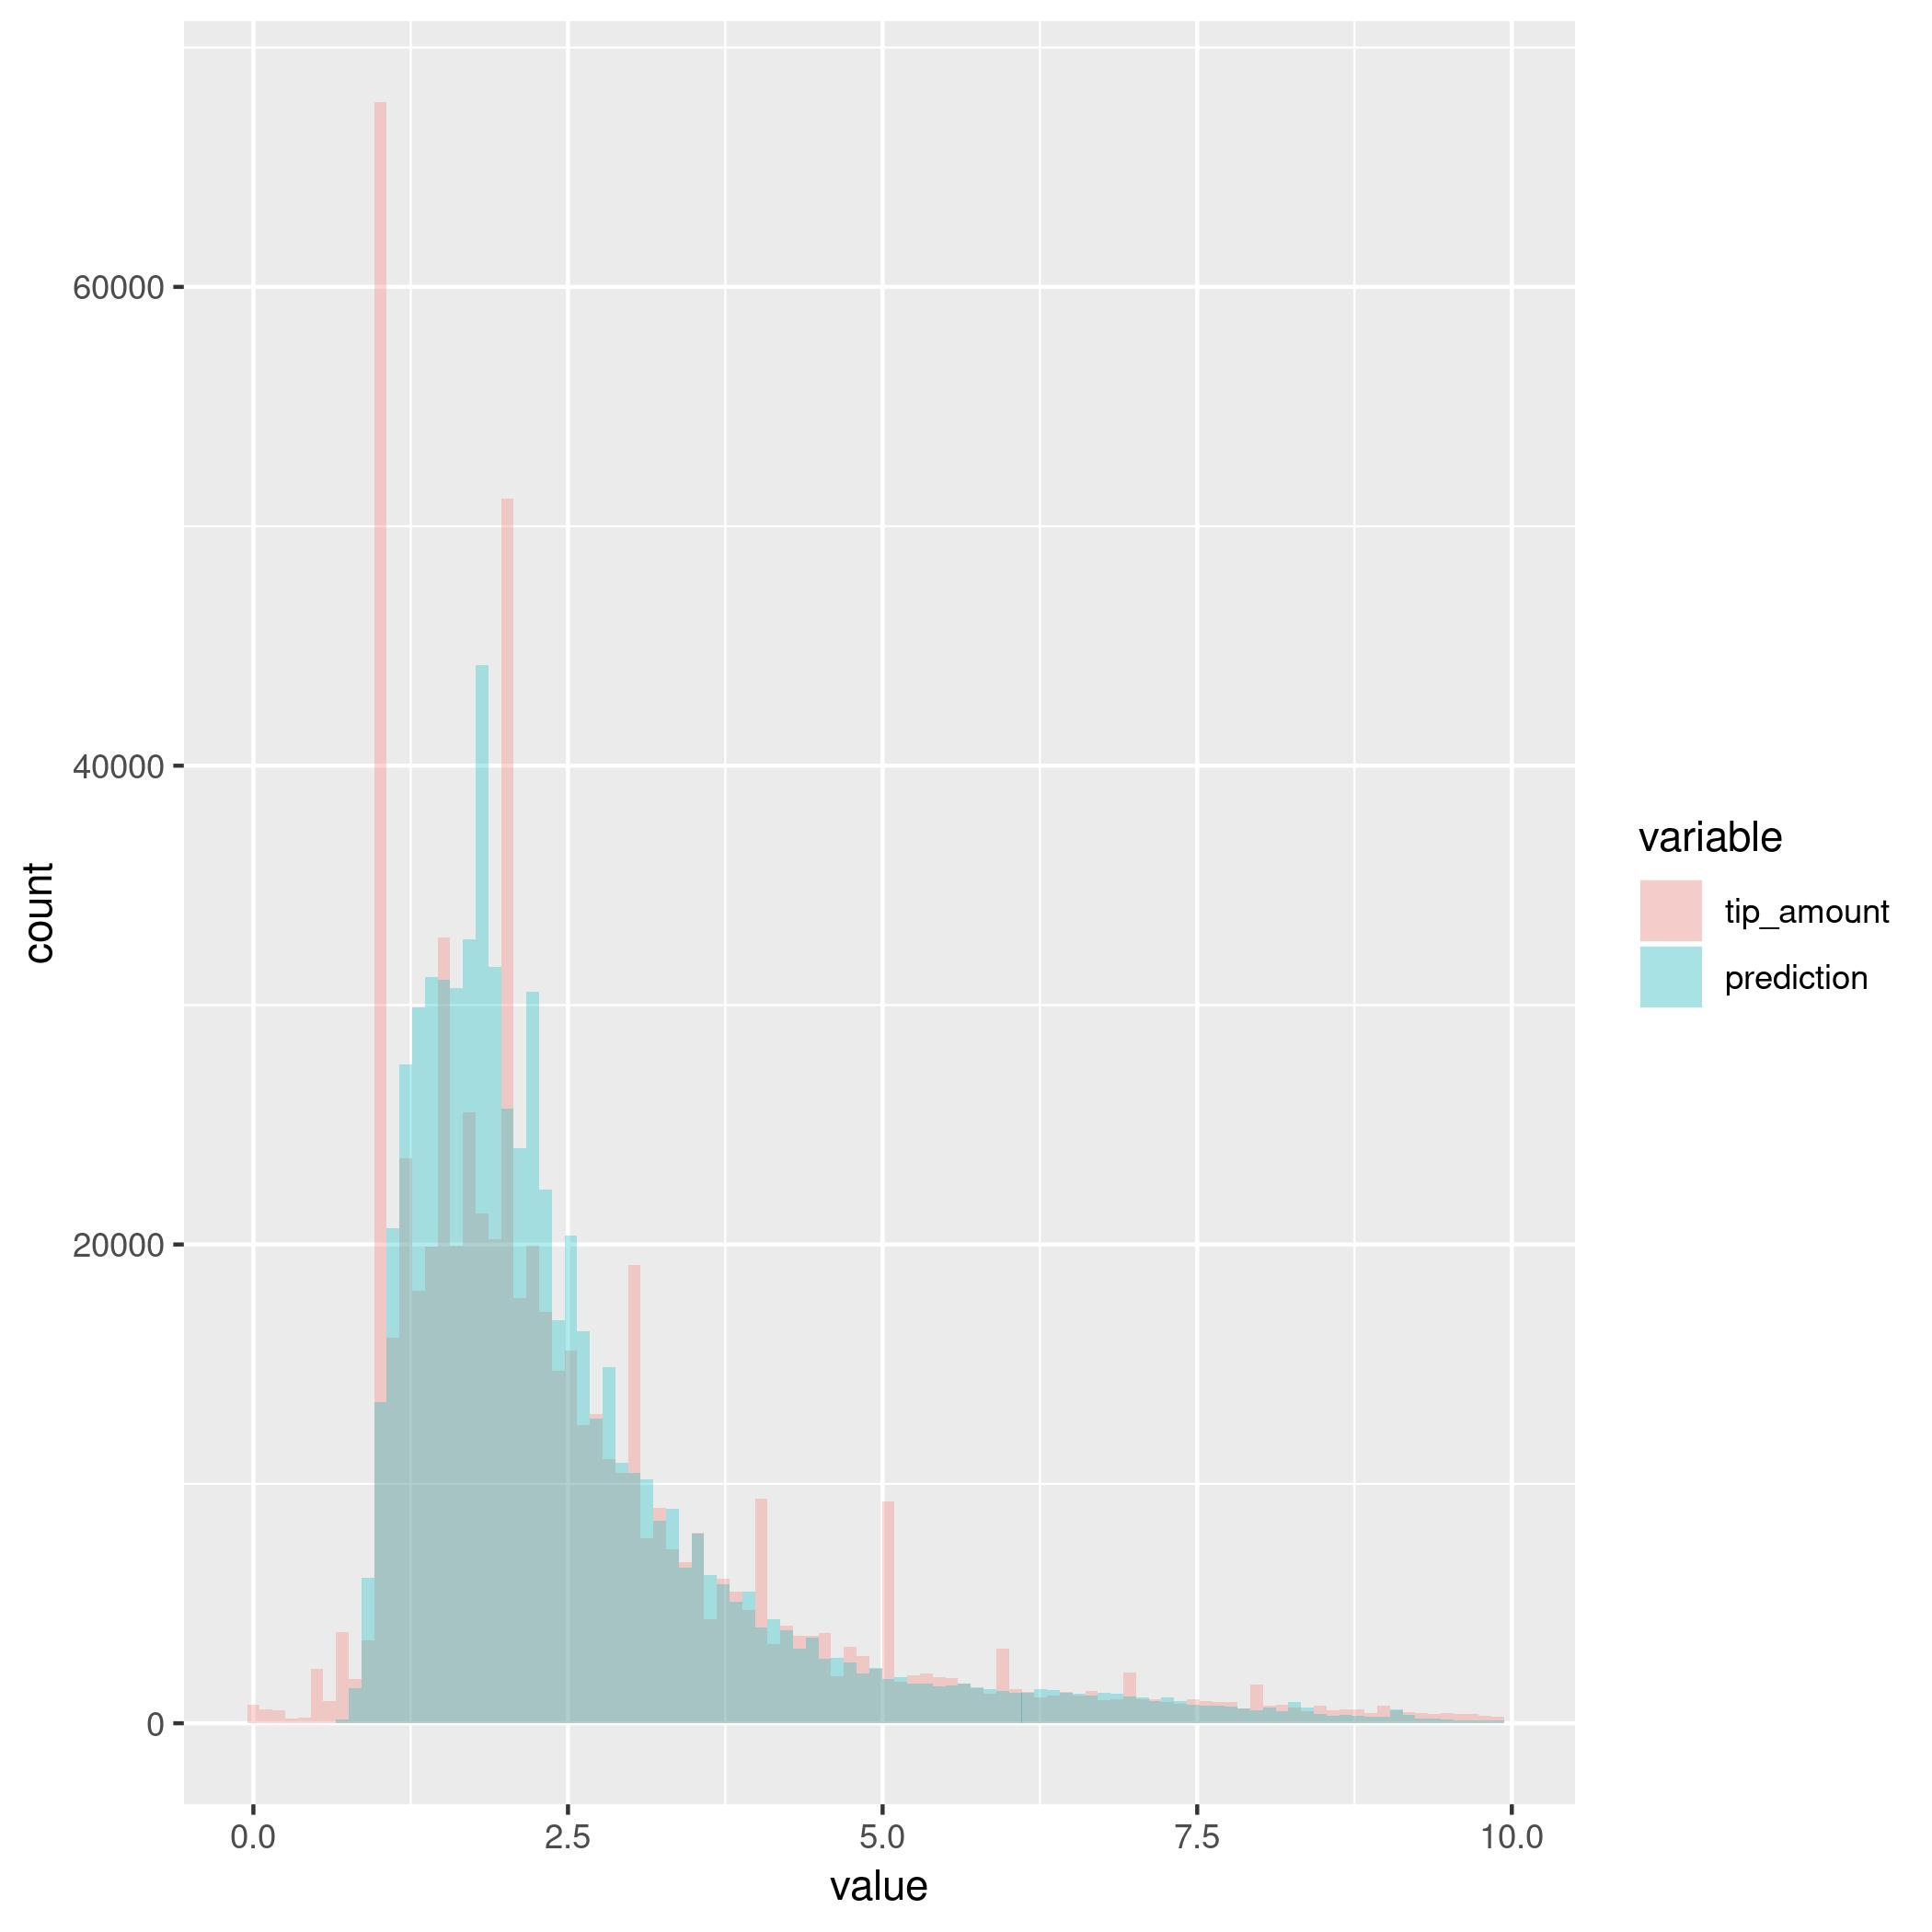
\includegraphics[width=.9\linewidth]{./plots/evaluation1PosteriorPredictive.jpg}
\caption{\label{fig:org7f87f81}
Posterior predictive evaluation}
\end{figure}

The most interesting failure of the previous model would be the round tips.
First, some clients seem to be giving a tip of \$1 regardless of other
characteristics of the trip. Furthermore, there also seems to be a tendency
to give round tips.
To approximate this behaviour, the next model is a weighted linear model,
were the round values have more weight than the remaining. As such, the
predictive posterior of this model is tighter to the original data:
first, it is approximates the \$2 spike quite well.
But it also generates two spikes between the actuals \$1 and \$2. This is
interesting, because it indicates that we do not have enough information
to approximate linearly the spike at \$1 and the remaining error at the
spike at \$2. This would be probably one of the most interesting models to
actually implement in a production evironment.

\begin{figure}[htbp]
\centering
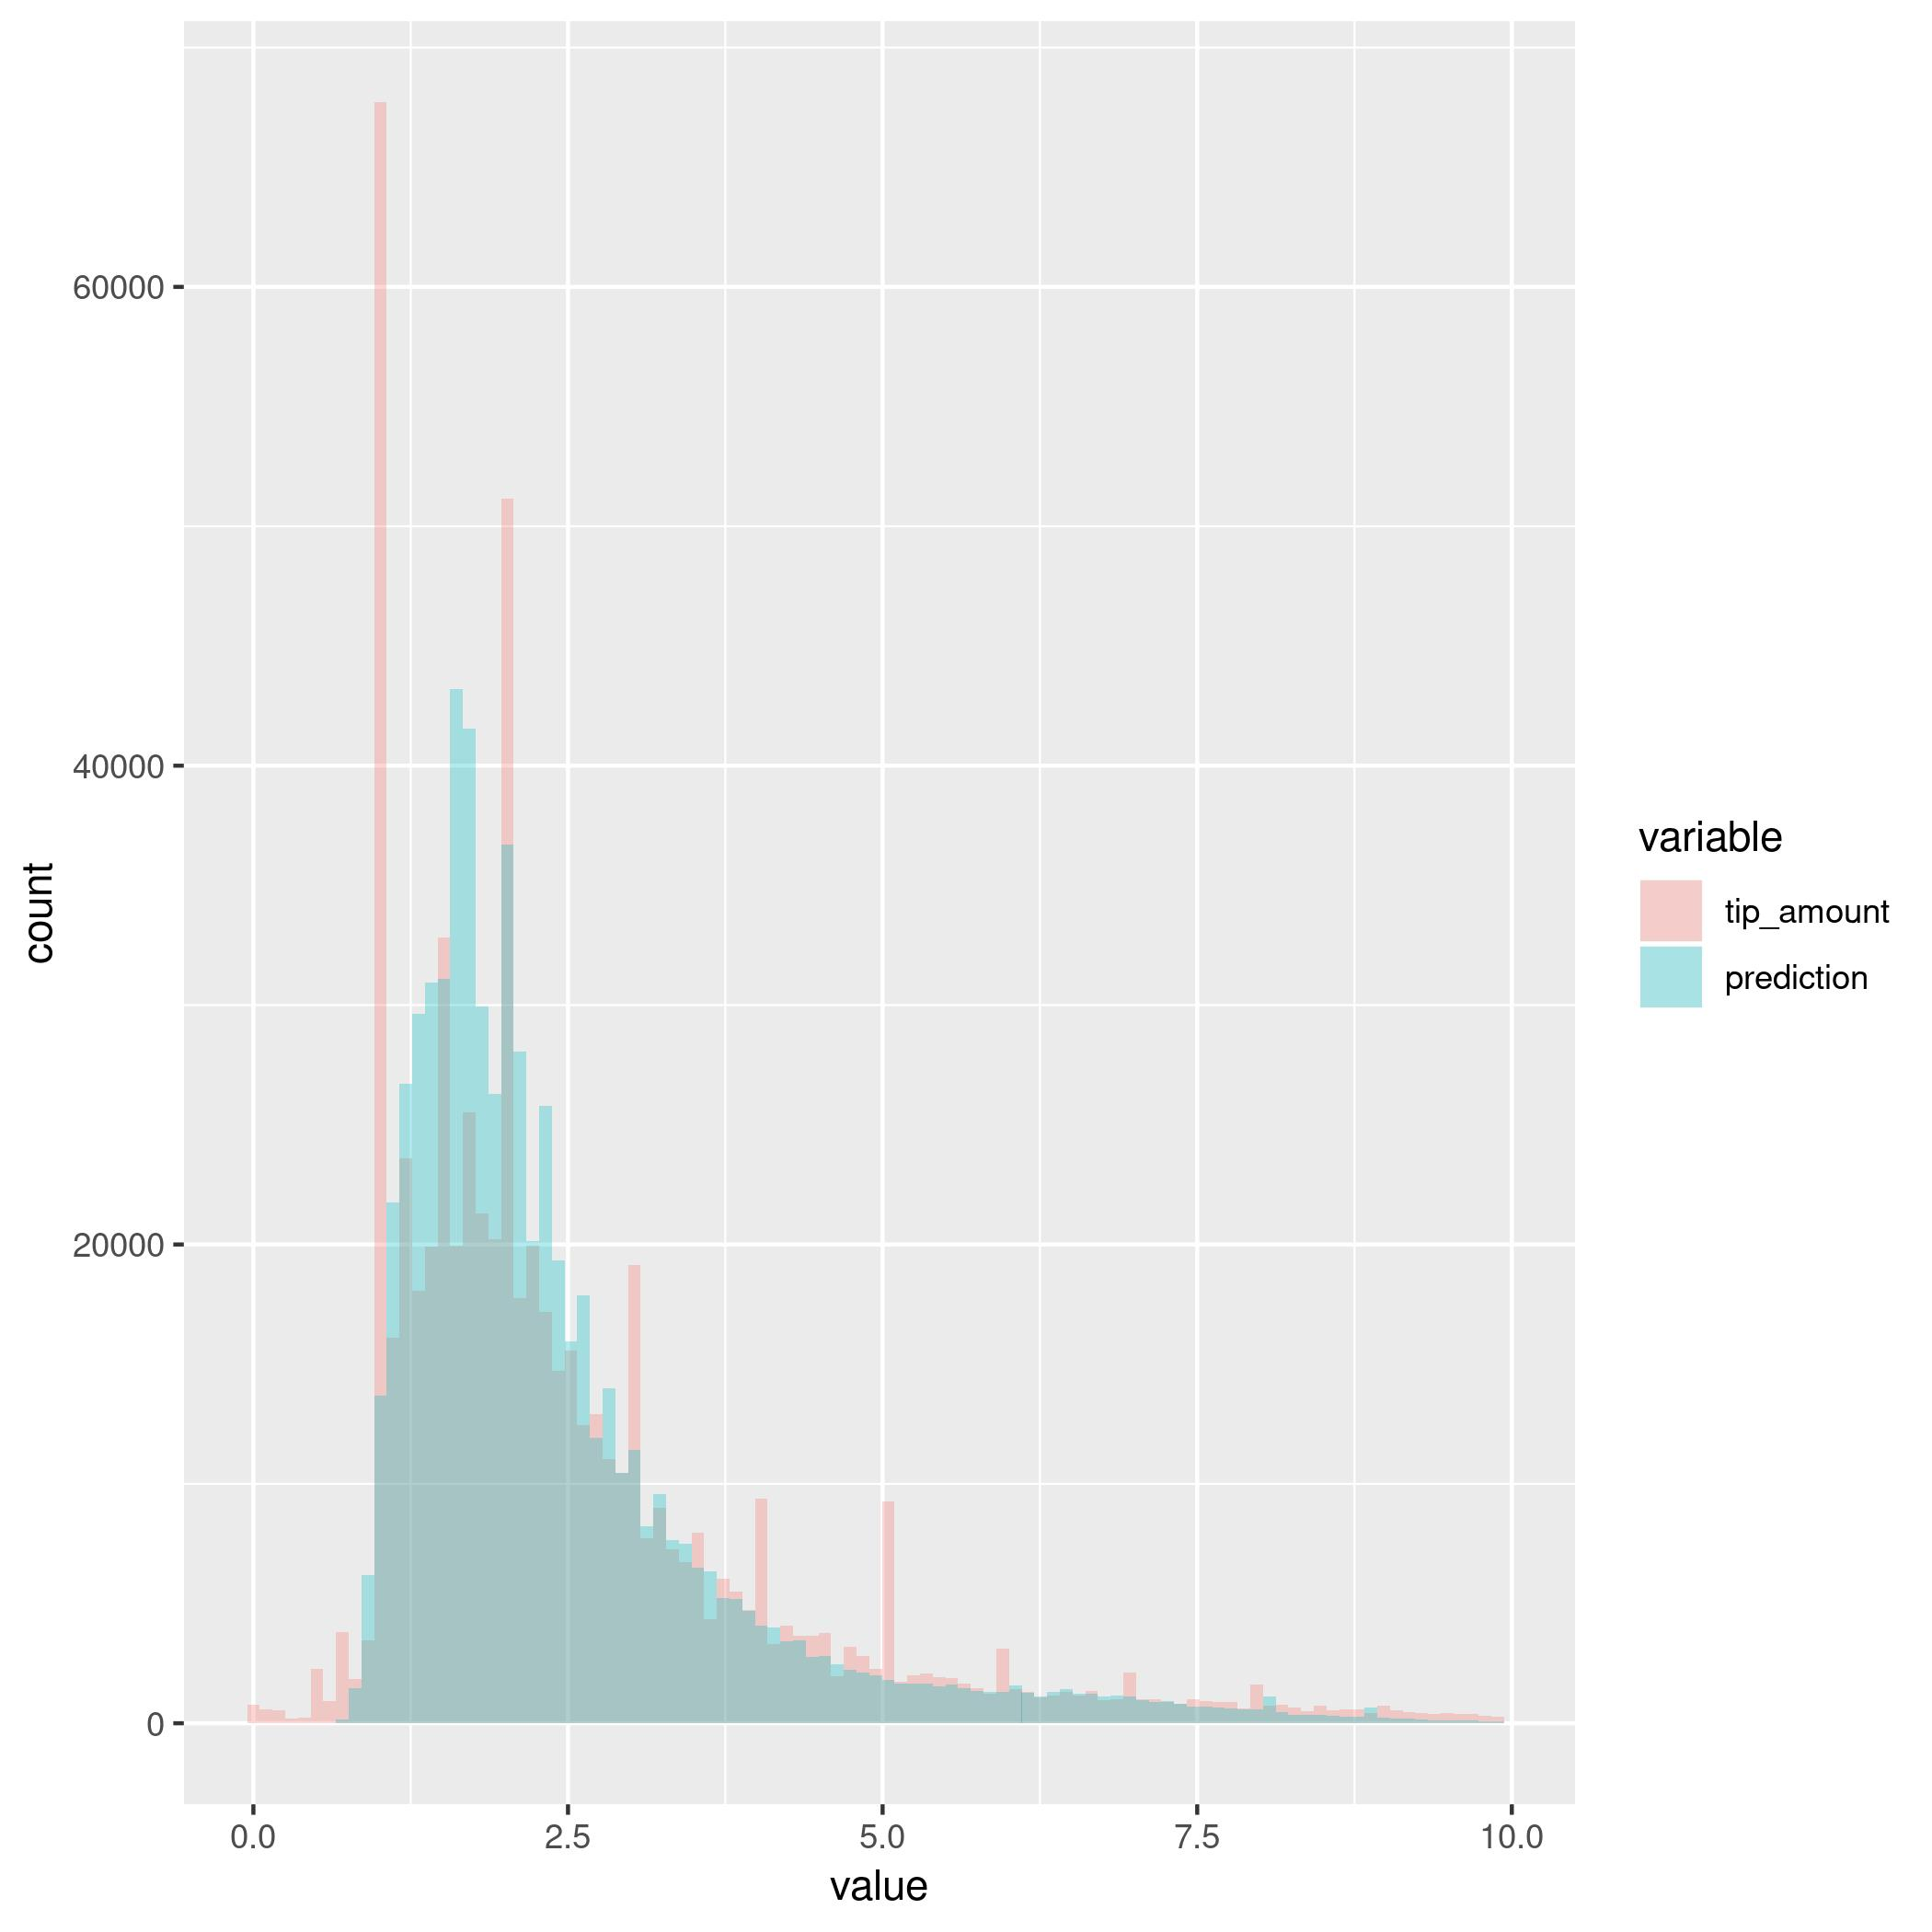
\includegraphics[width=.9\linewidth]{./plots/evaluation2PosteriorPredictive.jpg}
\caption{\label{fig:org0c33e25}
Posterior predictive evaluation}
\end{figure}

the next plot showcases the results for a linear regression with
regularization. this model fits the data quite poorly.

\begin{figure}[htbp]
\centering
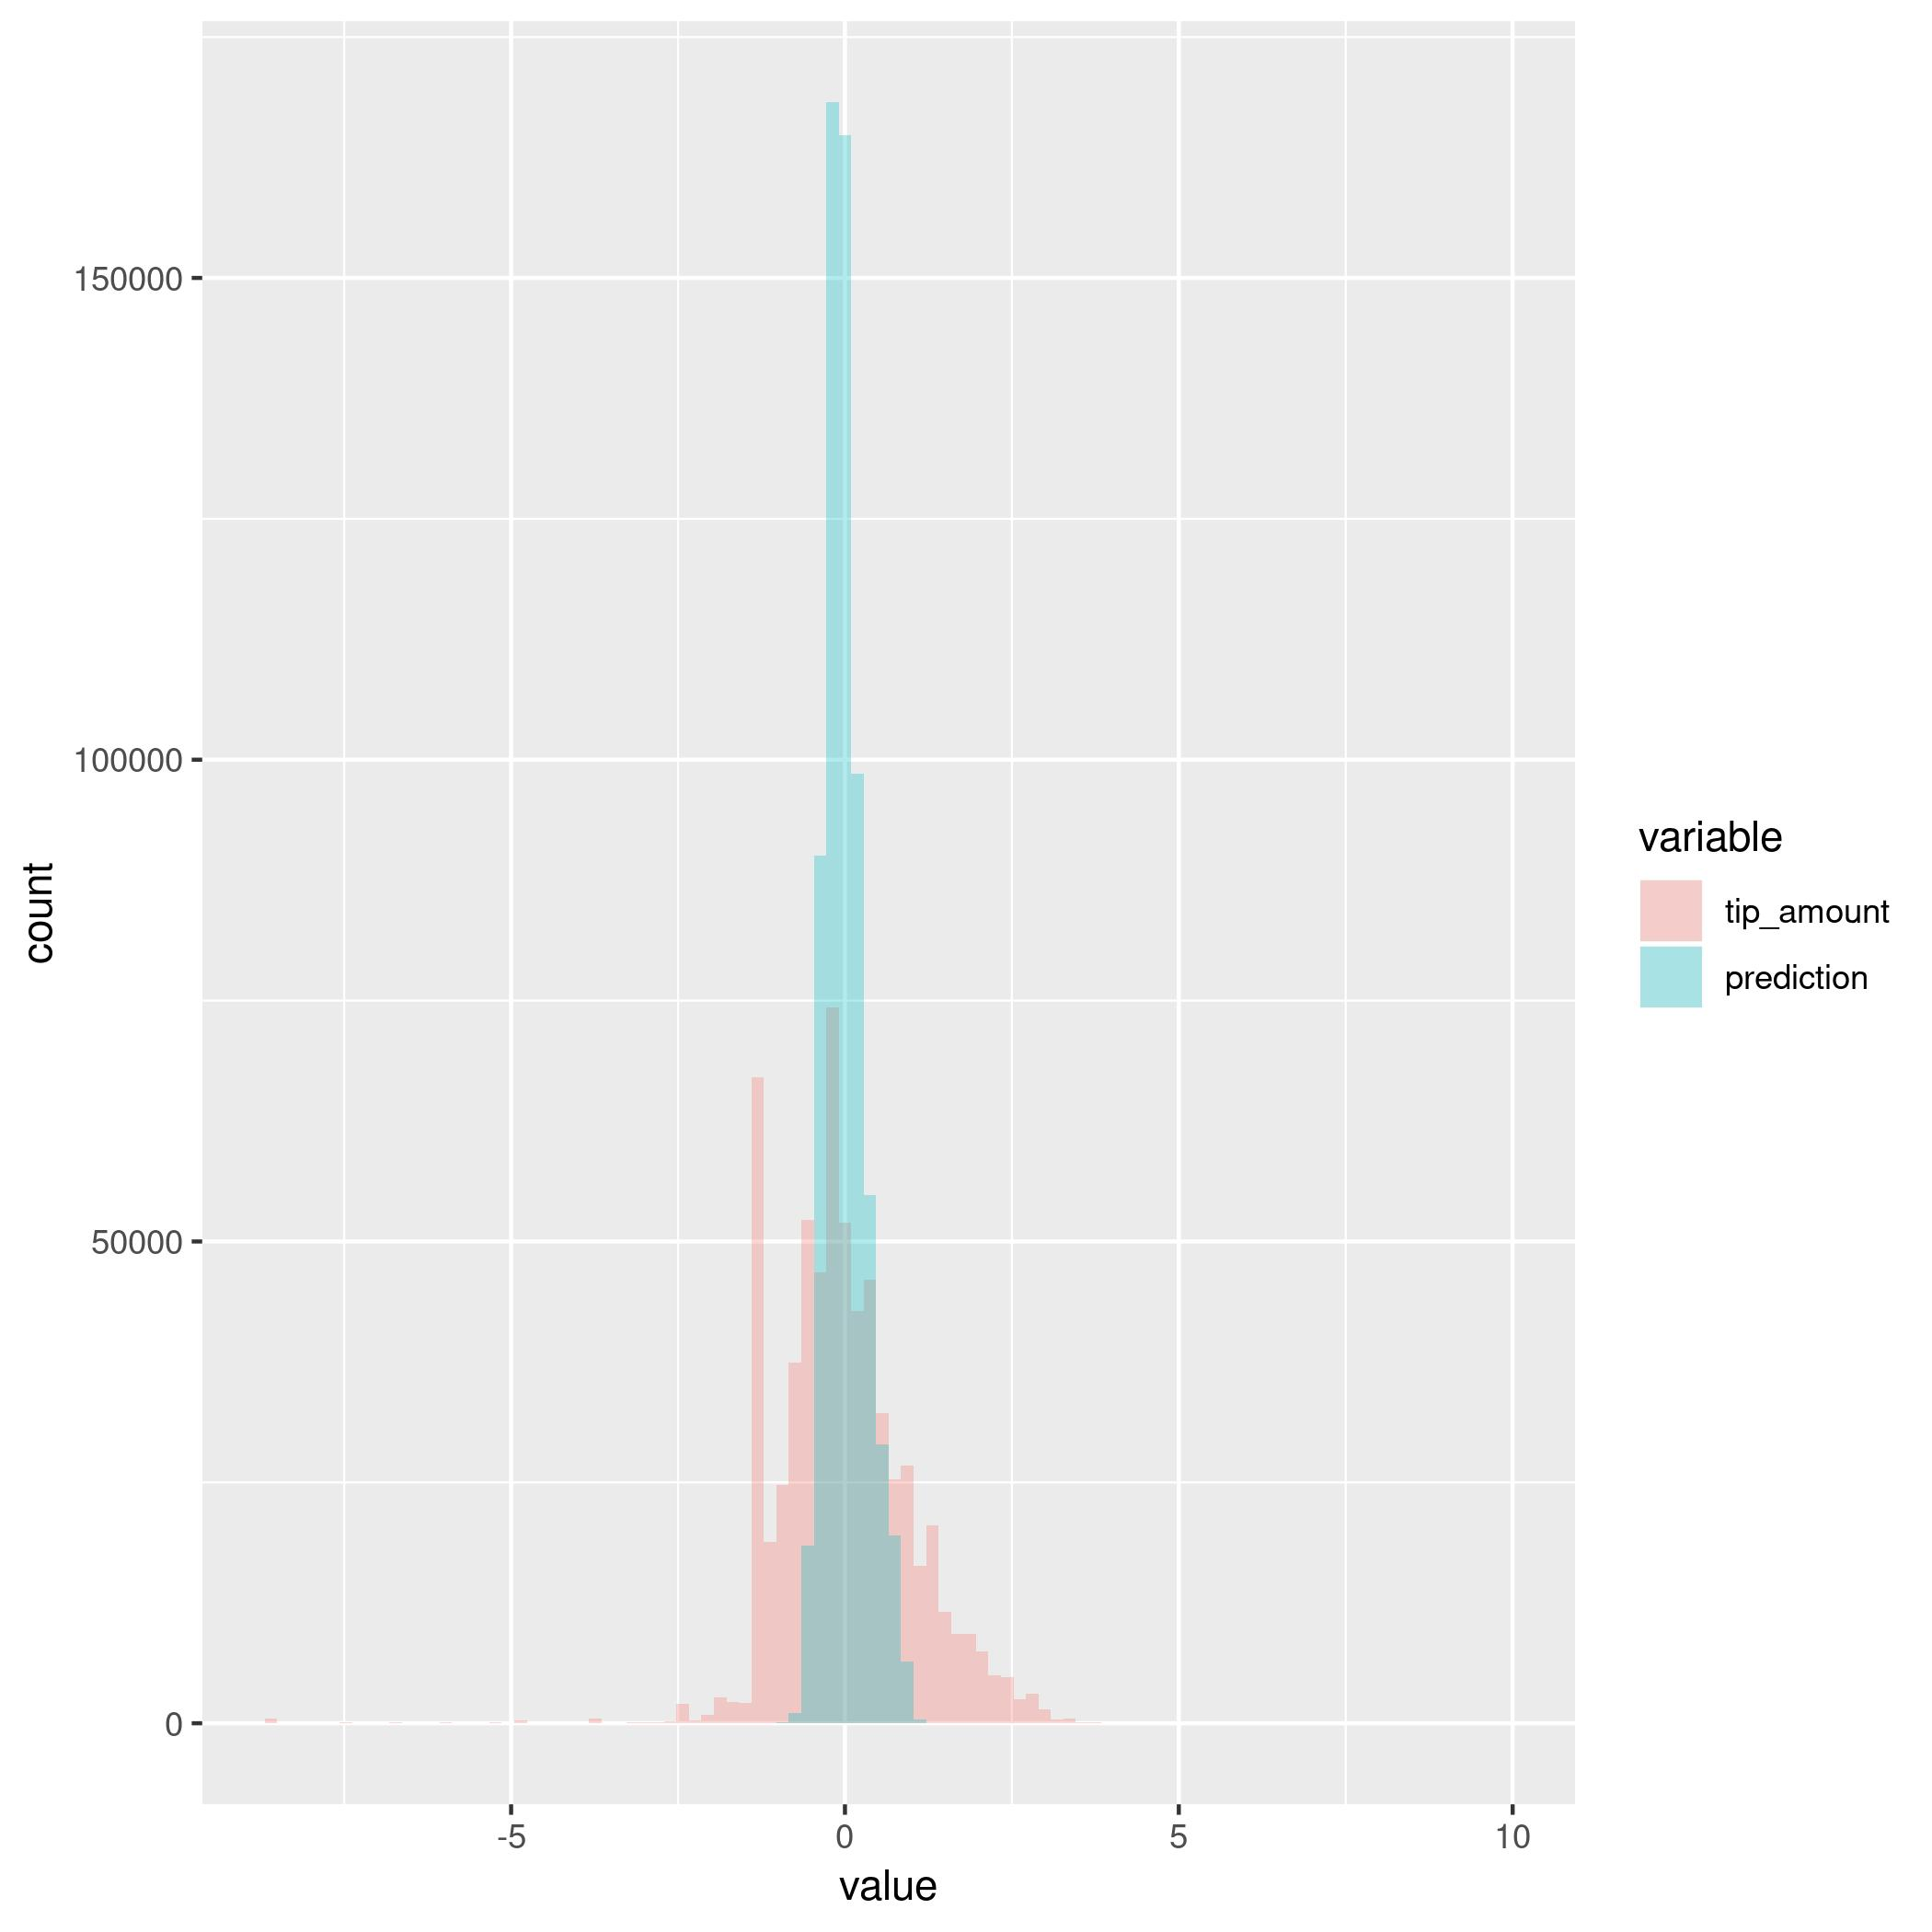
\includegraphics[width=.9\linewidth]{./plots/evaluation3PosteriorPredictive.jpg}
\caption{\label{fig:orgff972ec}
Posterior predictive evaluation}
\end{figure}

Finally, in order to approximate better some non linearities, the
previous models are extended with interaction terms between \emph{borough}
and \emph{fare\_amount} in a mixed linear model. This is, we allow that for
each \emph{borough}, the \emph{fare\_amount} variable has a different slope term.
As in the previous linear model, both regular and weighted linear models
are fitted. The fit is quite similar than before, but this model seems
to better approximate the spikyness of the data.

\begin{figure}[htbp]
\centering
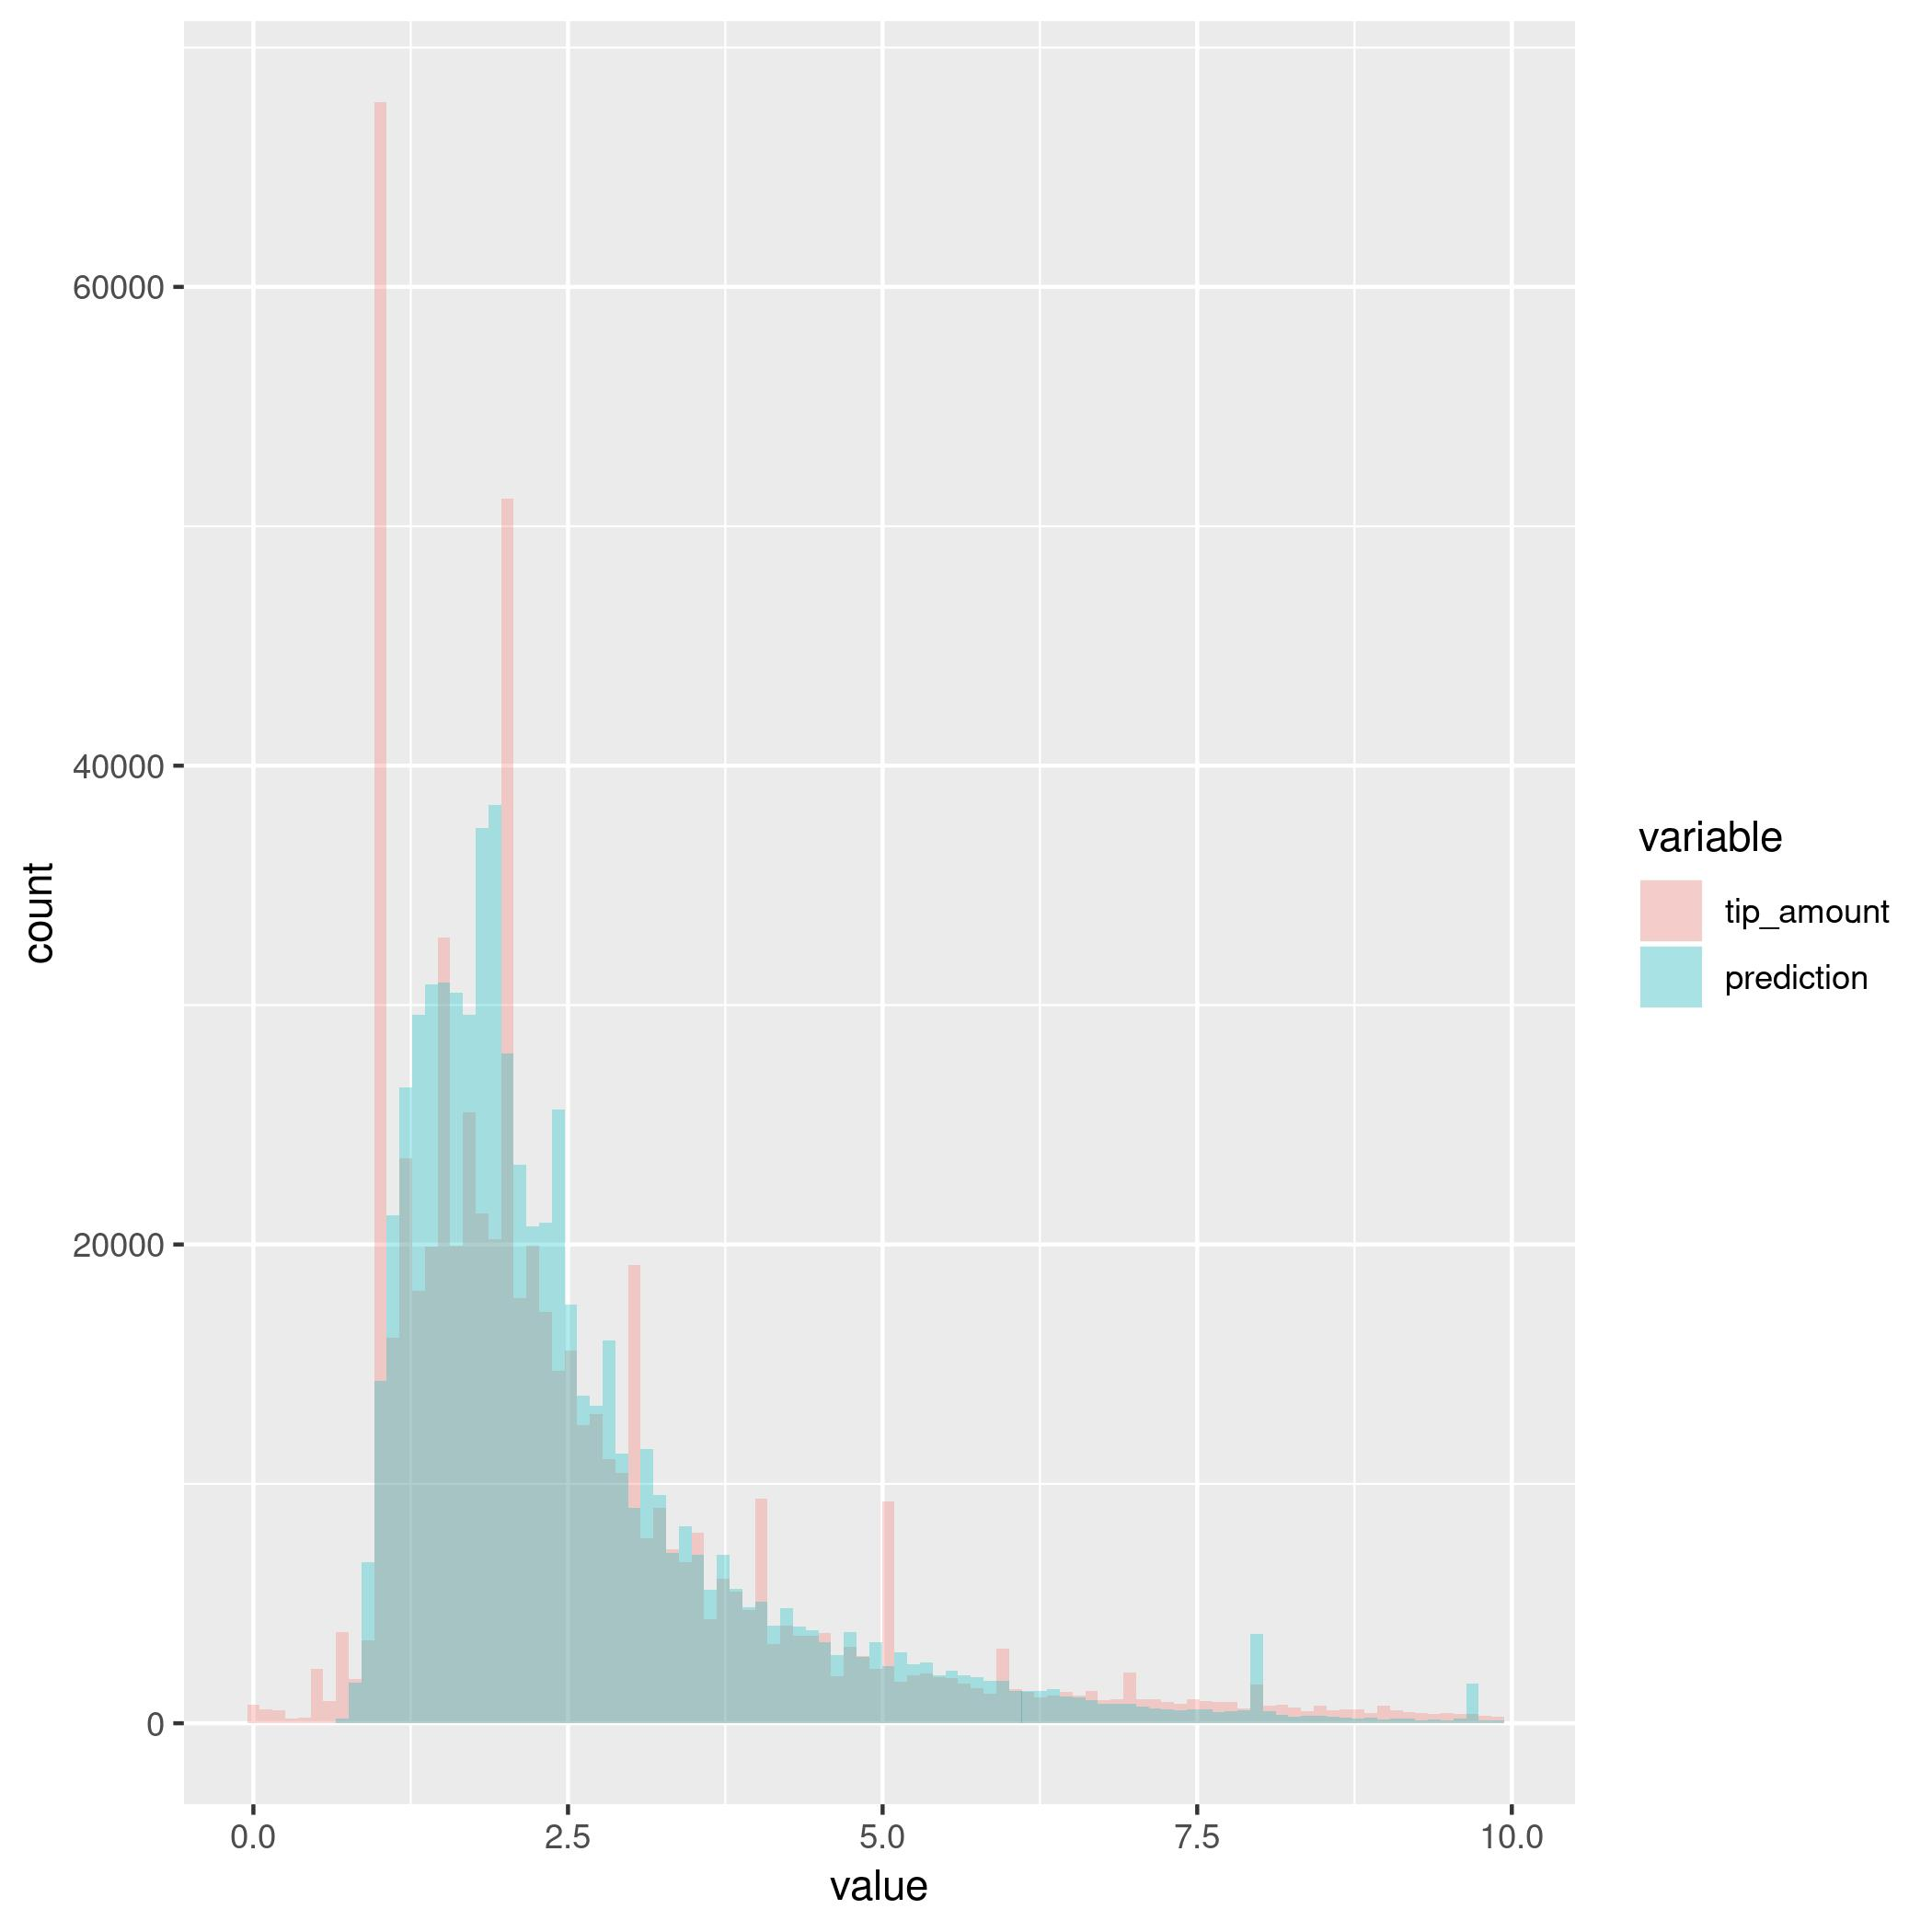
\includegraphics[width=.9\linewidth]{./plots/evaluation4PosteriorPredictive.jpg}
\caption{\label{fig:org8872adb}
Posterior predictive evaluation}
\end{figure}

\begin{figure}[htbp]
\centering
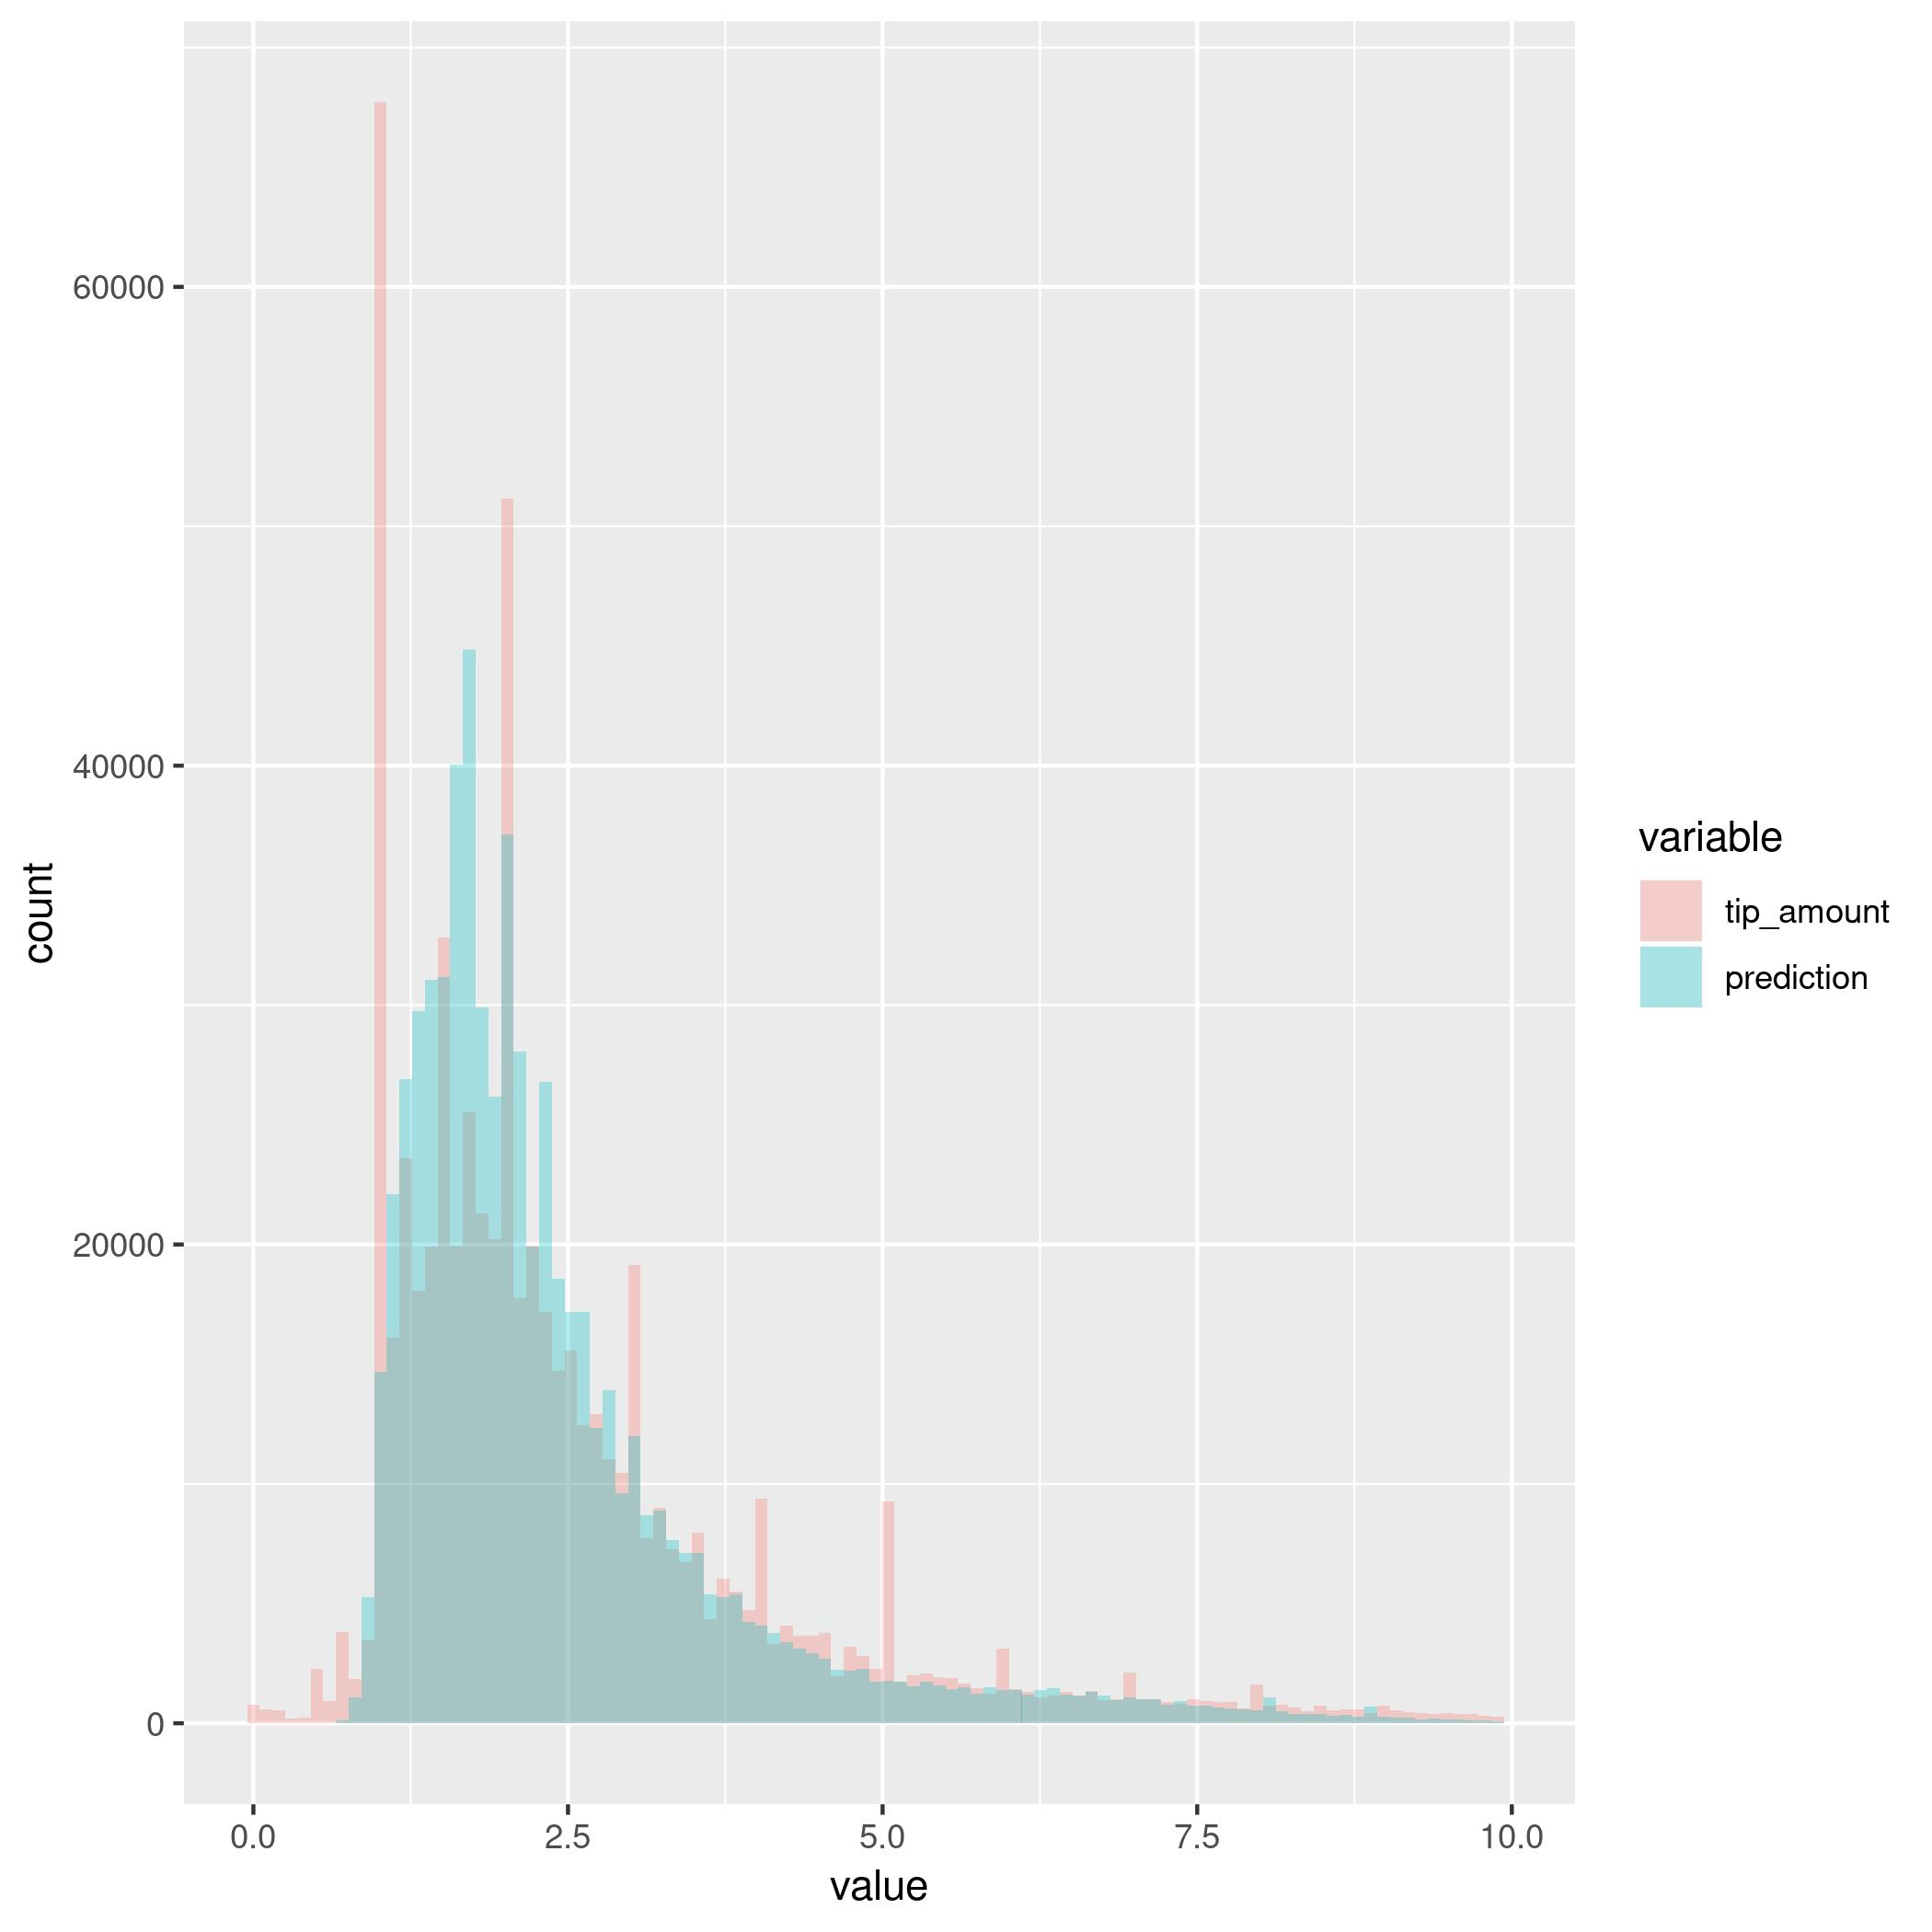
\includegraphics[width=.9\linewidth]{./plots/evaluation5PosteriorPredictive.jpg}
\caption{\label{fig:org9b8f82e}
Posterior predictive evaluation}
\end{figure}


\subsection{Random forest}
\label{sec:org892cd8a}
\begin{verbatim}
library(tidyverse)
library(reshape2)
library("randomForest")

evaluation <- function(model, testData) {
    mu <- data$tip_amount %>% log %>%  mean
    sigma <- data$tip_amount %>% log %>% sd
    prediction0 <- predict(model, testData)
    evaluation0 <- testData %>% select(tip_amount) %>%
        mutate(prediction = prediction0) %>%
        mutate(tip_amount = exp(mu + (tip_amount * sigma)),
               prediction = exp(mu + (prediction * sigma))) %>%
        mutate(error = tip_amount - prediction) %>%
        mutate(mape = abs(error / tip_amount),
               rmse = error * error)
    evaluation0 %>% summary
    mape <- evaluation0$mape %>% mean
    rmse <- evaluation0$rmse %>% mean %>% sqrt

    errorDistribution <- ggplot(data = evaluation0, aes(error)) + geom_histogram(bins = 100)

    print("evaluation metrics")
    print(paste("mape is:", mape))
    print(paste("rmse is:", rmse))

    list(evaluationFrame = evaluation0, errorDistrbution = errorDistribution,
         rmse = rmse, mape = mape)
}

posteriorPredictivePlot <- function(evaluation, name) {
    toPlot <- evaluation$evaluationFrame %>%
        select(tip_amount, prediction) %>%
        melt
    print(toPlot %>% head)
    print(paste(plotsFolder, name, sep = "/"))
    plot <- ggplot(toPlot, aes(value, fill = variable)) +
        geom_histogram(bins = 100, position = "identity", alpha = 0.3) + xlim(NA, 10)
    ggsave(paste(plotsFolder, name, sep = "/"), plot)
    plot
}


plotsFolder <- "plots"
modelsFolder <- "models"

boroughData <-  readRDS("boroughData.rds") %>%
    rename(DOLocationID = LocationID)

data <- readRDS("taxiDataFinal.rds") %>%
    filter(trip_distance > 0) %>%
    left_join(boroughData, by = "DOLocationID") %>%
    drop_na


dataToFit <- readRDS("dataToFit.rds")
trainSize <- floor(0.8 * nrow(dataToFit))
trainSize
## set the seed to make your partition reproducible
set.seed(123)
trainIndex <- sample(seq_len(nrow(dataToFit)), size = trainSize)

train <- dataToFit[trainIndex, ] %>% select(-rideTime, -weekEnd)
test <- dataToFit[-trainIndex, ] %>% select(-rideTime, -weekEnd)

maxnodes <- c(10, 30, 50, 70, 80, 90, 100)
nodesizes <- c(1000, 10000, 100000, 110000, 120000, 150000)
paramGrid <- expand.grid(maxnodes, nodesizes)
colnames(paramGrid) <- c("maxnode", "nodesize")
paramGrid <- paramGrid %>% filter(
                           nodesize >= 100000) %>%
    filter(nodesize != 150000) %>%
    filter(nodesize != 110000)
paramGrid
rfTrain <- function(maxnode, nodesize) {
    rf0 <- randomForest(tip_amount ~ ., data = train,
                        xtest = test %>% select(-tip_amount),
                        ytest = test$tip_amount,
                        do.trace = 5, keep.forest = TRUE,
                        mtry = 6, nodesize = nodesize, maxnodes = maxnode, ntree = 20)
    evaluation0 <- rf0 %>% evaluation(test)

    posteriorPredictive <- evaluation0 %>%
        posteriorPredictivePlot(
            paste("rfNodesize", nodesize, "Maxnode", maxnode,
                  "PosteriorPredictive.jpg", sep = ''))
}

map2(paramGrid$maxnode, paramGrid$nodesize, rfTrain)

\end{verbatim}

Here we have taken a more \emph{machine learning} approach with hyperparameter
tunning. We have computed several random forest, with different number
of nodes and sizes of those nodes. This approach was to strike a balance
between the approximation between the fitting of the right tail and the
fitting of the spikyness arround the mode. Only four of the models
are displayed, showcasing these effects. 
Models that seem good at approximating the tail, tend to fail at the mode,
and when the mode is nicely approximated, these the tail is underfitted.

\begin{figure}[htbp]
\centering
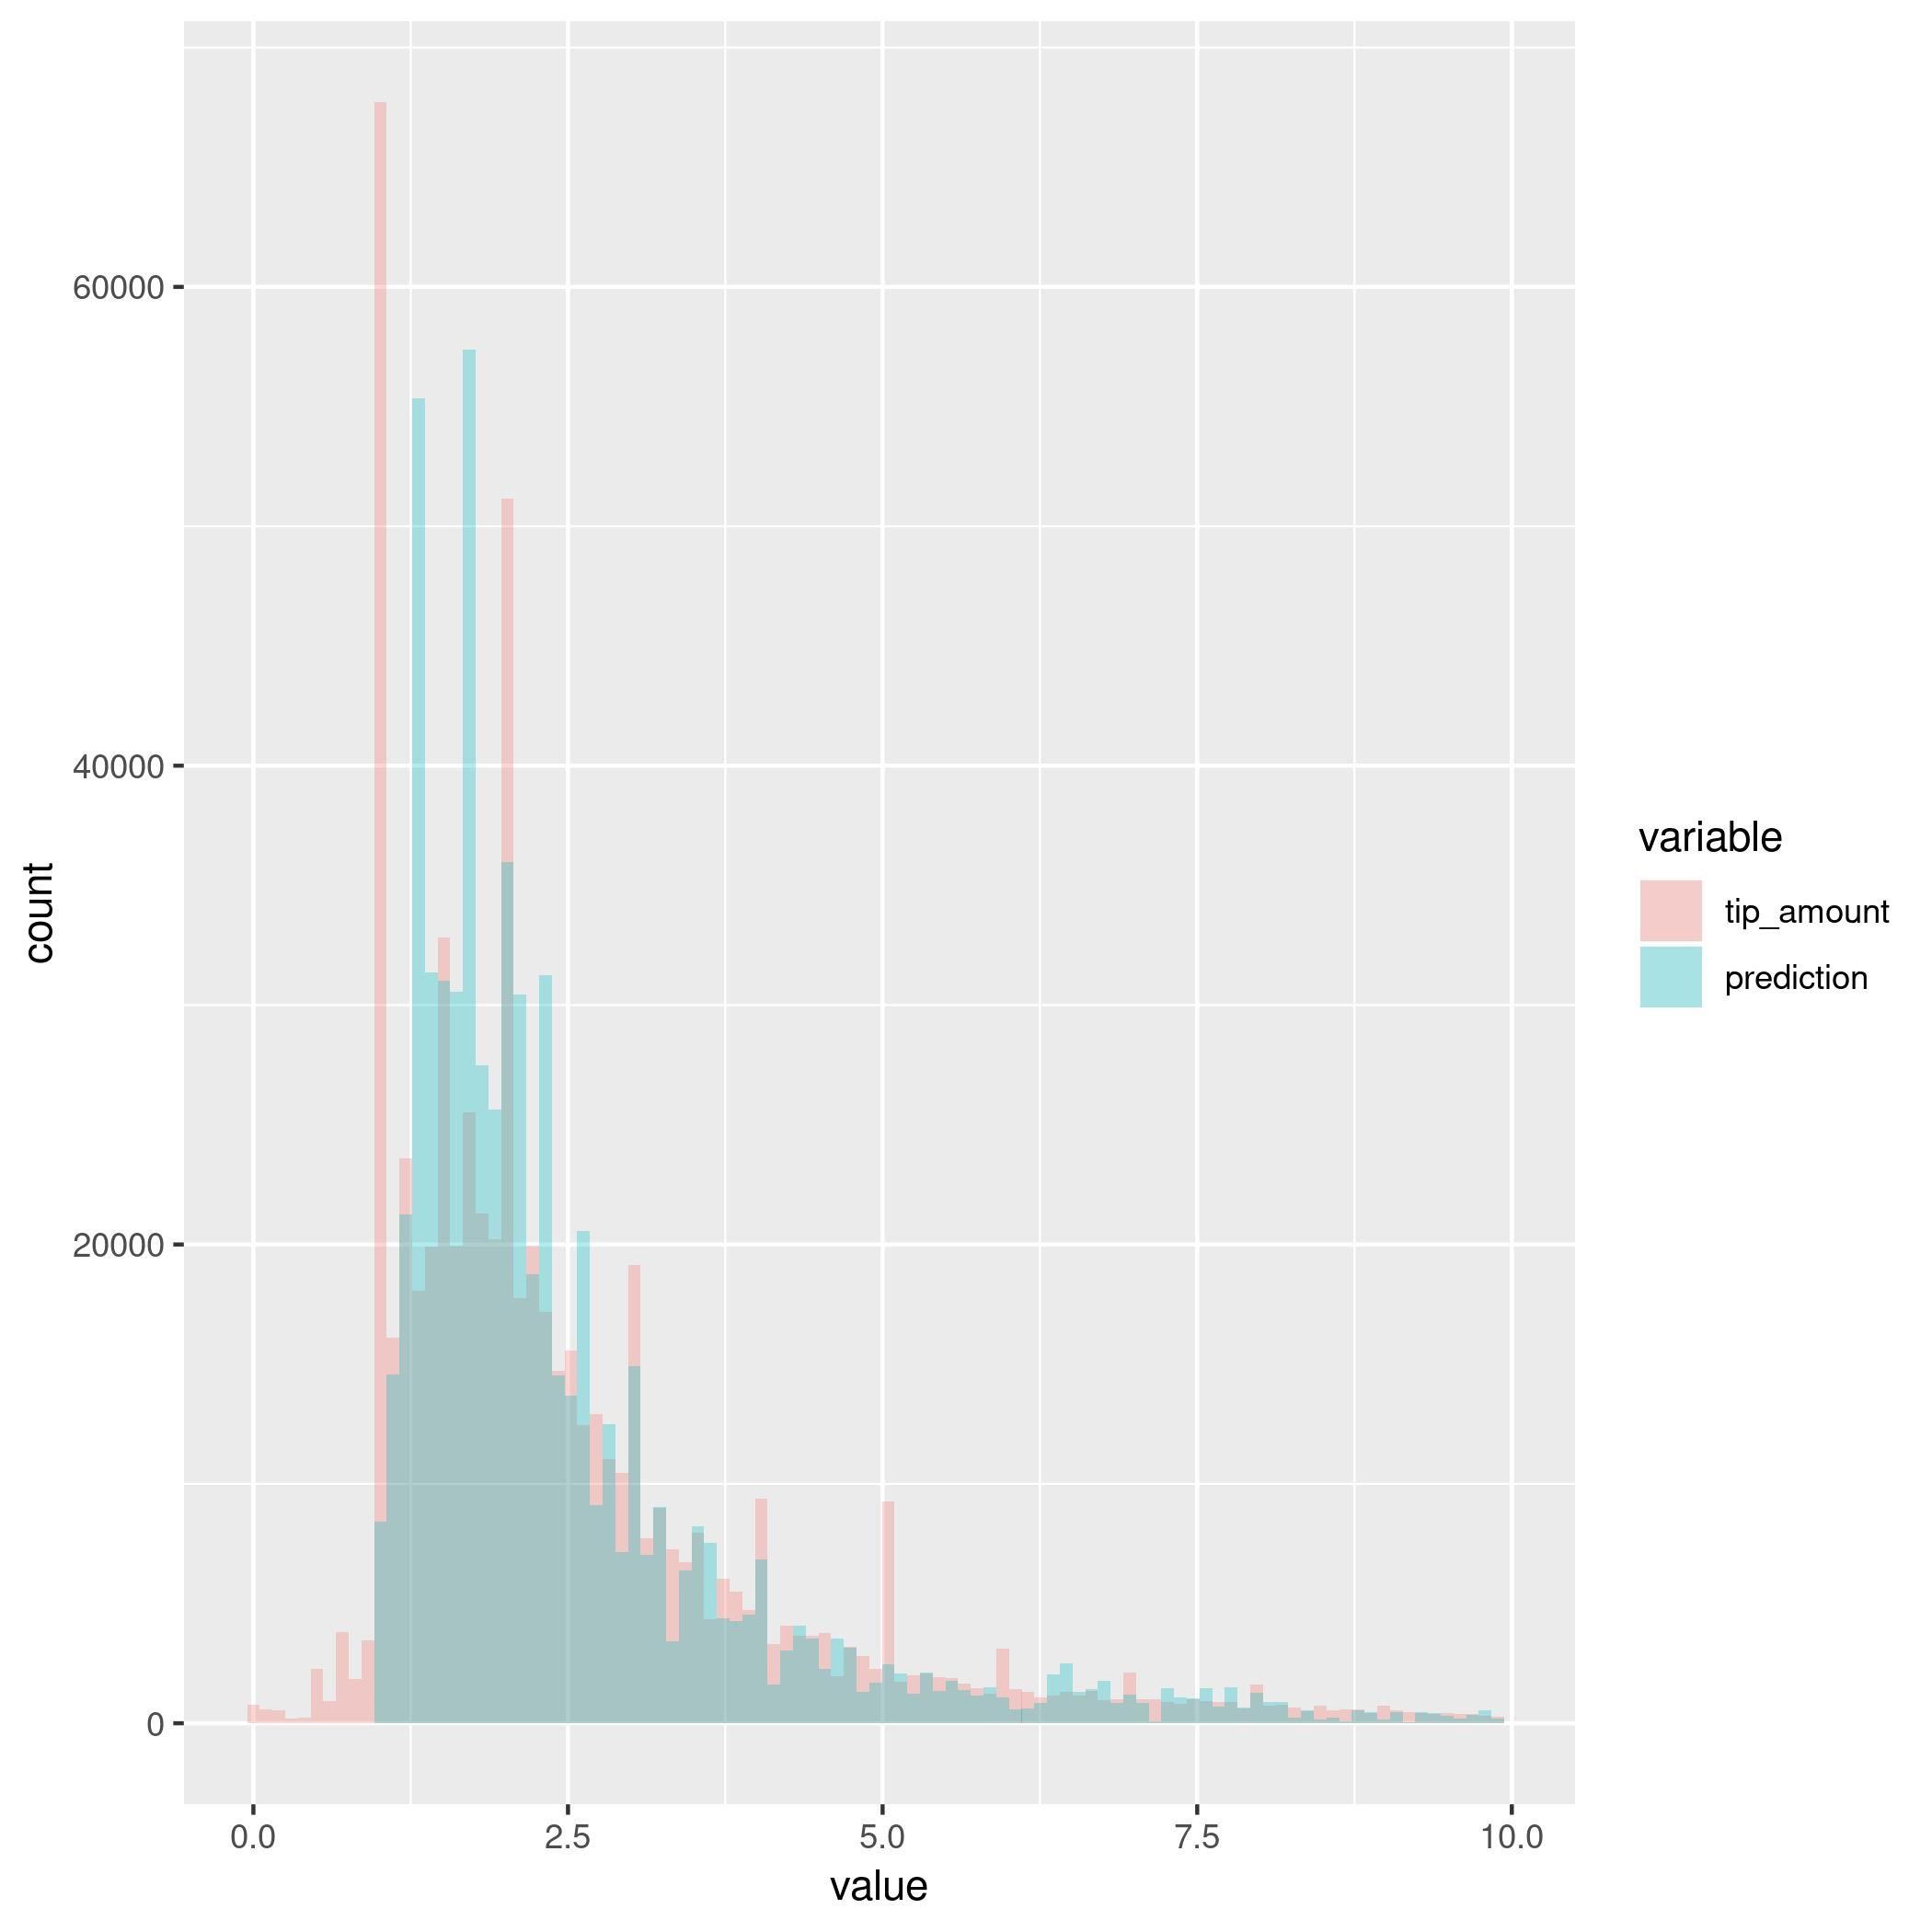
\includegraphics[width=.9\linewidth]{./plots/rfNodesize10000Maxnode100PosteriorPredictive.jpg}
\caption{\label{fig:org51b587d}
Posterior predictive evaluation with 100 nodes of size 10000}
\end{figure}

\begin{figure}[htbp]
\centering
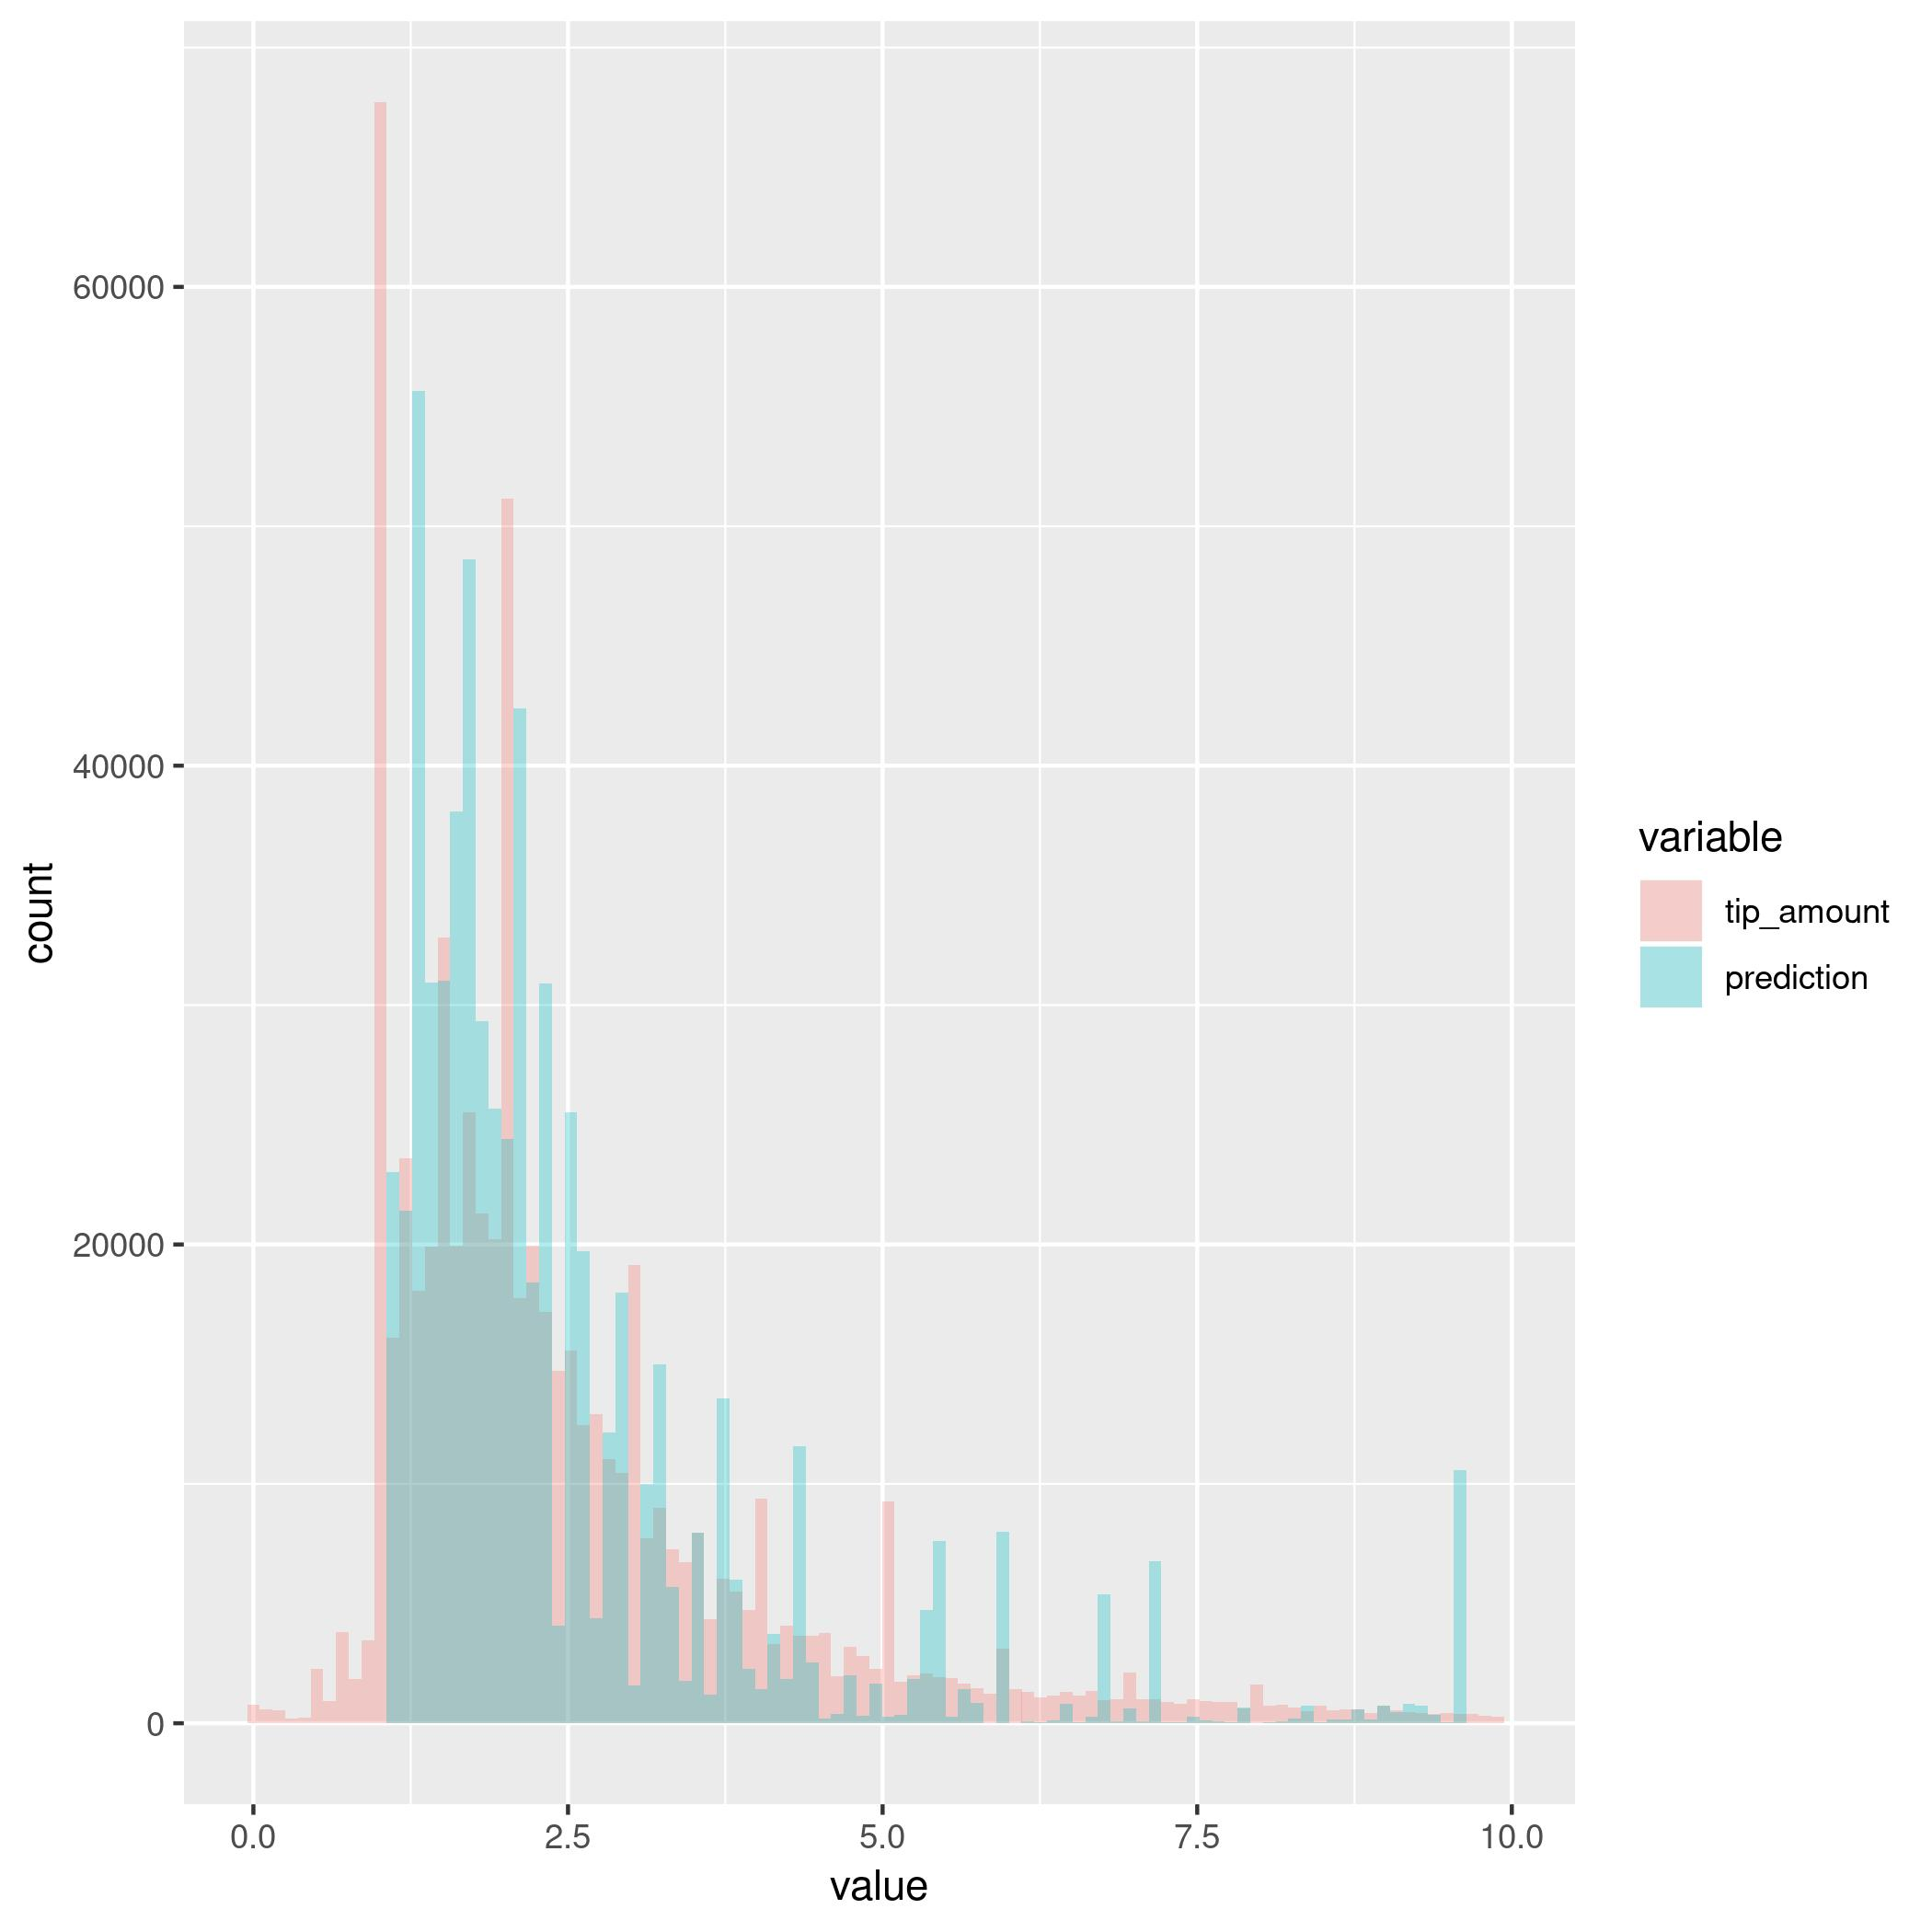
\includegraphics[width=.9\linewidth]{./plots/rfNodesize110000Maxnode30PosteriorPredictive.jpg}
\caption{\label{fig:orgad93f36}
Posterior predictive evaluation with 30 nodes of size 110000}
\end{figure}

\begin{figure}[htbp]
\centering
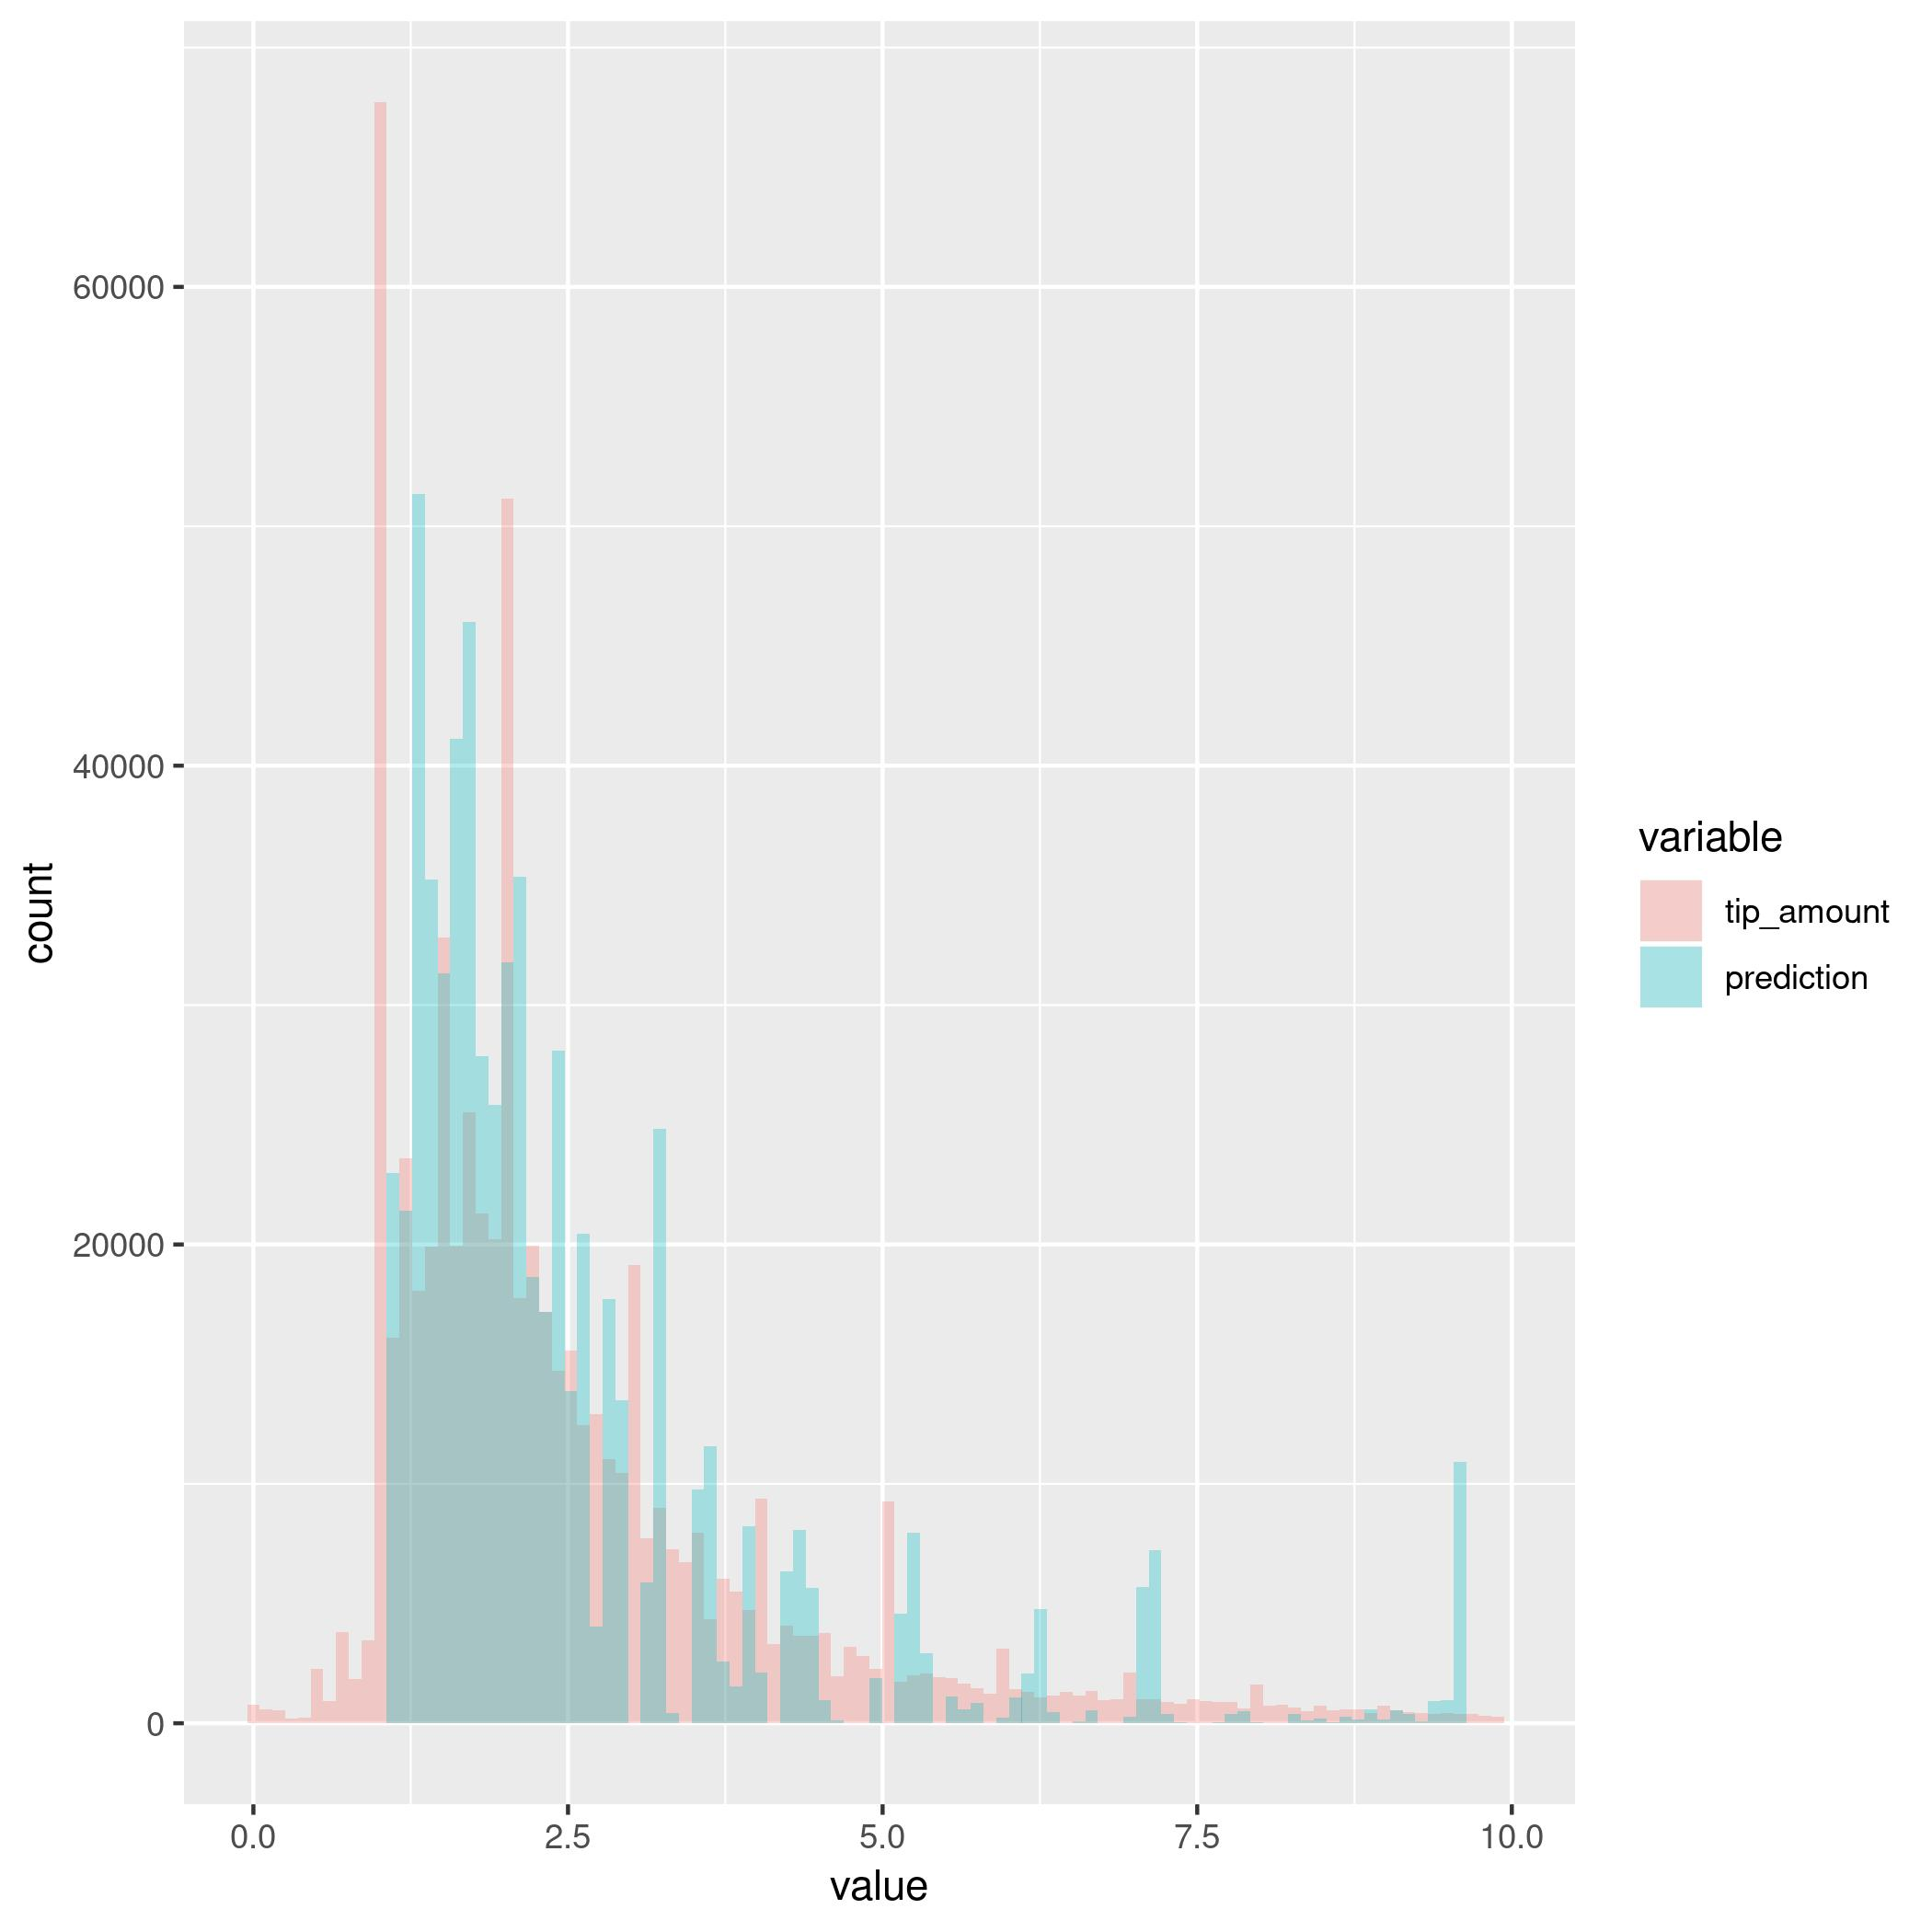
\includegraphics[width=.9\linewidth]{./plots/rfNodesize1e+05Maxnode70PosteriorPredictive.jpg}
\caption{\label{fig:org9b78f88}
Posterior predictive evaluation with 70 nodes of size 150000}
\end{figure}

\begin{figure}[htbp]
\centering
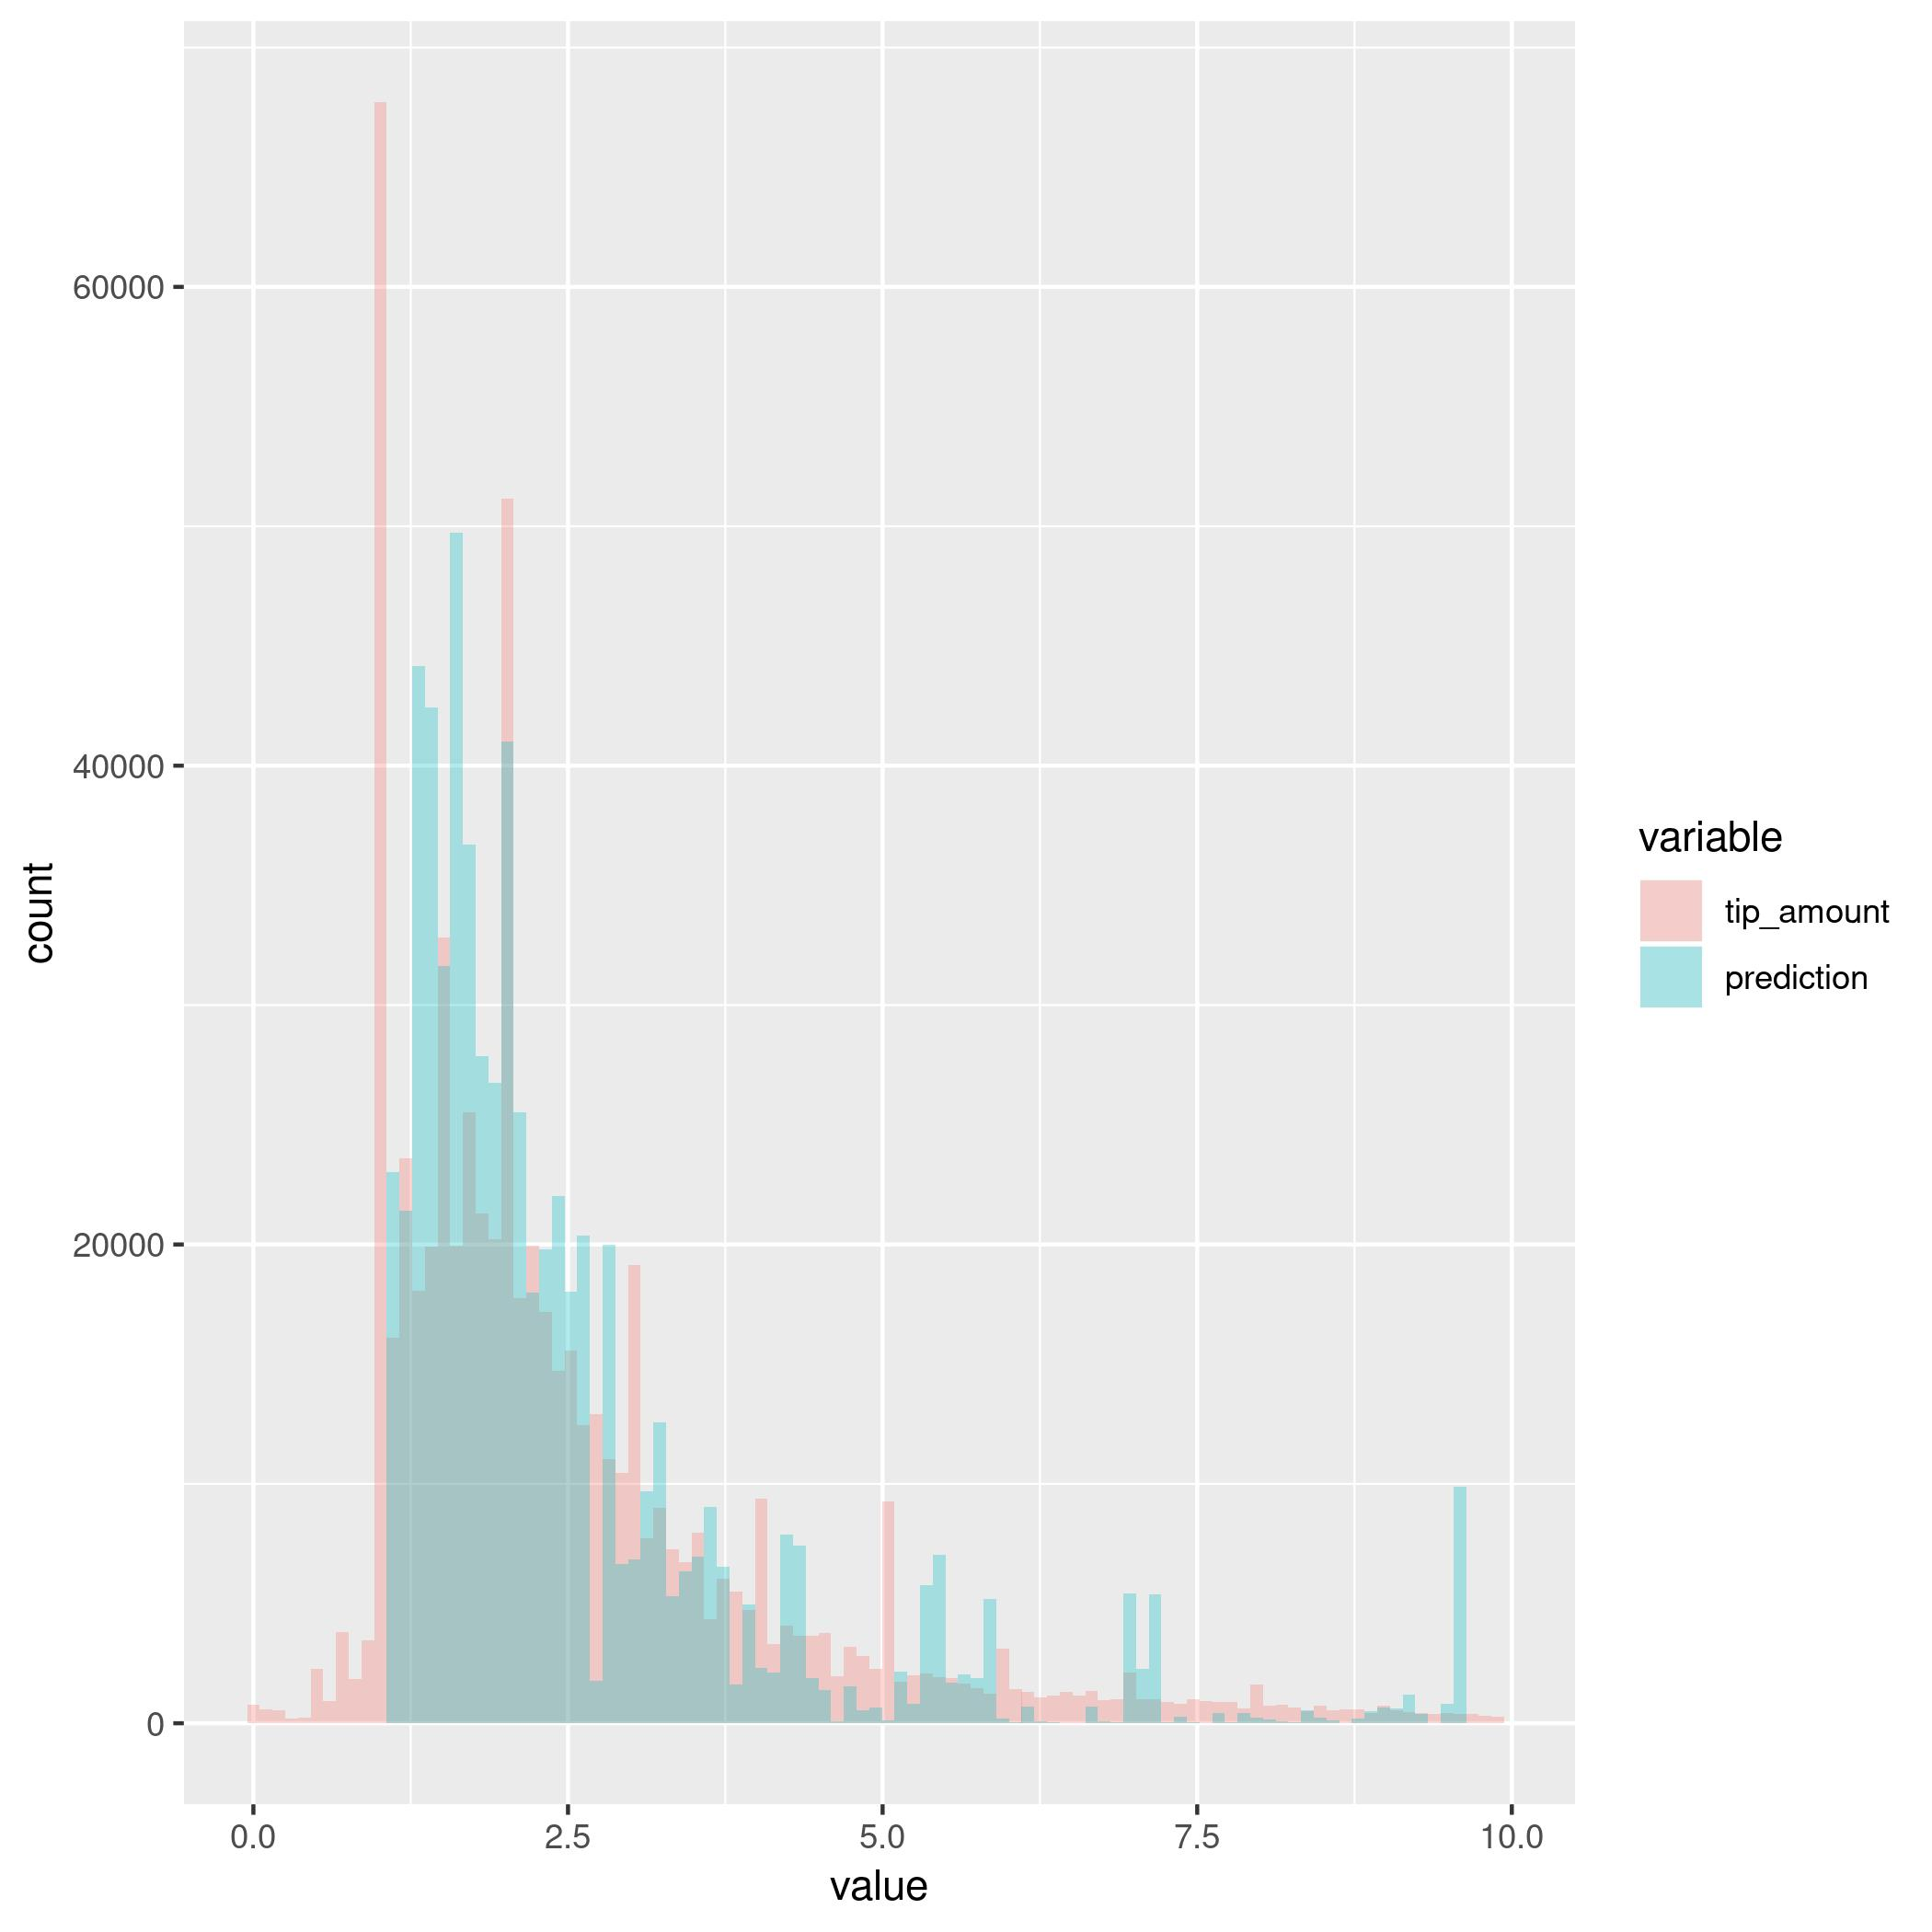
\includegraphics[width=.9\linewidth]{./plots/rfNodesize110000Maxnode50PosteriorPredictive.jpg}
\caption{\label{fig:orgdc0aa35}
Posterior predictive evaluation with 50 nodes of size 11000}
\end{figure}





\subsection{Choosing a model}
\label{sec:org5c42c4c}
Even though, the better accuracy metrics were obtained in some of the
random forest, i would choose the weighted mixed linear model.
The main reason is because the posterior predictive distribution
has a tighter fit to the data. I believe that most of the failure of the
model is due to the spike at \$1, which is hard to approximate, and as such,
i am not strongly concerned with the poor metrics.
Other nice feature of linear models is they are easy to understand, and this
makes them better thought tools to reason about our data and extend the analysis.
For example, I think an interesting next step would be to A/B test different
recommendations on the clients by their drop off destination. Another
interesting project would be to evaluate the changes of the tips provided,
given the difference between the estimated charge that is usually provided
when contracting the ride and the actual fare amount.
This would allow to figure out recomendations and figures to give the
customers in order to maximize tips for driver satisfaction. In order to
carry out these experiments, having a model that has clear effects for
all the variables is a strong feature.

The main caveat of this model, is that is linear. As such, any non linear
patterns in the data are not going to be well approximated. Furthermore,
i have been working under the assumption that the posterior predictive
distribution is a good metric for evaluation. If we were just interested
in accuracy performance, this model would be a bad choice.

Some of the things to improve in the model would be the spatial effects.
given the limited computing power I have. These effects were approximated
using borough dummies, but a better approach would be to use the full 2k
taxi zones. Furthermore, it would be interesting to implement some of the
models proposed \href{https://mc-stan.org/users/documentation/case-studies/icar\_stan.html}{here}, as from the descriptive plots it is made obvious that
the distribution of tips changes by zone.
Other interesting extension, with more months, would be to include month
dummies, in order to evaluate whether tips as higher on christmas, during
months with high tourism, etc.

Finally, it would be quite interesting to implement a mixture model,
were the tips are either distributed by a gamma (as we did in the model)
or a multinomial distribution of the values \$1, \$2, \$3, \$5. This would
nicely fit the actual data.


\subsection{How to implement as an API}
\label{sec:org942288b}
In order to implement this model as an API, I think two components would
be necessary:
\begin{itemize}
\item a service that would provide the recomendation based on the ride features
\item a backend that would update the model with the new available data
\end{itemize}

For the first component, we would need a function that, provided the
ride characteristics, would read the current state of the fitted model, and
provide the recommendation.
For the second component, whenever an update of the model is required, would
re-fit the data and serve the new model to the first component.

The most efficient way to do this would be as two concurrent processes, with
the first component activating when new models are fitted or recommendations
are required.
\end{document}
